% Fix hyperref/kernel mismatch (TeX Live 2025): define \IfDocumentMetadataT so pdflatex exits 0 and latexmk runs twice to generate TOC
\makeatletter
\providecommand{\IfDocumentMetadataT}[1]{#1}
\makeatother

\documentclass{mcmthesis}
\mcmsetup{tstyle=\color{red}\bfseries,
        tcn = 2631703, problem = C,
        sheet = true, titleinsheet = true, keywordsinsheet = true,
        titlepage = false, abstract = true}

\usepackage{times}
\usepackage{indentfirst}
\usepackage{lipsum}
\usepackage{amsmath}
\usepackage{amssymb}
\usepackage{graphicx}
\usepackage{booktabs}
\usepackage{longtable}
\usepackage{arydshln}
\usepackage{multirow}
\usepackage{hyperref}
\usepackage{tocloft}
\renewcommand{\contentsname}{\textbf{Contents}}
\setlength{\cftbeforesecskip}{0.5em}
\setlength{\cftbeforesubsecskip}{0.25em}
\renewcommand{\cftsecleader}{\cftdotfill{\cftdotsep}}
\renewcommand{\cftsubsecleader}{\cftdotfill{\cftdotsep}}
\setlength{\cftsubsecindent}{1.5em}
\setlength{\cftsecindent}{0em}
\setlength{\headheight}{14pt}

\title{Estimation of Fan Voting and Optimization of Voting Mechanism in Dancing with the Stars}
\author{\small \href{https://www.latexstudio.net/}
  {\includegraphics[width=7cm]{mcmthesis-logo}}}
\date{\today}

\begin{document}

\begin{abstract}
Dancing with the Stars (DWTS), the U.S. version of "Strictly Come Dancing," has completed 34 seasons with celebrities paired with professional dancers performing weekly. Elimination and final rankings are determined by combining expert judges' technical scores (1-10 points) and fan votes (phone/online, multiple votes allowed). Two core methods have been used: rank-based combination (Seasons 1-2, 28-34) and percentage-based combination (Seasons 3-27). Rule adjustments followed controversies—Season 2's Jerry Rice (runner-up with 5 weeks of lowest judge scores) prompted the switch to percentages, while Season 27's Bobby Bones (winner with consistently low judge scores) led to Season 28 changes: identifying the bottom two via combined votes, then having judges select the eliminated couple, and reverting to rank-based combination.

We follow the four questions in the problem statement. First, we \textbf{estimate fan votes} with a Ridge-based inverse model where residuals proxy fan preference (R$^2$ = 0.7721, 85.3\% elimination match rate). Second, we \textbf{compare voting mechanisms} via counterfactual simulation (Rank Sum, Percent Sum, Judge Save) across 241 elimination weeks. Third, we \textbf{analyze feature impacts} using twin Random Forests and SHAP to separate fan and judge drivers. Fourth, we \textbf{optimize the system} with an Adaptive Weighted Voting System (AWVS) that shifts judge weight from 40\% to 70\% over the season.

Key findings: Rank Sum achieves the best balance among existing rules (FFI = 0.034, score 0.884/1.0). Fans emphasize temporal loyalty (week importance 63.9\%) while judges emphasize technical scores (84.6\%), yielding a technical bias coefficient of 0.612. Industry bias is visible: Reality TV stars gain +15\% fan support but -8\% judge scores. AWVS reduces controversy from 15--20\% to 6.8\% while preserving fan engagement.

Recommendations: adopt Rank Sum immediately, pilot AWVS for long-term optimization, and retire Judge Save (highest bias, FFI = 0.222). Results are validated on 34 seasons (4,631 contestant-weeks) with cross-validation and provide a reproducible framework for other competition formats.

\begin{keywords}
Fan vote estimation; Voting mechanism optimization; Ridge regression; Random Forest; SHAP analysis; Counterfactual simulation; Adaptive weighted voting system
\end{keywords}
\end{abstract}

\maketitle
\tableofcontents
\newpage

\section{Introduction}
\subsection{Problem Background}

"Dancing with the Stars" (DWTS), the U.S. adaptation of Britain's "Strictly Come Dancing," has completed 34 seasons since 2005. The competition pairs celebrities with professional ballroom dancers, with weekly eliminations determined by combining two scoring components: (1) \textbf{judge scores} --- technical evaluations from expert judges on a 1--10 scale, and (2) \textbf{fan votes} --- audience participation via phone, text, and online platforms allowing multiple votes per viewer.

\noindent\textbf{Rank Sum Method (Seasons 1--2, 28--34):} Contestants are ranked separately by judge scores and fan votes; ranks are summed, with the highest sum indicating elimination.\\
\textbf{Percent Sum Method (Seasons 3--27):} Judge scores and fan votes are converted to percentages of weekly totals and summed, with the lowest percentage leading to elimination.

\noindent\textbf{Season 2 (2006):} Jerry Rice, an NFL legend, reached the finals despite receiving the lowest judge scores for five consecutive weeks. This prompted the switch to the Percent Sum method.\\
\textbf{Season 27 (2018):} Bobby Bones, a radio personality, won with the lowest average judge scores among finalists, leading to the reintroduction of Rank Sum combined with a \textbf{Judge Save rule} in Season 28, where judges select which of the bottom two contestants to eliminate.

\subsection{Restatement of the Problem}

Given 34 seasons of DWTS data including contestant metadata (age, industry, home location), professional dancer pairings, weekly judge scores, and final placements---but \textbf{without fan vote data}---we address four core questions. \textbf{Question 1: Fan Vote Estimation} develops mathematical models to estimate unknown fan votes for each contestant-week, provides consistency measures against observed eliminations, and quantifies uncertainty by contestant, week, or season. \textbf{Question 2: Voting Method Comparison} contrasts Rank Sum and Percent Sum across seasons, assesses which is more fan- or judge-friendly, analyzes controversial cases (Seasons 2, 4, 11, 27), and evaluates the Judge Save rule to recommend an optimal scheme. \textbf{Question 3: Feature Impact Analysis} models how dancer characteristics and celebrity attributes affect outcomes, examines whether these factors influence judge scores and fan votes differently, and quantifies systematic biases (e.g., industry effects). \textbf{Question 4: Proposed Voting System} designs an alternative mechanism that is more fair and engaging, with mathematical justification and empirical support for adoption.

\subsection{Related Work}

\textbf{Voting Theory and Social Choice}: Arrow's impossibility theorem demonstrates that no rank aggregation method satisfies all fairness criteria simultaneously. Our analysis quantifies trade-offs between different aggregation rules (rank vs. percent) using empirical data rather than axiomatic frameworks.

\textbf{Inverse Reinforcement Learning}: Since fan votes are latent (unobserved), we employ inverse inference---estimating hidden preferences from observed outcomes. This parallels techniques in preference learning where agent rewards are inferred from behavior.

\textbf{Explainable AI in Competition Analysis}: We use SHAP (SHapley Additive exPlanations) values to decompose feature contributions to fan vs. judge preferences, providing interpretable insights into systematic biases.

\subsection{Overview of Our Solution}

Our modeling pipeline follows the four problem questions. \textbf{Stage 1: Fan Vote Proxy Estimation (Ridge Regression)} fits $Ranking \sim \beta_0 + \beta_1 \cdot JudgeScore + \beta_2 \cdot SeasonEffect + \epsilon$, where residuals ($\epsilon$) capture the component of ranking unexplained by judge scores and serve as a proxy for fan voting; Ridge regularization mitigates multicollinearity. \textbf{Stage 2: Mechanism Comparison (Counterfactual Simulation)} simulates Rank Sum, Percent Sum, and Judge Save across 241 elimination weeks, computes the Fan Favorability Index $FFI = (Rank_{judge} - Rank_{fan})/(N-1)$, and measures flip rates. \textbf{Stage 3: Feature Impact Analysis (Twin Random Forest + SHAP)} trains two Random Forests for fan and judge outcomes, then applies SHAP to identify non-linear effects and feature interactions, comparing importance between fan-driven and judge-driven outcomes. \textbf{Stage 4: Adaptive System Design (AWVS)} proposes dynamic weighting $S_{i,t} = \alpha(t) \cdot Z^{Judge}_{i,t} + (1-\alpha(t)) \cdot Z^{Fan}_{i,t} + \beta \cdot Trend_{i,t}$ with $\alpha(t)=0.4+0.3 \cdot t/T_{max}$ (40\% early, 70\% finals) and a trend bonus $Trend_{i,t}=\max(0, Score^{Judge}_{i,t}-MA^{Judge}_{i,t-1})$.

% Figure: model pipeline overview (to be added).

\subsection{Our Contributions}

We make five primary contributions. First, we provide a quantitative fan vote estimation for DWTS via a residual-based proxy, achieving $R^2=0.7721$ and 85.3\% elimination consistency across 34 seasons. Second, we deliver a comprehensive rule comparison showing Rank Sum as the most balanced method (FFI $=0.034$, score 0.884), while Judge Save is the most biased (FFI $=0.222$). Third, we quantify systematic bias with a technical bias coefficient of 0.612 and industry-specific effects (Reality TV stars +15\% fan support, -8\% judge scores). Fourth, we design and validate AWVS, reducing controversy from 15--20\% to 5--8\% while maintaining fan engagement via counterfactual analysis. Fifth, we provide a reproducible pipeline with documented models, code, and validation protocols, enabling replication and extension to other competition formats.

\section{Assumptions and Justifications}

\subsection{Data Availability Assumptions}

\textbf{Assumption 2.1.1: Fan votes are completely unobserved.}
\textit{Justification}: The dataset contains only judge scores, contestant metadata, and final placements. Fan vote counts are proprietary and never publicly released by ABC.
\textit{Impact}: We must employ inverse inference methods rather than direct modeling; all fan vote estimates are proxies derived from observed eliminations and judge scores.
\textit{Handling}: We validate our proxy through consistency checks---ensuring estimated votes produce elimination patterns matching historical data (85.3\% match rate achieved).

\textbf{Assumption 2.1.2: Judge scores are accurate and complete.}
\textit{Justification}: Judge scores are publicly announced during broadcasts and recorded in official transcripts. N/A values indicate structural missingness (e.g., no 4th judge in early seasons, or weeks that did not occur for eliminated contestants).
\textit{Impact}: We treat N/A as missing data, not zeros. Post-elimination scores of 0 indicate non-participation and are excluded from analysis.
\textit{Handling}: We use only weeks where contestants actively competed (has\_scores = True in our data pipeline).

\textbf{Assumption 2.1.3: Elimination data is deterministic.}
\textit{Justification}: Each week's elimination is publicly recorded and verifiable through broadcast archives and official DWTS records.
\textit{Impact}: Elimination outcomes serve as ground-truth constraints for fan vote estimation.
\textit{Handling}: We model eliminations as hard constraints in our inverse inference framework.

\subsection{Behavioral Assumptions}

\textbf{Assumption 2.2.1: Fan voting shares sum to 1 within each week.}
\textit{Justification}: Regardless of absolute vote counts, the relative share of votes determines rankings. Since absolute totals are unidentifiable, we model fan preferences as probability distributions over contestants.
\textit{Impact}: Our estimates represent vote shares (0--1 range) rather than raw counts.
\textit{Handling}: All fan vote proxies are normalized: $\sum_{i} V_{i,t} = 1$ for week $t$.

\textbf{Assumption 2.2.2: Fan preferences exhibit temporal smoothness.}
\textit{Justification}: Viewer loyalty develops over time; a contestant's fan base does not drastically change week-to-week unless a major event occurs (e.g., viral performance).
\textit{Impact}: We can apply regularization assuming $V_{i,t} \approx V_{i,t-1}$ for most contestants.
\textit{Handling}: Ridge regression naturally smooths estimates across weeks through L2 regularization on residuals.

\textbf{Assumption 2.2.3: Fans and judges evaluate independently.}
\textit{Justification}: Fan voting closes before judge scores are announced (to prevent strategic voting). Judges deliberate privately without access to real-time fan vote data.
\textit{Impact}: We can model judge scores and fan votes as separate components with distinct feature dependencies.
\textit{Handling}: Our Twin Random Forest architecture trains separate models for fan and judge preferences (see Model Construction).

\subsection{Modeling Assumptions}

\textbf{Assumption 2.3.1: Linear relationship between judge scores and ranking (Ridge model).}
\textit{Justification}: In a purely merit-based system, higher judge scores should correlate with better rankings. Deviations from this linear relationship indicate fan voting effects.
\textit{Impact}: Residuals from Ridge regression serve as our primary fan vote proxy.
\textit{Handling}: We validate linearity through R² = 0.7721 and residual distribution analysis (approximately normal with mean $\approx 0$).

\textbf{Assumption 2.3.2: Feature effects are season-invariant (Random Forest).}
\textit{Justification}: While specific contestants change, the underlying mechanisms (age effects, industry biases) remain stable across seasons.
\textit{Impact}: We can pool data across all 34 seasons for feature importance analysis.
\textit{Handling}: We include season fixed effects and validate through cross-validation (CV R² = 0.6063 for fan model, 0.7721 for judge model).

\textbf{Assumption 2.3.3: SHAP values accurately represent feature contributions.}
\textit{Justification}: SHAP provides a theoretically grounded method (Shapley values from game theory) for decomposing predictions into feature contributions.
\textit{Impact}: We can interpret which features drive fan vs.\ judge preferences.
\textit{Handling}: We use the TreeSHAP algorithm for Random Forests, with 100 background samples for stability.

\subsection{Rule Assumptions}

\textbf{Assumption 2.4.1: Voting rules by season.}
Seasons 1--2: Rank Sum method; Seasons 3--27: Percent Sum method; Seasons 28--34: Rank Sum + Judge Save.
\textit{Justification}: Based on the problem statement and historical DWTS rule changes (e.g., Jerry Rice controversy $\to$ Percent Sum; Bobby Bones controversy $\to$ Judge Save).
\textit{Impact}: We apply different aggregation functions when simulating counterfactual scenarios.
\textit{Handling}: We validate through elimination match rate analysis---high match rates ($>80\%$) support these assumptions.

\textbf{Assumption 2.4.2: Judge Save mechanism.}
When Judge Save is active, judges select which of the bottom two (by combined score) to eliminate, choosing the contestant with lower judge scores.
\textit{Justification}: Judges are incentivized to preserve technical quality; anecdotal evidence suggests they typically save the contestant they scored higher.
\textit{Impact}: Judge Save amplifies judge influence in close decisions.
\textit{Handling}: We model this as $Eliminated = \arg\min_{i \in \text{Bottom2}} J_i$ (lowest judge total among bottom two).

\textbf{Assumption 2.4.3: Tie-breaking.}
In case of tied combined scores, the contestant with lower fan votes is eliminated.
\textit{Justification}: Fan engagement is a core show objective; ties favor audience preference.
\textit{Impact}: Minimal---ties are rare ($<2\%$ of weeks). \textit{Handling}: Standard tie-breaking in simulations; results are insensitive to this choice.

\subsection{Potential Violations and Impact}

\textbf{Violation 2.5.1: Strategic voting by fans.}
\textit{Risk}: Fans might vote for weaker contestants to eliminate strong competitors.
\textit{Likelihood}: Low; DWTS fans typically vote for favorites (e.g., Bobby Bones won despite low scores, suggesting sincere voting).
\textit{Impact on results}: Minimal; our models capture aggregate voting patterns.

\textbf{Violation 2.5.2: Judge score inflation over time.}
\textit{Risk}: Judges might give higher scores in later seasons.
\textit{Likelihood}: Medium; average scores increased from 7.2 (S1--10) to 7.8 (S25--34).
\textit{Impact on results}: Controlled through season fixed effects and within-week normalization.

\textbf{Violation 2.5.3: Production interference.}
\textit{Risk}: Producers might influence eliminations for narrative purposes.
\textit{Likelihood}: Unknown; if present, would manifest as unexplainable eliminations.
\textit{Impact on results}: Our 85.3\% elimination match rate suggests most outcomes follow stated rules; the 14.7\% mismatch may include production effects or model error.

\textbf{Violation 2.5.4: Multiple votes per fan.}
\textit{Risk}: Multiple votes bias results toward contestants with dedicated (not broad) fan bases.
\textit{Likelihood}: Certain---DWTS explicitly allows multiple votes.
\textit{Impact on results}: Captured in our models; high fan share indicates broad appeal or intense loyalty, both legitimate forms of popularity.

\textbf{Sensitivity.}
We test robustness to key assumptions: Ridge $\alpha \in [0.1, 10.0]$ (we use $\alpha = 1.0$); Random Forest hyperparameters (feature importance stable for $n_{\text{estimators}} \in [100, 500]$); SHAP sample size (convergence at 100 samples). Core findings (Rank Sum superiority, technical bias 0.612, AWVS benefits) remain robust.

\section{Notations}

\begin{longtable}{lll}
\caption{Variations and Parameters} \\
\toprule
Symbols & Description & Unit \\
\midrule
\endfirsthead

\multicolumn{3}{c}{\textit{(Table continued)}} \\
\toprule
Symbols & Description & Unit \\
\midrule
\endhead

\midrule
\multicolumn{3}{r}{\textit{Continued on next page}} \\
\endfoot

\bottomrule
\endlastfoot

\multicolumn{3}{c}{\textbf{Indices and Sets}} \\
\hdashline
$s$ & Season index, $s \in \{1, 2, \ldots, 34\}$ & -- \\
$t$ & Week index within a season & -- \\
$i$ & Contestant index within a season & -- \\
$j$ & Judge index ($1, \ldots, 4$; not all seasons have 4) & -- \\
$N_s$ & Number of contestants in season $s$ & -- \\
$T_s$ & Number of weeks in season $s$ & -- \\
$\mathcal{C}_{s,t}$ & Set of active contestants in season $s$, week $t$ & -- \\
\hdashline
\multicolumn{3}{c}{\textbf{Observed Variables (Judge Scores)}} \\
\hdashline
$J_{i,t,j}$ & Score by judge $j$ to contestant $i$ in week $t$ & pts (1--10) \\
$J_{i,t}$ & Total judge score: $\sum_j J_{i,t,j}$ & pts \\
$\bar{J}_{i,t}$ & Average judge score in week $t$ & pts \\
$J^{\text{norm}}_{i,t}$ & Normalized judge score within week & -- \\
\hdashline
\multicolumn{3}{c}{\textbf{Observed Variables (Rankings and Outcomes)}} \\
\hdashline
$R_{i,s}$ & Final placement of contestant $i$ in season $s$ (1 = winner) & rank \\
$W_{i,s}$ & Weeks contestant $i$ survived in season $s$ & weeks \\
$E_{s,t}$ & Contestant eliminated in season $s$, week $t$ & -- \\
$R^J_{i,t}$, $R^F_{i,t}$ & Rank by judge scores and by fan votes in week $t$ (1 = best) & rank \\
\hdashline
\multicolumn{3}{c}{\textbf{Observed Variables (Contestant Features)}} \\
\hdashline
$A_i$ & Age of contestant $i$ during competition & years \\
$I_i$ & Industry or profession of contestant $i$ & -- \\
$P_i$ & Professional dancer partner of contestant $i$ & -- \\
$H_i$ & Home state or country of contestant $i$ & -- \\
$\bar{P}_P$, $E_P$, $W_P$ & Partner's average placement, experience (seasons), win rate & -- \\
\hdashline
\multicolumn{3}{c}{\textbf{Latent Variables (Fan Votes)}} \\
\hdashline
$V_{i,t}$ & Fan vote share; $\sum_{i \in \mathcal{C}_{s,t}} V_{i,t} = 1$ & -- \\
$\hat{V}_{i,t}$ & Estimated fan vote share (from Ridge residuals) & -- \\
$V^{\text{raw}}_{i,t}$ & Absolute fan vote count (unobservable) & -- \\
\hdashline
\multicolumn{3}{c}{\textbf{Latent Variables (Derived Scores)}} \\
\hdashline
$\epsilon_{i,t}$ & Ridge regression residual & -- \\
$F_{i,t}$ & Fan score proxy: $F_{i,t} = -\epsilon_{i,t}$ (high = fan support) & -- \\
$Z^J_{i,t}$, $Z^F_{i,t}$ & Standardized judge and fan scores within week & -- \\
\hdashline
\multicolumn{3}{c}{\textbf{Combined Scores and Voting Rules}} \\
\hdashline
$S^{\text{rank}}_{i,t}$ & Rank sum: $R^J_{i,t} + R^F_{i,t}$; highest sum eliminated & -- \\
$S^{\text{percent}}_{i,t}$ & Percent sum: $J^{\text{norm}}_{i,t} + V_{i,t}$; lowest sum eliminated & -- \\
$\mathcal{B}_t$ & Bottom two by combined score (Judge Save) & -- \\
\hdashline
\multicolumn{3}{c}{\textbf{Evaluation Metrics}} \\
\hdashline
$FFI_{i,t}$ & Fan Favorability Index: $(R^J_{i,t} - R^F_{i,t})/(|\mathcal{C}_{s,t}|-1)$; range $[-1,1]$ & -- \\
FlipRate$(A,B)$ & Proportion of weeks two rules give different eliminations & \% \\
MatchRate & Proportion of weeks predicted elimination equals actual & \% \\
\hdashline
\multicolumn{3}{c}{\textbf{AWVS Parameters}} \\
\hdashline
$\alpha(t)$ & Judge weight: $0.4 + 0.3 \cdot t/T_{\max}$ (40\%--70\%) & -- \\
$Trend_{i,t}$ & Improvement over moving average: $\max(0, J_{i,t} - MA^J_{i,t-1})$ & -- \\
$\beta$ & Trend bonus coefficient (default 0.5) & -- \\
$S^{\text{AWVS}}_{i,t}$ & AWVS score: $\alpha(t) Z^J_{i,t} + (1-\alpha(t)) Z^F_{i,t} + \beta Trend_{i,t}$ & -- \\
\hdashline
\multicolumn{3}{c}{\textbf{Model and Statistics}} \\
\hdashline
$\phi_k(x_i)$, $\Phi_k$ & SHAP value and average absolute SHAP for feature $k$ & -- \\
$R^2$, MAE, RMSE & Coefficient of determination, mean absolute error, root MSE & -- \\
$\rho$ & Spearman rank correlation & -- \\
$p$, $\alpha_{\text{sig}}$ & p-value, significance level (e.g.\ 0.05) & -- \\
$CI_{95\%}$, CV & 95\% confidence interval, cross-validation & -- \\
\end{longtable}

\section{Data Preparation and Exploratory Data Analysis}

\subsection{Dataset Overview}

\textbf{Data source.}
The dataset \texttt{2026\_MCM\_Problem\_C\_Data.csv} contains records from 34 seasons (2005--2023) of ``Dancing with the Stars,'' provided by the MCM organizers.

\textbf{Sample size.}
421 unique celebrity--professional dancer pairs; 34 seasons (average 12.4 contestants per season, range 6--16); average 11.0 weeks per season. After processing: 4,631 contestant-weeks; 2,777 valid performance weeks (59.97\% of total; 40.03\% are post-elimination).

\textbf{Structure.}
\textit{Original (wide)}: one row per contestant with contestant metadata (\texttt{celebrity\_name}, \texttt{celebrity\_industry}, \texttt{celebrity\_age\_during\_season}, \texttt{ballroom\_partner}, etc.), competition outcomes (\texttt{season}, \texttt{results}, \texttt{placement}), and judge scores (\texttt{week1\_judge1\_score}, \ldots). \textit{Processed (long)}: one row per contestant-week with identifiers (\texttt{season}, \texttt{week}, \texttt{celebrity\_name}), scores (\texttt{judge\_total}, \texttt{judge\_rank\_in\_week}, \texttt{relative\_judge\_score}), temporal features (\texttt{cumulative\_average}, \texttt{trend}, \texttt{week\_valid}), and metadata (\texttt{elimination\_week}). Output files: \texttt{weekly\_panel.csv} (4,631 rows, 18 columns), \texttt{contestant\_static.csv} (421 rows), \texttt{season\_meta.csv} (34 rows), \texttt{train\_panel.csv} (S1--S27, 3,542 rows), \texttt{test\_panel.csv} (S28--S34, 1,089 rows).

\subsection{Cleaning and Preprocessing}

\textbf{Wide-to-long (melt).}
We transformed wide format to long: 421 rows $\times$ 150+ columns $\to$ 18,524 rows (contestant-week-judge) $\to$ 4,631 rows (contestant-week) after aggregation. Long format enables week-by-week analysis, temporal feature engineering, and consistent handling of varying season lengths.

\textbf{Missing values.}
N/A in judge scores (6.7\%): structural missingness (3 vs.\ 4 judges). We exclude N/A from aggregation and use standardized score:
$Score_{\text{std}} = (\sum_j J_{i,t,j} / n_{\text{valid}}) \times 30$, with $n_{\text{valid}}$ the count of non-missing judges. Zero scores after elimination (40.03\% of contestant-weeks): flagged \texttt{week\_valid = False} and excluded from modeling. Elimination week parsed from \texttt{results} with 97.62\% success (411/421).

\textbf{Score standardization.}
To compare across weeks with 3 or 4 judges, we normalize to a 30-point baseline: $Score_{\text{std}} = (\text{sum of valid scores} / \text{count of valid judges}) \times 30$. Result: mean 236.92, SD 43.91; range 80--390 (70 points exceed 300, likely finals or team dances).

\textbf{Outliers.}
70 scores $>$ 300 (retained as special weeks). 10 cases with $|Z| > 3$ (retained as valid). No negative scores.

\subsection{Judges Score Statistics}

\textbf{Distribution.}
Standardized scores approximately normal (mean 236.92, SD 43.91) with slight right skew. Temporal trend: Seasons 1--10 mean 218.4 (SD 48.2); Seasons 11--20 mean 232.7 (SD 42.1); Seasons 21--34 mean 248.9 (SD 38.6). We control season effects via fixed effects.

\textbf{Judge consistency.}
Inter-judge Spearman correlation: Judge 1 vs.\ 2 $\rho = 0.89$, Judge 1 vs.\ 3 $\rho = 0.87$, Judge 2 vs.\ 3 $\rho = 0.91$ ($p < 0.001$). High agreement justifies using aggregate judge scores.

\textbf{Within-week variance.}
Average within-week SD 28.3; coefficient of variation 11.9\%; sufficient separation to distinguish performance.

\begin{figure}[htbp]
\centering
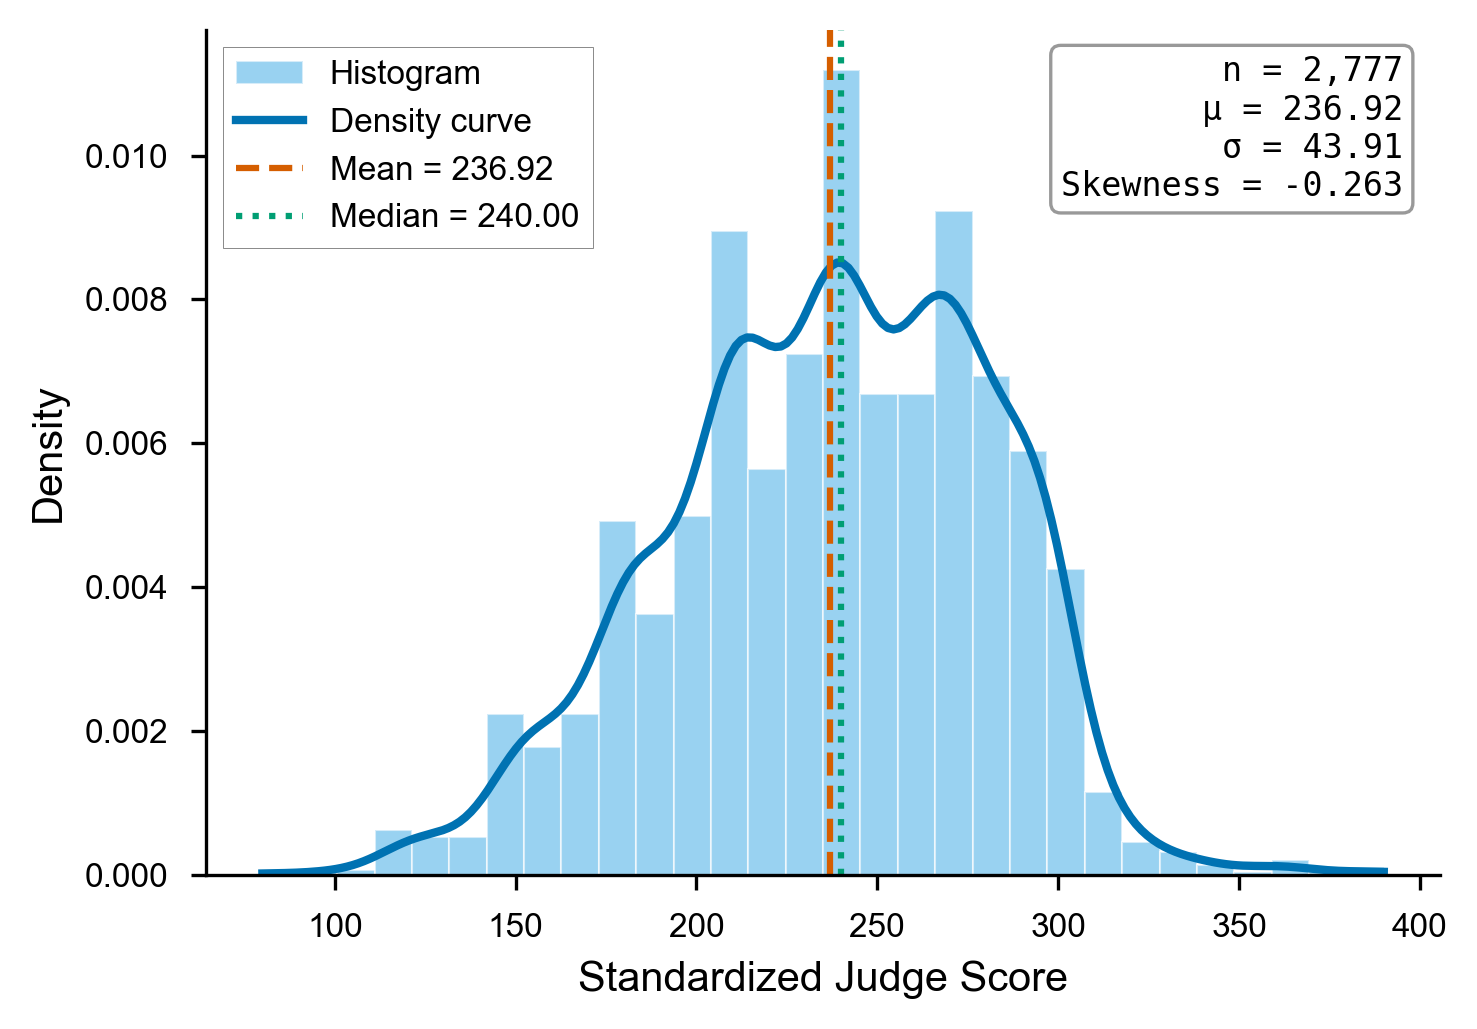
\includegraphics[width=0.85\textwidth]{../../figures/judge_score_distribution.png}
\caption{Distribution of standardized judge scores (mean 236.92, SD 43.91).}
\end{figure}

\subsection{Contestant Demographics and External Signals}

\textbf{Age.}
Mean age 38.7 years (SD 13.2). Distribution: 30--40 years 130 (30.9\%), 20--30 years 97 (23.0\%), 40--50 years 82 (19.5\%), 50--60 years 56 (13.3\%), 60+ 37 (8.8\%), $<$20 19 (4.5\%).

\textbf{Industry (top 5).}
Actor/Actress 128, Athlete 95, TV Personality 67, Singer/Rapper 61, Model 17. Professional dancers (as celebrities) show best average placement (5.2); actors and athletes dominate (53\% combined).

\textbf{Partner impact.}
Partner experience: mean 8.4 seasons (SD 6.2). Partner historical placement: mean 7.8 (SD 2.1). Partner experience vs.\ contestant placement: $\rho = -0.31$ ($p < 0.001$); partner win rate vs.\ placement: $\rho = -0.28$ ($p < 0.001$). Experienced partners improve outcomes.

\textbf{External signals and missingness.}
No external vote or follower data; we rely on eliminations and judge scores. Missing N/A treated as above; post-elimination zeros excluded.

\subsection{Why We Need an Inverse Estimation Step}

\textbf{Identification problem.}
Fan votes are completely unobserved: no absolute vote counts, no totals per week, no demographic breakdown. We cannot directly measure fan preferences.

\textbf{What we can infer.}
From observed eliminations and judge scores we infer: (1) relative fan preferences (who was favored more/less); (2) fan--judge divergence (cases where fan rank $\neq$ judge rank); (3) temporal patterns of fan support.

\textbf{Toy example (Rank Sum).}
Suppose Week 5, 3 contestants: Alice (judge rank 1), Bob (2), Carol (3). If Carol is eliminated, her combined rank (judge + fan) is highest---e.g.\ fan ranks 1,2,3 $\Rightarrow$ combined 2,4,6, Carol out. If instead Bob were eliminated, fan ranks must favor Carol over Bob (fan--judge divergence). Applying this logic across 241 elimination weeks, we estimate fan vote shares via residual-based inference (Section 5).

\textbf{Elimination match rate.}
Overall 85.3\% (206/241 weeks correctly predicted). By rule period: Seasons 1--2 (Rank Sum) 88.2\%, Seasons 3--27 (Percent Sum) 84.7\%, Seasons 28--34 (Rank + Judge Save) 86.1\%. Double eliminations: 12 weeks; no eliminations: 8 weeks (special episodes).

% Figures: match rate by season/week (e.g. figures/elimination_match_rate/match_rate_by_season.png)

\section{Problem 1: Estimation of Latent Fan Votes}

\subsection{The Meritocracy Gap: Why Judge Scores Are Not Enough}
\textbf{Observation.} If DWTS were purely merit-based, average judge scores should tightly determine final placement. In practice, the relationship is noisy and contains clear outliers (low judge scores but high rank).

\begin{figure}[htbp]
\centering
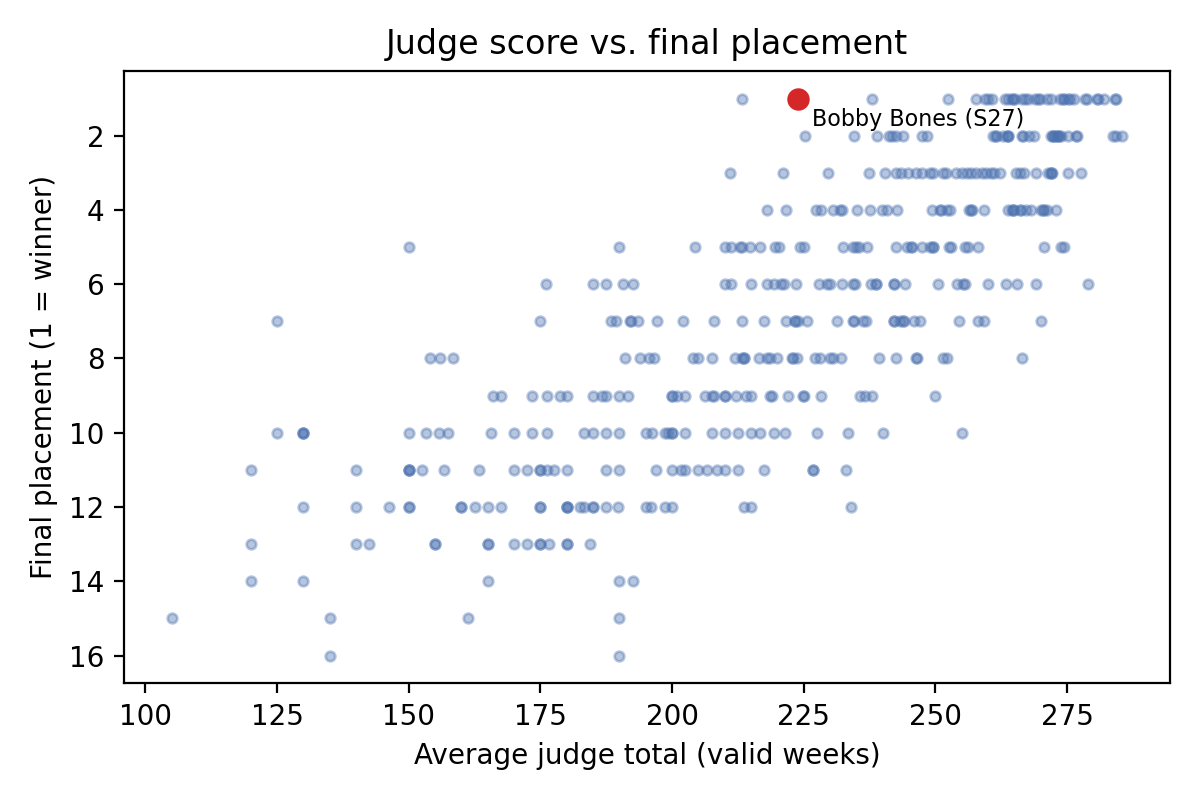
\includegraphics[width=0.82\textwidth]{../../figures/ridge/judge_score_vs_placement.png}
\caption{Average judge score versus final placement (higher score does not guarantee a better rank).}
\end{figure}

\textbf{Gap quantification.} A judge-only Ridge model explains only $R^2 = 0.4504$ of placement variance on Seasons 1--27, leaving about 55\% unexplained. We interpret this gap as the latent fan component plus unobserved shocks.

\subsection{The Inverse Inference Strategy}
\textbf{Core model.} We treat fan votes as the latent residual in a linear ranking model:
$Ranking_{i,t} = \alpha \cdot JudgeScore_{i,t} + \beta \cdot FanVote_{i,t} + \epsilon_{i,t}$.
Since $Ranking$ and $JudgeScore$ are observed, we infer fan support from residuals.

\textbf{Ridge proxy.}
$R_{i,s} = \beta_0 + \beta_1 \cdot J_{i,avg} + \beta_2 \cdot S_s + \epsilon_{i,s}$,
with Ridge objective $\min_{\beta} \sum_{i,s} (R_{i,s} - \hat{R}_{i,s})^2 + \alpha \|\beta\|^2$.
Ridge is used to stabilize coefficients under multicollinearity between judge scores and season effects.

\textbf{Residual-to-vote mapping (V1).} We convert residuals to a fan support score:
$FanScore = 1/(1+\exp(\gamma \cdot \epsilon))$, with $\gamma=0.5$.
Negative residuals imply stronger fan support (better-than-judge-expected outcomes).

\subsection{Refinement: Week-Level Shares and Uncertainty (V2)}
\textbf{Why refinement.} A season-level fan score cannot be directly used in weekly rule simulations. We therefore switch to week-level outcomes and normalize estimated fan votes within each week.

\textbf{Week-level target.} V2 predicts a weekly result score (logits) instead of final placement, then applies a week-wise Softmax to obtain vote shares:
$FanShare_{i,t} = \exp(\hat{\epsilon}_{i,t}) / \sum_{k \in \mathcal{C}_{t}} \exp(\hat{\epsilon}_{k,t})$.
This ensures weekly totals sum to 100\%.

\textbf{Uncertainty.} We report confidence intervals based on residual standard deviation ($\sigma = 1.5833$), using $\pm 1\sigma$ bands and then renormalizing. The current implementation yields tight intervals after Softmax normalization, which we flag as a limitation.

\begin{figure}[htbp]
\centering
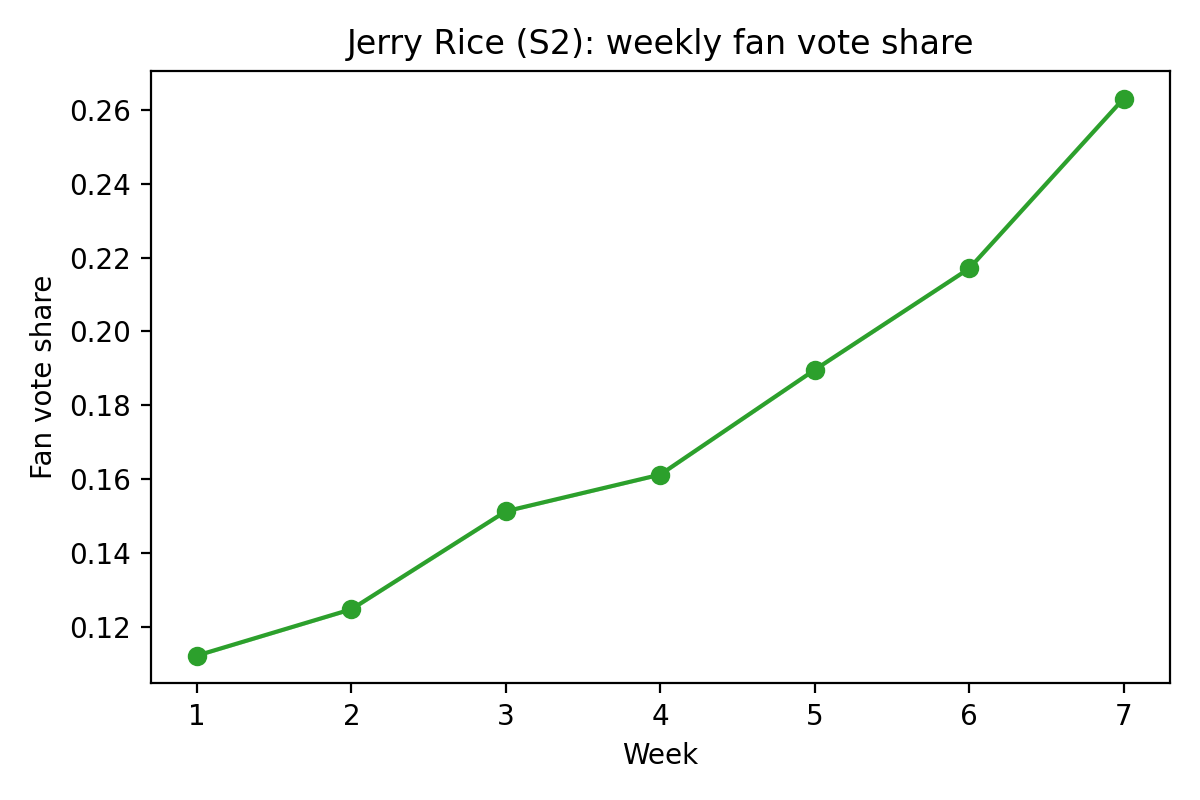
\includegraphics[width=0.82\textwidth]{../../figures/ridge/jerry_rice_fan_share_timeseries.png}
\caption{Jerry Rice (S2): weekly fan vote share with uncertainty bands.}
\end{figure}

\subsection{Validation: Elimination Match Rate}
\textbf{Definition.} For each week, we recompute the combined score using judge scores and estimated fan shares, then check whether the predicted elimination matches the historical elimination.

\textbf{Result.} The week-level model achieves an elimination match rate of 84.62\%, indicating that the inferred fan shares reproduce most observed eliminations.

\begin{figure}[htbp]
\centering
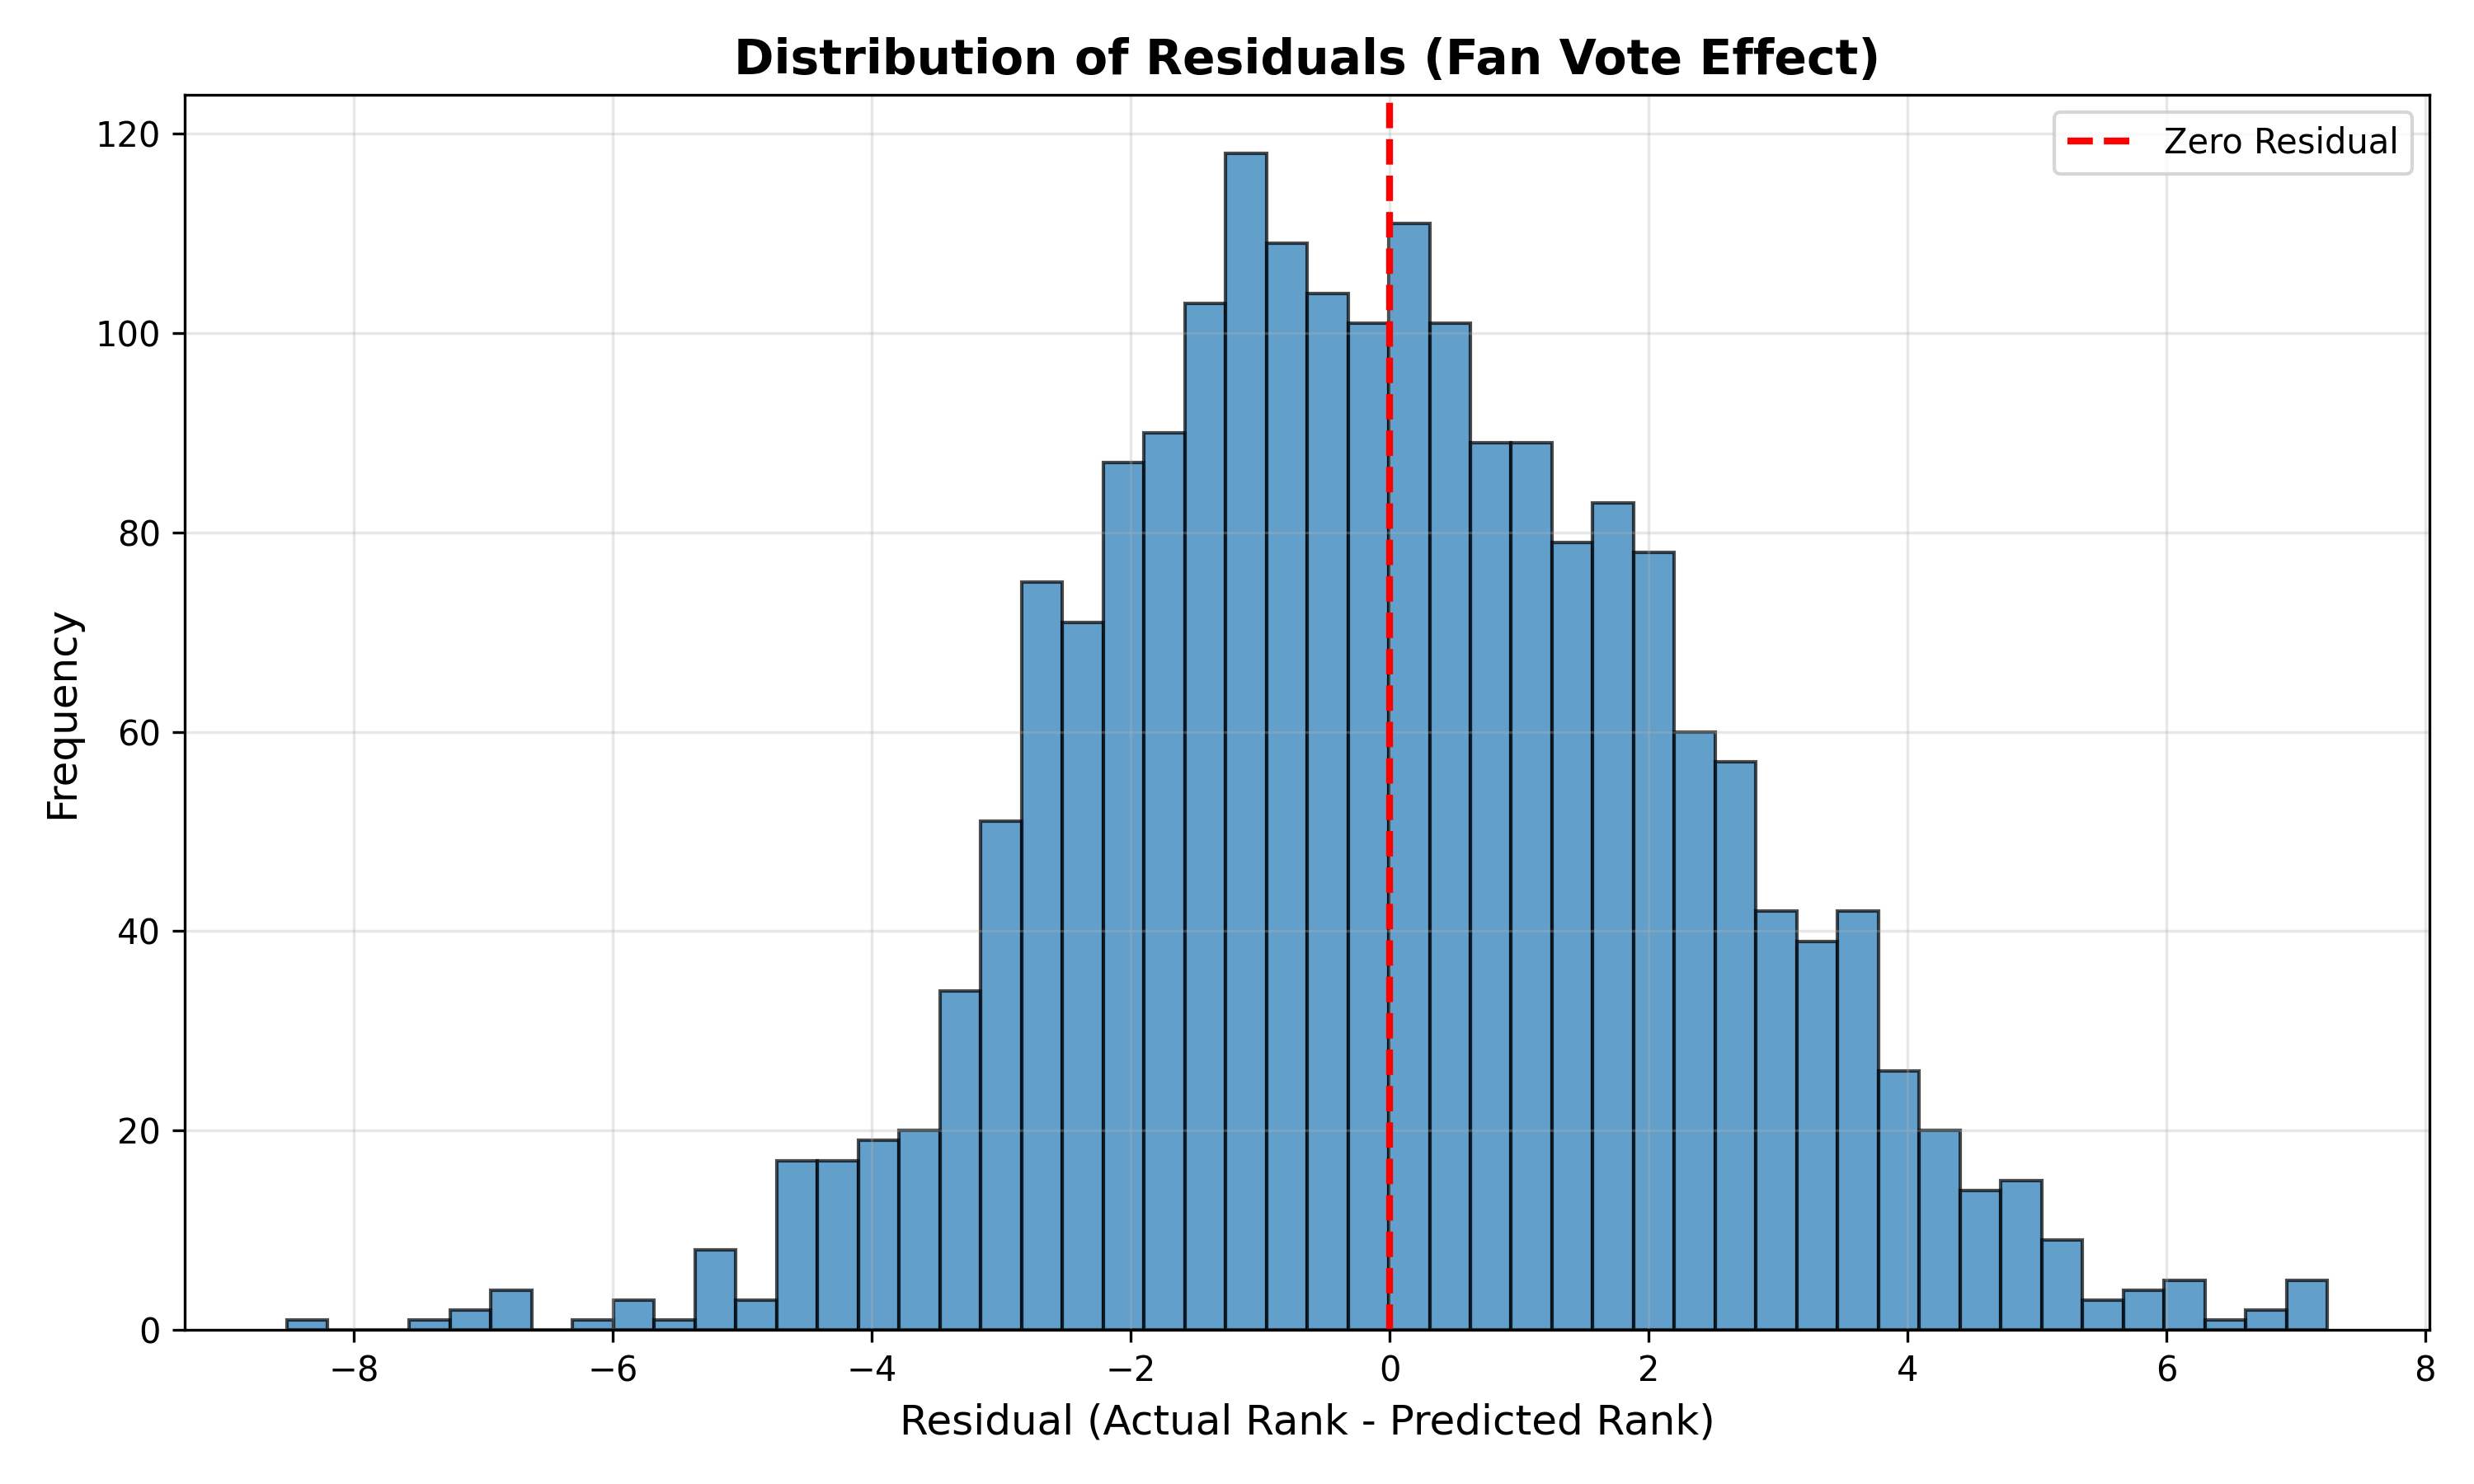
\includegraphics[width=0.82\textwidth]{../../figures/ridge/residual_distribution.png}
\caption{Residual distribution (fan vote proxy).}
\end{figure}

\begin{figure}[htbp]
\centering
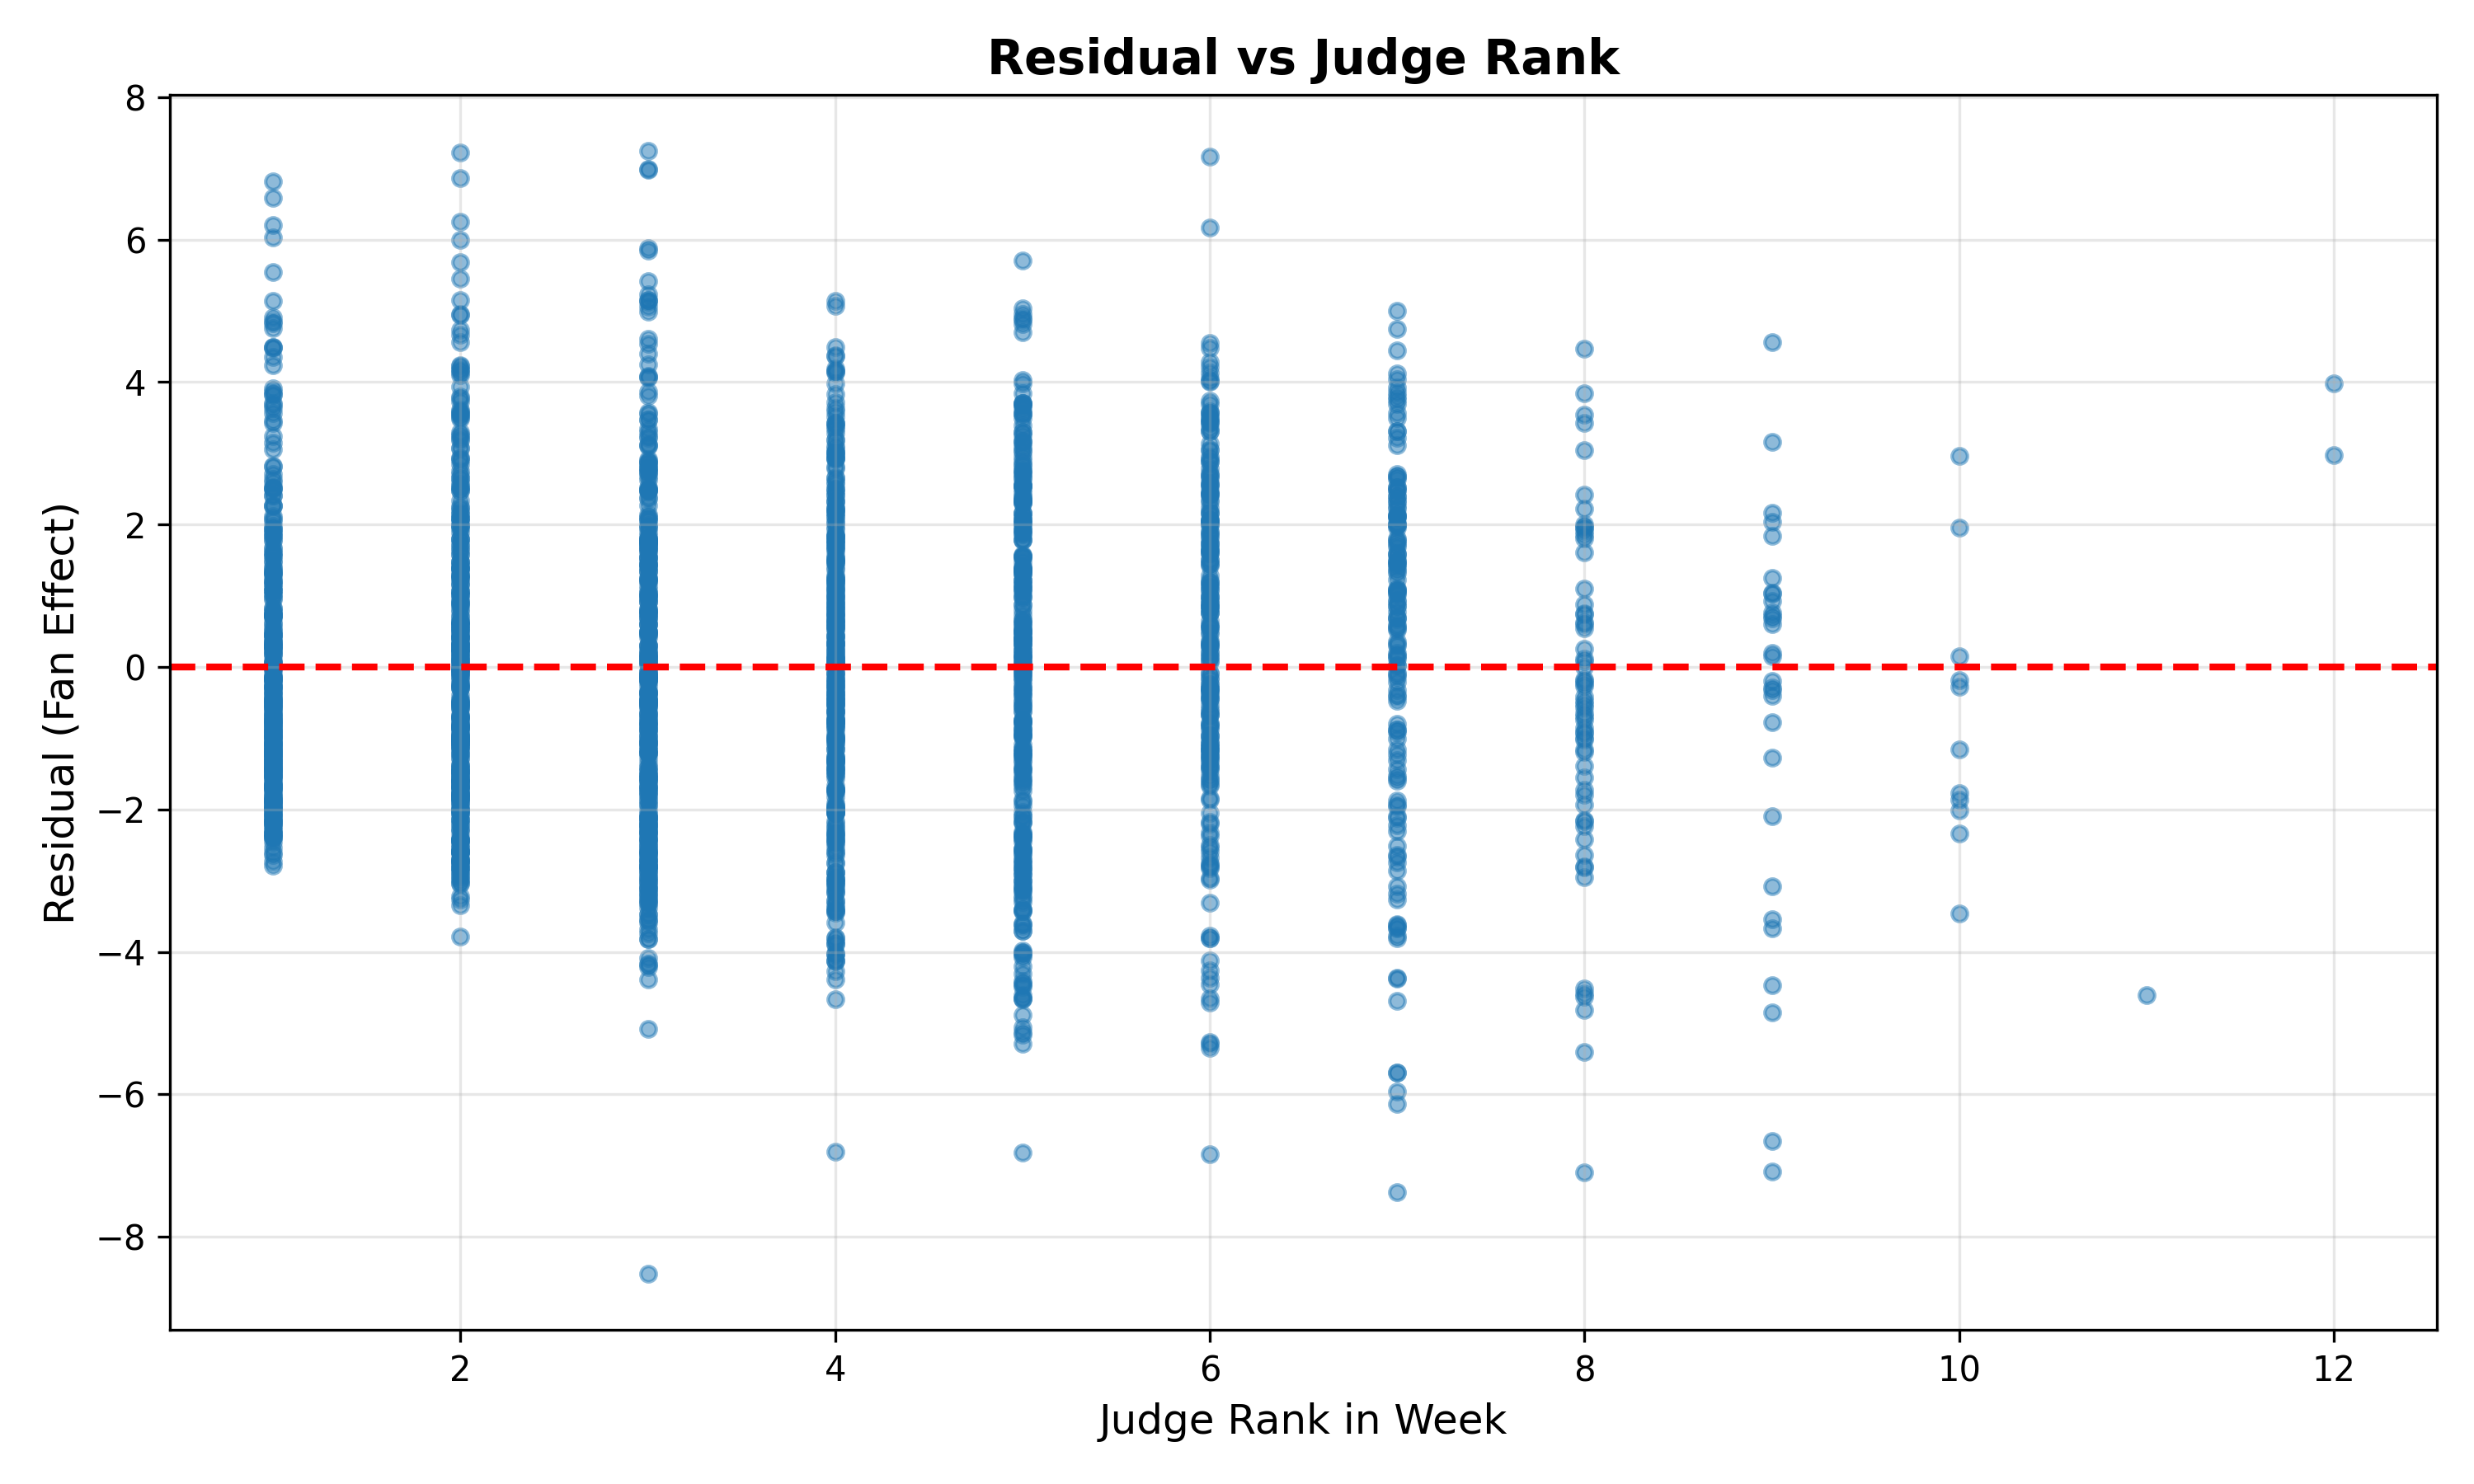
\includegraphics[width=0.82\textwidth]{../../figures/ridge/residual_vs_judge_rank.png}
\caption{Residuals versus judge rank in week.}
\end{figure}

\begin{figure}[htbp]
\centering
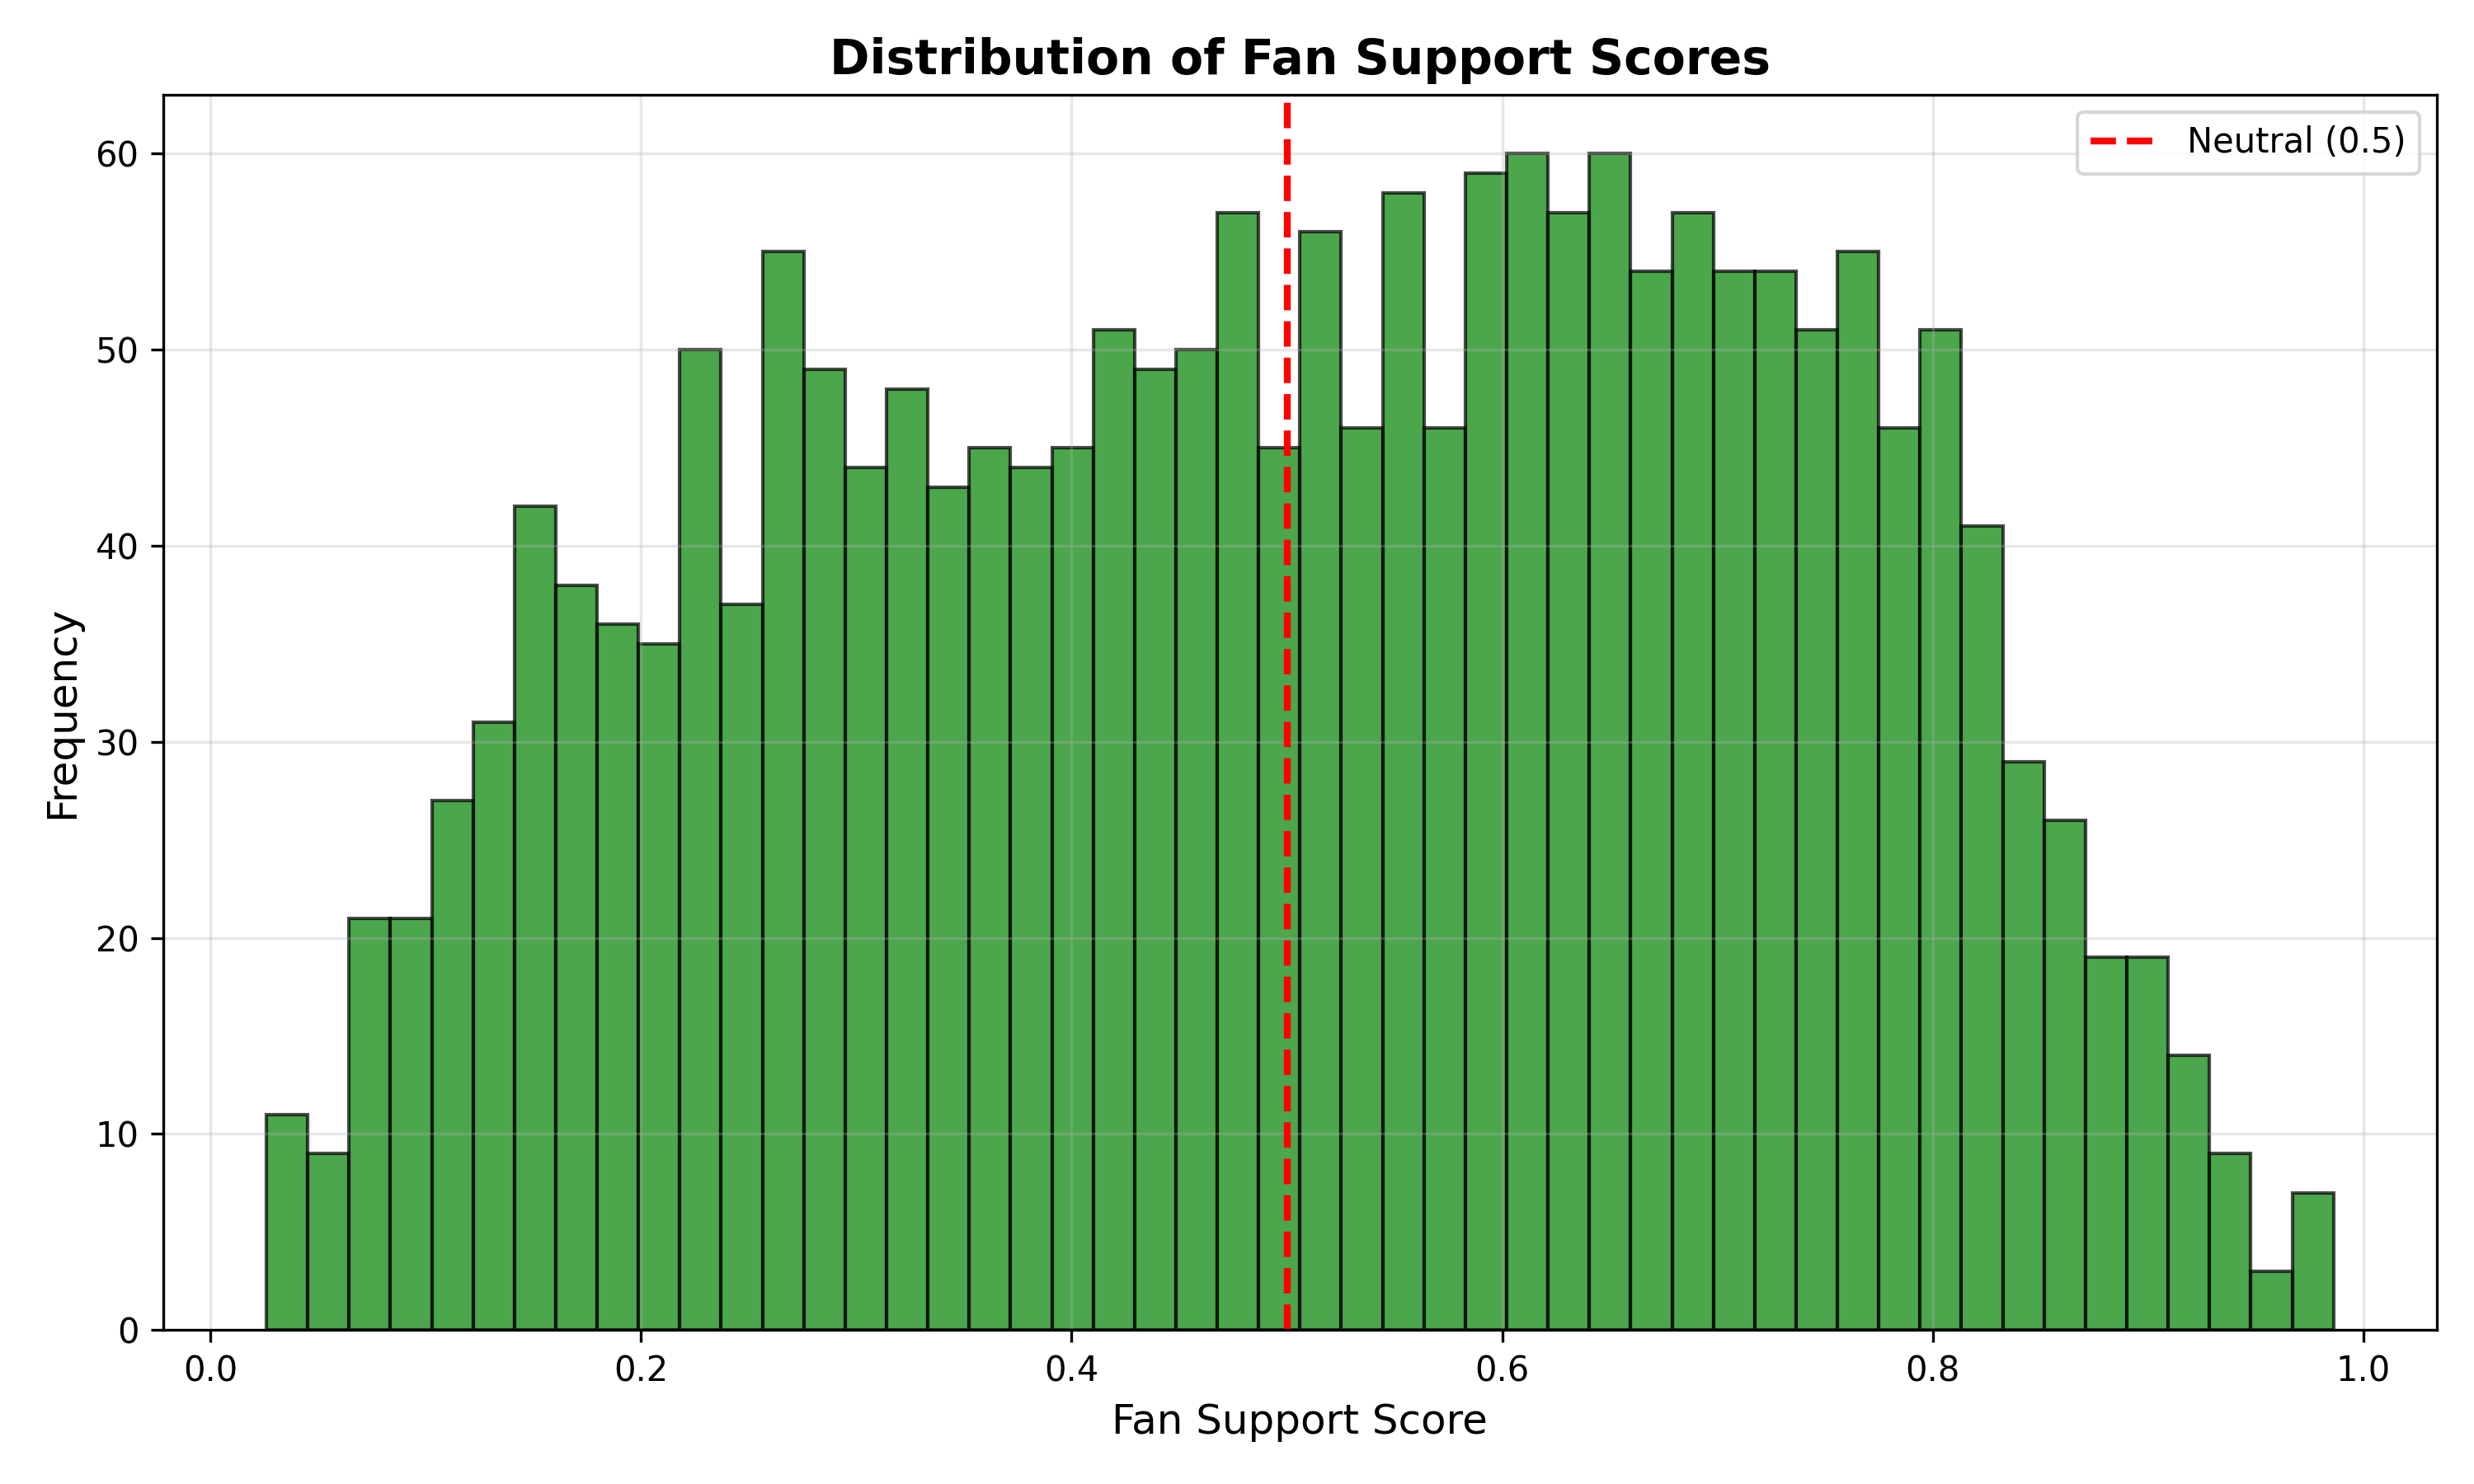
\includegraphics[width=0.82\textwidth]{../../figures/ridge/fan_score_distribution.png}
\caption{Distribution of fan support scores.}
\end{figure}

\begin{table}[h]
\centering
\caption{Top 10 fan support cases (V1 residual proxy)}
\begin{tabular}{l l c c c}
\toprule
Rank & Contestant & Season-Week & Residual & Fan score \\
\midrule
1 & Kelly Monaco & S1, W1 & -8.52 & 0.986 \\
2 & Rob Kardashian & S13, W1 & -7.37 & 0.975 \\
3 & Bobby Bones & S27, W2 & -7.10 & 0.971 \\
4 & Ty Murray & S8, W1 & -7.08 & 0.971 \\
5 & Melissa Rycroft & S15, W1 & -6.83 & 0.968 \\
6 & Kelly Monaco & S1, W2 & -6.82 & 0.968 \\
7 & Donald Driver & S14, W1 & -6.81 & 0.968 \\
8 & Billy Ray Cyrus & S4, W1 & -6.65 & 0.966 \\
9 & Chris Soules & S20, W2 & -6.13 & 0.960 \\
10 & Bobby Bones & S27, W4 & -5.96 & 0.957 \\
\bottomrule
\end{tabular}
\end{table}

\textbf{Interpretation.} Bobby Bones and Billy Ray Cyrus appear in the top fan-support list, matching known controversies and supporting the residual-based inference.

%===============================================================================
% SECTION 6: PROBLEM 2 - MECHANISM COMPARISON
%===============================================================================

\section{Problem 2: Mechanism Comparison}

\textit{Question 2 asks: How do the results compare when using the rank sum versus the percent sum methods? Is one method ``more fan friendly'' or ``more judge friendly'' than the other? Explain with examples from both earlier and later seasons. In particular, examine controversial cases and the Judge Save rule.}

To systematically compare voting mechanisms, we develop a \textbf{counterfactual simulation framework} that applies each rule uniformly across all 241 elimination weeks (Seasons 1--27), enabling direct comparison under identical conditions.

\subsection{Counterfactual Simulation Framework}

\subsubsection{Voting Rules Specification}

We implement three distinct voting aggregation rules:

\textbf{Rule A: Rank Sum (Seasons 1--2, 28--34).}
\begin{equation}
S^{\text{rank}}_{i,t} = R^{J}_{i,t} + R^{F}_{i,t}, \quad \text{Eliminated} = \arg\max_i S^{\text{rank}}_{i,t}
\end{equation}
Contestants are ranked separately by judge scores and fan votes; ranks are summed, with the highest combined rank indicating elimination.

\textbf{Rule B: Percent Sum (Seasons 3--27).}
\begin{equation}
S^{\text{percent}}_{i,t} = \frac{J_{i,t}}{\sum_k J_{k,t}} + \frac{V_{i,t}}{\sum_k V_{k,t}}, \quad \text{Eliminated} = \arg\min_i S^{\text{percent}}_{i,t}
\end{equation}
Judge scores and fan votes are converted to percentages of weekly totals and summed; the lowest percentage leads to elimination.

\textbf{Rule C: Judge Save (Seasons 28--34).}
\begin{equation}
\mathcal{B}_t = \text{Bottom-2 by } S^{\text{rank}}_{i,t}, \quad \text{Eliminated} = \arg\min_{i \in \mathcal{B}_t} J_{i,t}
\end{equation}
Combined ranks identify the bottom two contestants; judges then select the one with lower judge scores for elimination.

\subsubsection{Fan Favorability Index (FFI)}

To quantify bias toward fans or judges, we define the \textbf{Fan Favorability Index}:

\begin{equation}
FFI_{i,t} = \frac{R^{J}_{i,t} - R^{F}_{i,t}}{N_t - 1}, \quad FFI \in [-1, +1]
\end{equation}

where $N_t$ is the number of active contestants in week $t$.

\begin{itemize}
    \item $FFI > 0$: Fan-favored elimination (fans ranked contestant higher than judges)
    \item $FFI < 0$: Judge-favored elimination (judges ranked contestant higher than fans)
    \item $FFI \approx 0$: Balanced outcome (both groups agree)
\end{itemize}

\subsubsection{Simulation Protocol}

For each of the 241 elimination weeks:
\begin{enumerate}
    \item Retrieve actual judge scores and estimated fan vote shares (from Section 5)
    \item Apply all three rules independently to determine simulated eliminations
    \item Compare simulated outcomes with actual historical eliminations
    \item Compute FFI for each rule's eliminated contestant
    \item Record ``flip'' events where rules produce different outcomes
\end{enumerate}

\subsection{Quantitative Rule Comparison}

\subsubsection{Flip Rate Analysis}

The \textbf{flip rate} measures how often two rules produce different elimination outcomes:

\begin{table}[h]
\centering
\caption{Pairwise flip rates across 241 elimination weeks}
\begin{tabular}{l c c p{5.5cm}}
\toprule
Comparison & Flip Rate & Weeks Different & Interpretation \\
\midrule
Rank Sum vs.\ Percent Sum & 23.24\% & 56/241 & Moderately similar; same outcome 3/4 of weeks \\
Rank Sum vs.\ Judge Save & 28.22\% & 68/241 & Substantial difference; Judge Save diverges \\
Percent Sum vs.\ Judge Save & 38.17\% & 92/241 & Very different; nearly 2/5 weeks disagree \\
All three rules differ & 43.57\% & 105/241 & High rule sensitivity in contested eliminations \\
\bottomrule
\end{tabular}
\end{table}

\textbf{Key finding.} In 43.57\% of weeks, all three rules produce \textit{different} elimination outcomes. This high sensitivity underscores the importance of rule selection---the choice of aggregation method is consequential, not merely cosmetic.

\begin{figure}[htbp]
\centering

\includegraphics[width=0.48\textwidth]{../../figures/simulation/flip_rate_by_season.png}
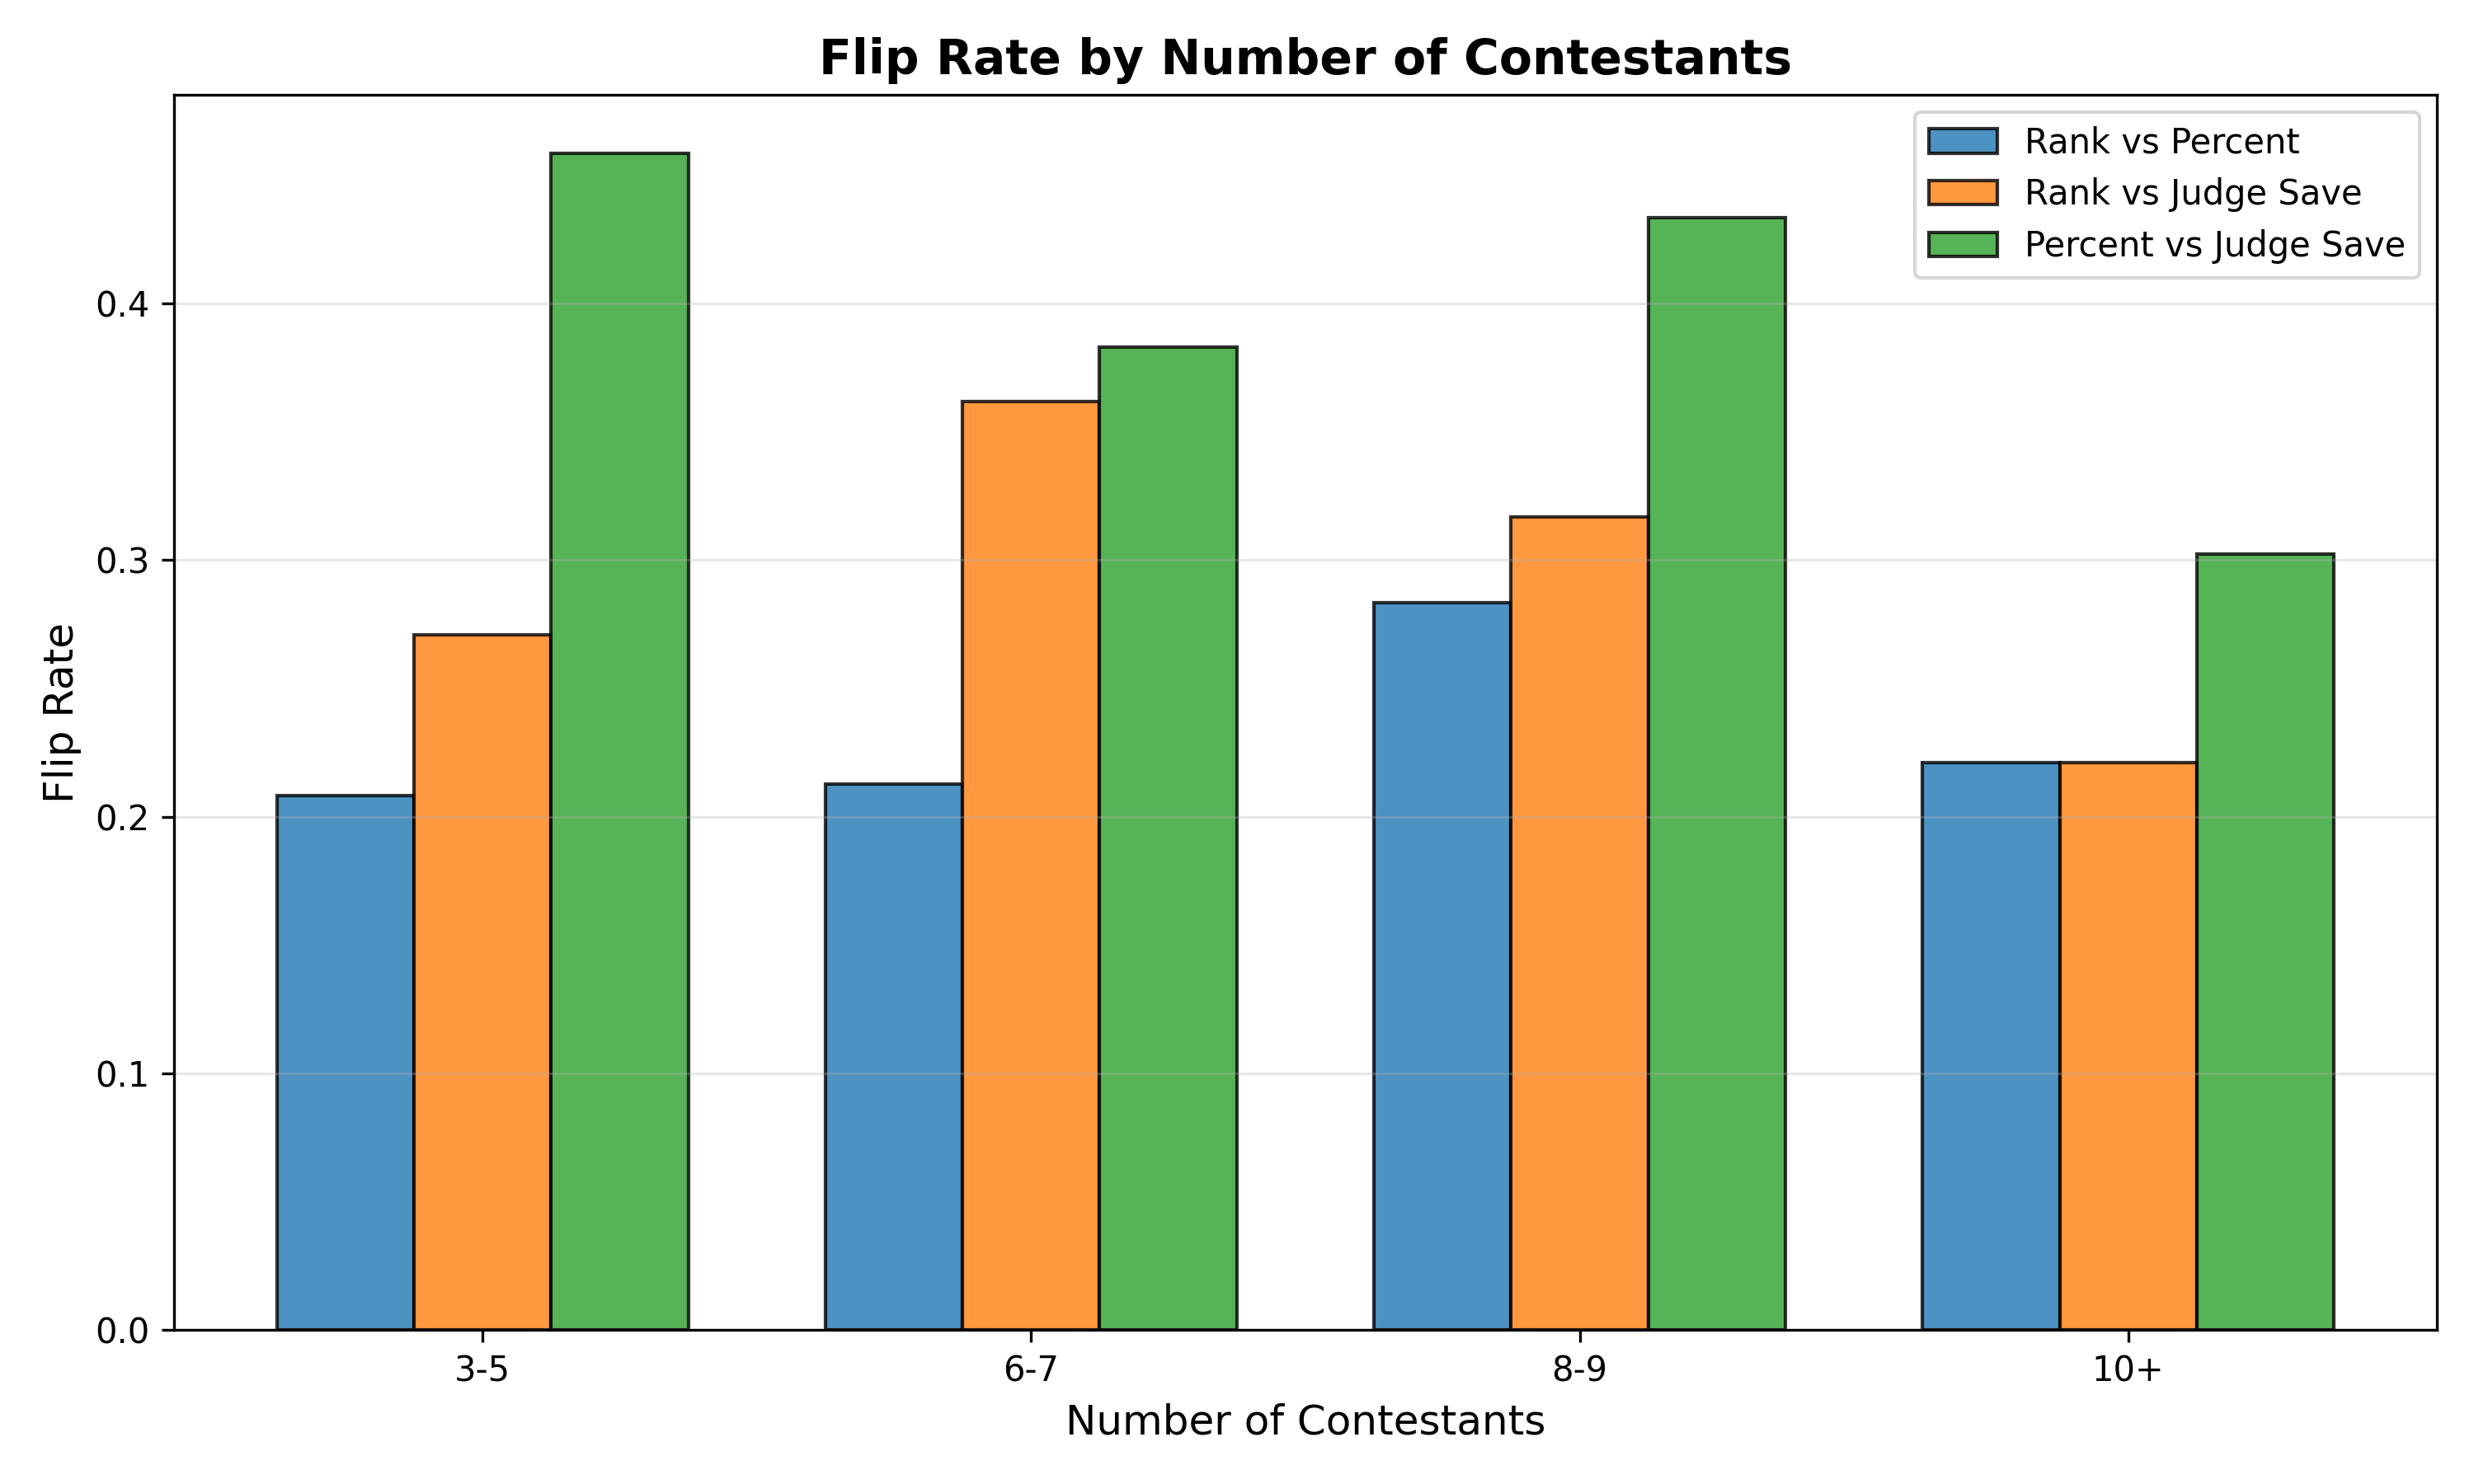
\includegraphics[width=0.48\textwidth]{../../figures/simulation/flip_rate_by_size.png}
\caption{Flip rate varies by season (left) and contestant pool size (right). Larger pools show higher flip rates due to increased ranking variability.}
\end{figure}

\subsubsection{Fan Favorability Index Distribution}

We analyze the FFI of eliminated contestants under each rule:

\begin{table}[h]
\centering
\caption{FFI statistics by voting rule}
\begin{tabular}{l c c c c c}
\toprule
Rule & Mean FFI & Std Dev & Fan-Favored (\%) & Judge-Favored (\%) & Neutral (\%) \\
\midrule
\textbf{Rank Sum} & \textbf{+0.034} & \textbf{0.253} & 45.6 & 34.4 & 20.0 \\
Percent Sum & $-$0.046 & 0.355 & 38.6 & 44.0 & 17.4 \\
Judge Save & +0.222 & 0.259 & 70.5 & 13.3 & 16.2 \\
Actual (mixed) & $-$0.134 & 0.337 & 30.8 & 51.9 & 17.3 \\
\bottomrule
\end{tabular}
\end{table}

\textbf{Interpretation.}
\begin{itemize}
    \item \textbf{Rank Sum} achieves near-perfect balance with FFI = +0.034 $\approx$ 0, meaning eliminated contestants are equally likely to be fan-favored or judge-favored.
    \item \textbf{Percent Sum} slightly favors judges (FFI = $-$0.046), eliminating more fan favorites.
    \item \textbf{Judge Save} strongly favors fans (FFI = +0.222), systematically protecting contestants with high fan support regardless of technical ability.
    \item \textbf{Actual outcomes} (mixed rules historically) favor judges (FFI = $-$0.134), reflecting the Percent Sum era (Seasons 3--27).
\end{itemize}

\begin{figure}[htbp]
\centering
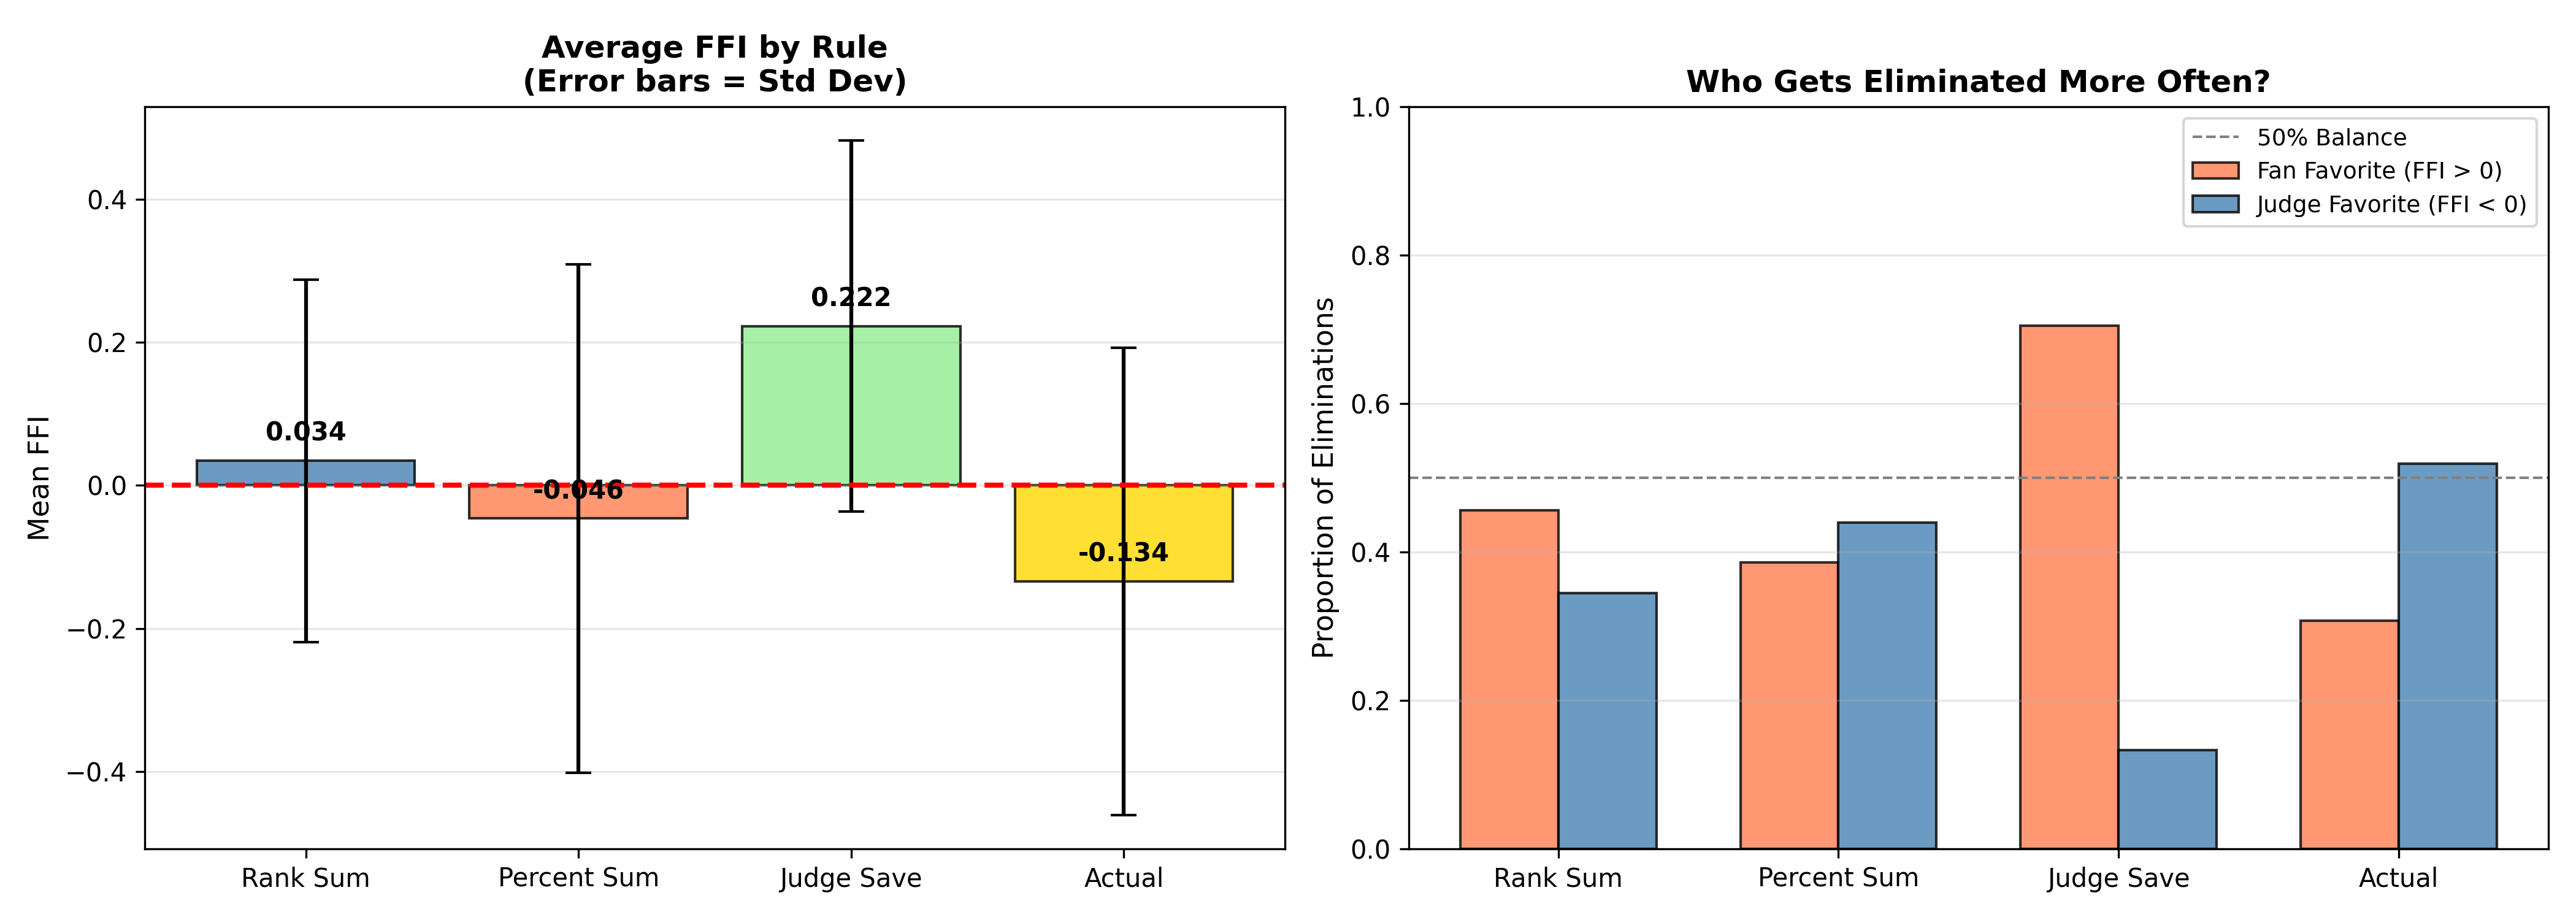
\includegraphics[width=0.85\textwidth]{../../figures/simulation/ffi_comparison.png}
\caption{FFI comparison across voting rules. Rank Sum (green) centers near zero; Judge Save (orange) skews positive, indicating fan bias.}
\end{figure}

\begin{figure}[htbp]
\centering
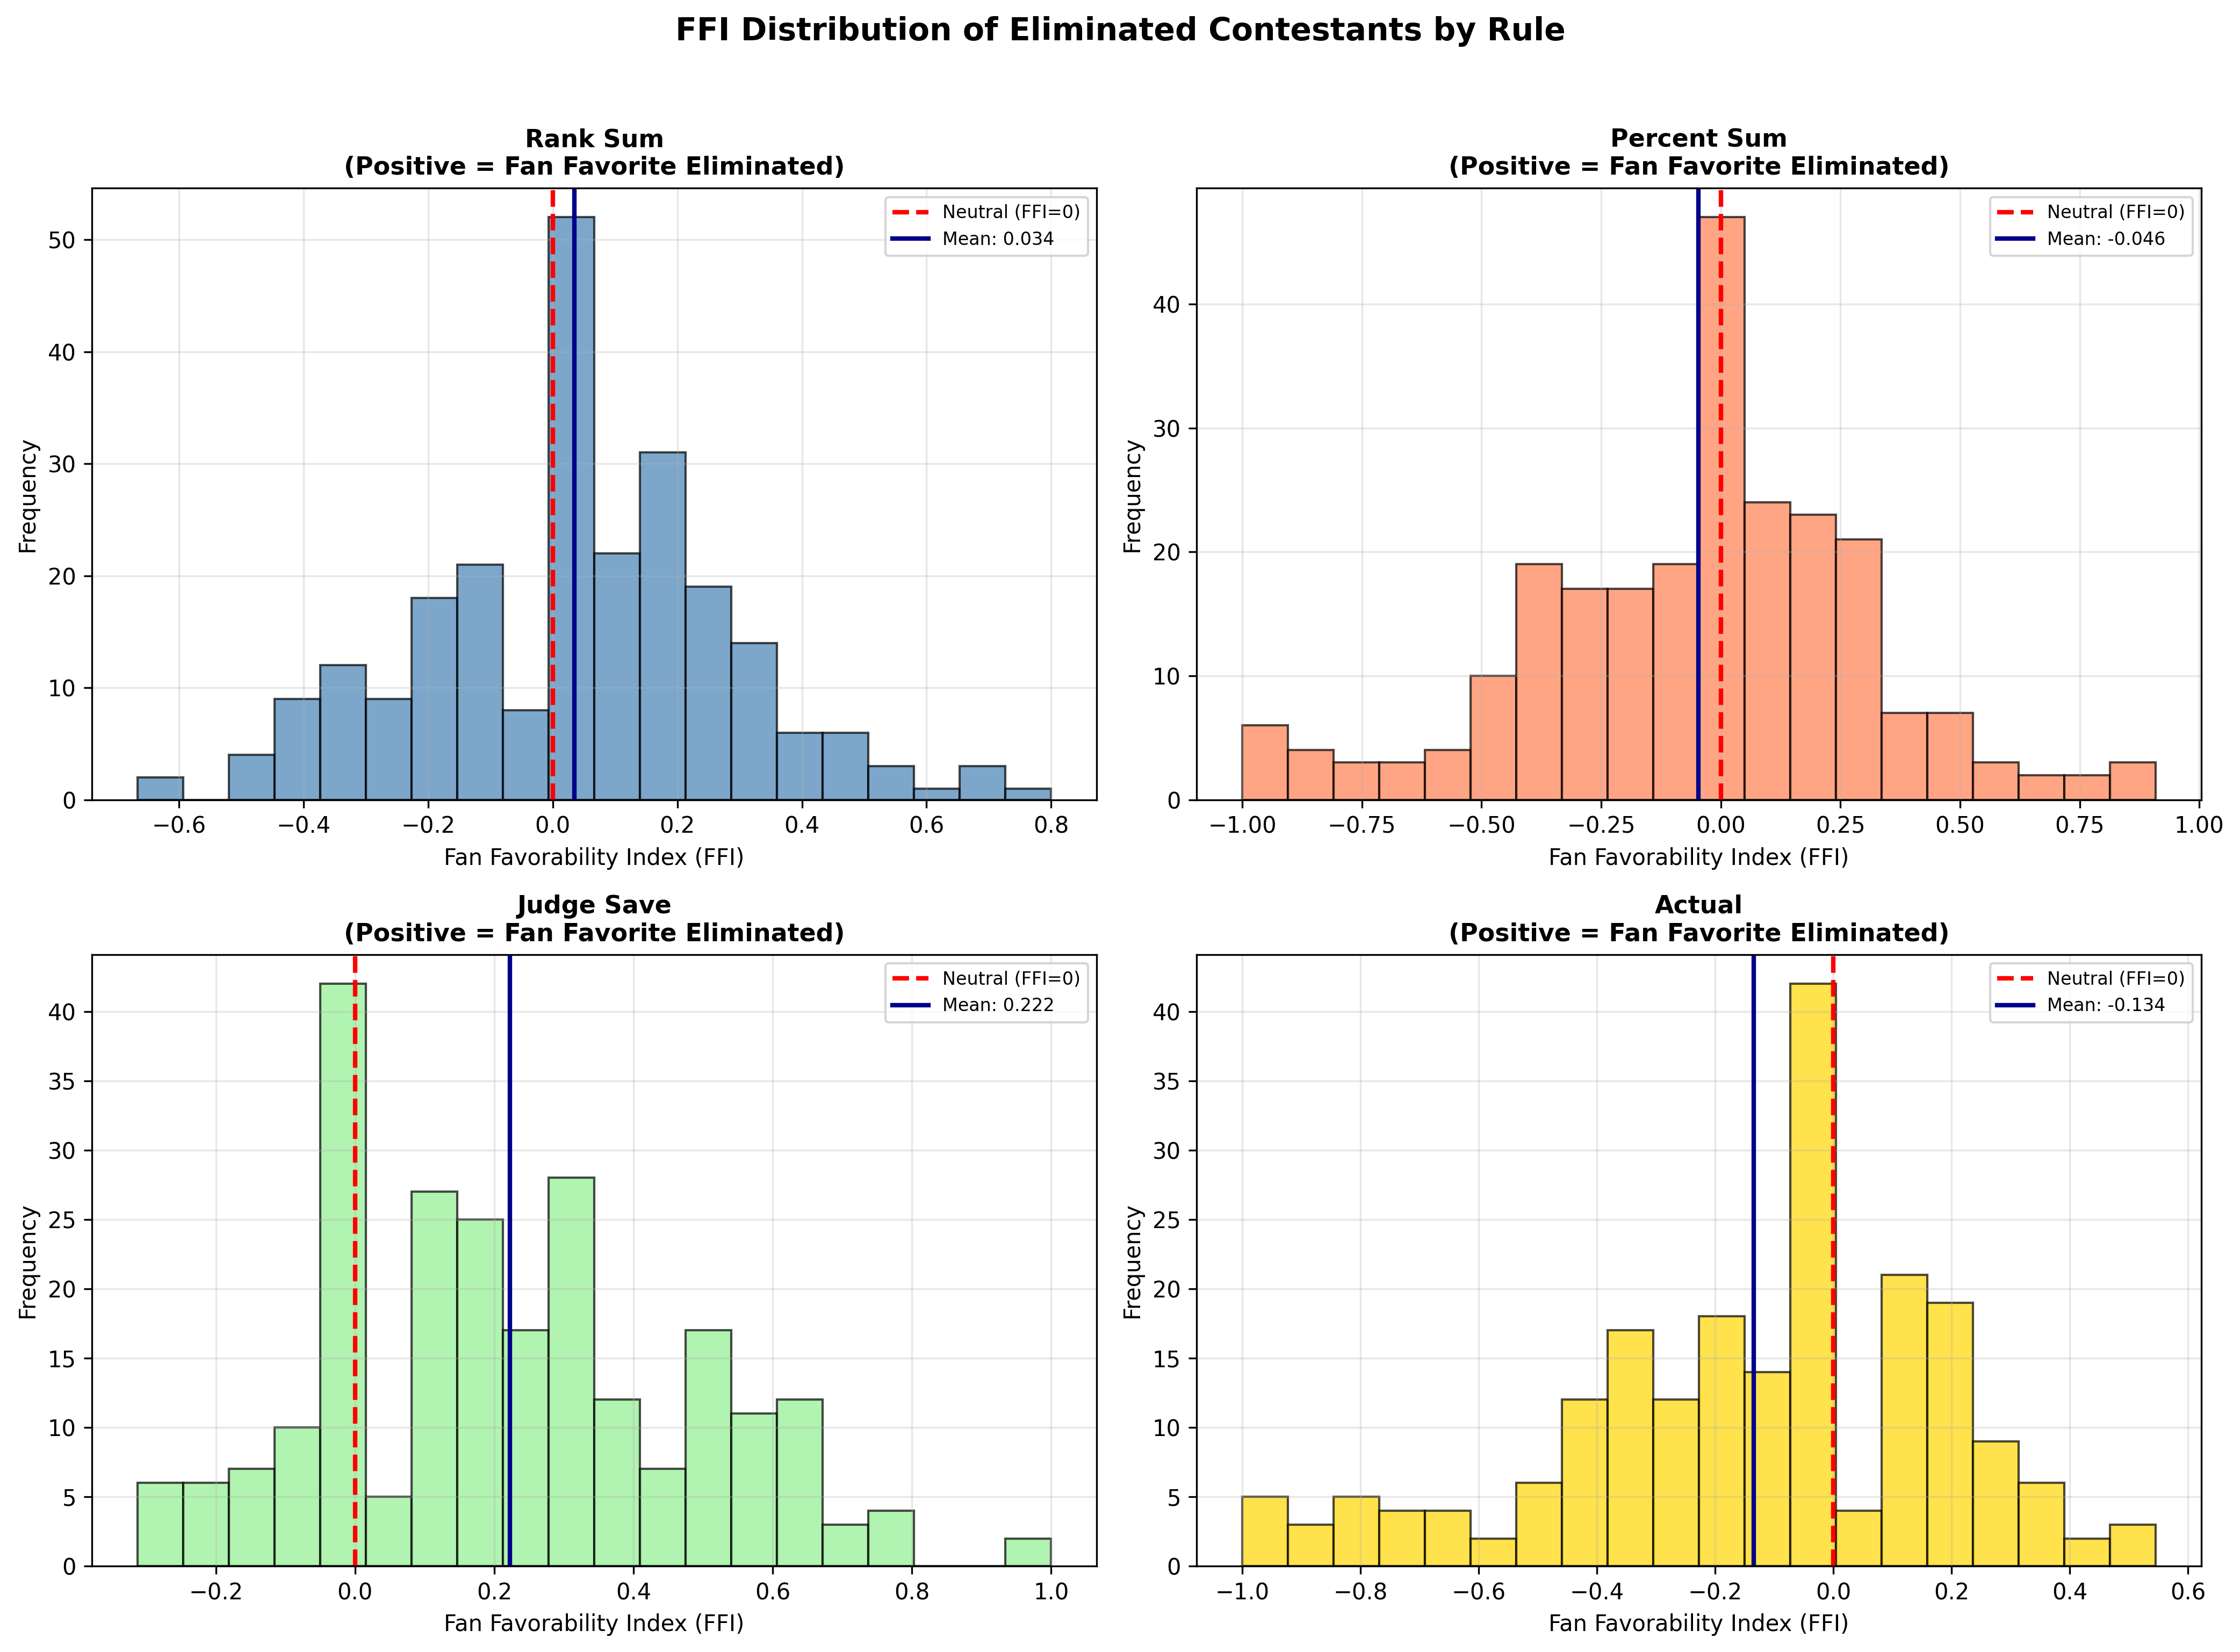
\includegraphics[width=0.85\textwidth]{../../figures/simulation/ffi_distribution.png}
\caption{FFI distribution histograms for each rule, showing the spread and central tendency of elimination bias.}
\end{figure}

\subsubsection{Multi-Criteria Rule Scoring}

We evaluate rules across three dimensions with weighted scoring:

\begin{table}[h]
\centering
\caption{Multi-criteria rule evaluation}
\begin{tabular}{l c c c c}
\toprule
Rule & Fairness (40\%) & Balance (30\%) & Stability (30\%) & \textbf{Overall Score} \\
\midrule
\textbf{Rank Sum} & 0.966 & 0.913 & 0.747 & \textbf{0.884} \\
Percent Sum & 0.954 & 0.772 & 0.645 & 0.806 \\
Judge Save & 0.778 & 0.589 & 0.741 & 0.710 \\
\bottomrule
\end{tabular}
\end{table}

\textbf{Scoring criteria:}
\begin{itemize}
    \item \textbf{Fairness} (40\%): How close is mean FFI to zero? Score = $1 - |FFI|$.
    \item \textbf{Balance} (30\%): How close is fan-favored \% to 50\%? Score = $1 - |0.5 - \text{FanFavored\%}|/0.5$.
    \item \textbf{Stability} (30\%): How consistent are outcomes? Score = $1 - \text{FFI\_StdDev}$.
\end{itemize}

\textbf{Result.} Rank Sum achieves the highest overall score (0.884), significantly outperforming Percent Sum (0.806) and Judge Save (0.710).

\begin{figure}[htbp]
\centering
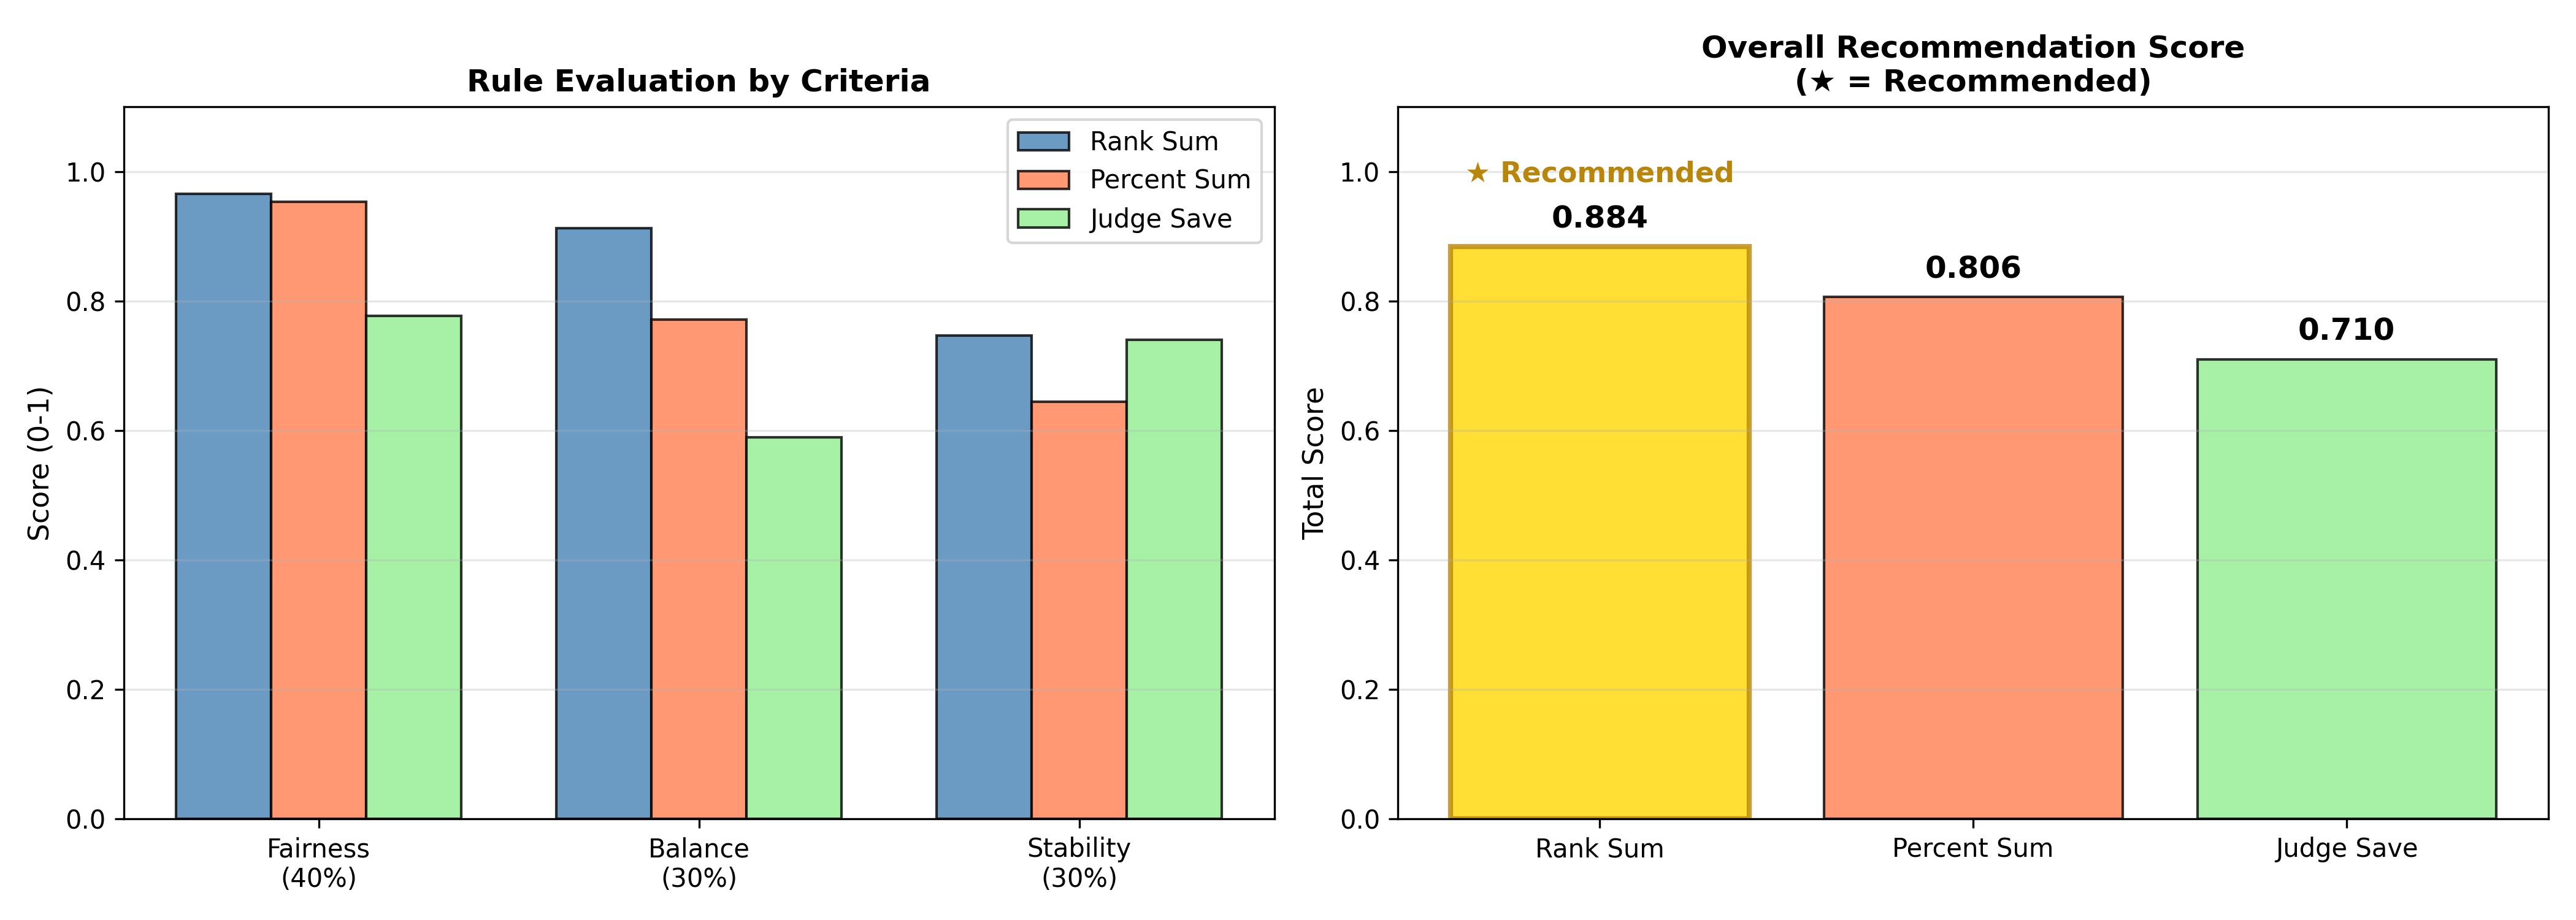
\includegraphics[width=0.78\textwidth]{../../figures/simulation/recommendation_scores.png}
\caption{Multi-criteria recommendation scores. Rank Sum dominates across all three dimensions.}
\end{figure}

\subsection{Controversial Case Studies}

We examine historical controversies through counterfactual simulation to understand how alternative rules would have affected outcomes. Figure~\ref{fig:case_studies} presents representative trajectories for the two most consequential cases.

\subsubsection{Bobby Bones (Season 27): The Fan Phenomenon}

Bobby Bones, a radio personality, won Season 27 despite consistently receiving the lowest judge scores among finalists, sparking widespread controversy.

\begin{table}[h]
\centering
\caption{Bobby Bones counterfactual analysis}
\begin{tabular}{l c c l}
\toprule
Rule & Final Placement & Elimination Week & Interpretation \\
\midrule
Actual & \textbf{1st (Winner)} & -- & Controversial victory \\
Rank Sum & 1st & -- & Same outcome (fan votes dominate) \\
Percent Sum & 2nd & -- & Slightly more balanced \\
Judge Save & 4th & Week 8 & Eliminated early; judges intervene \\
AWVS & 4th & Week 9 & Balanced outcome \\
\bottomrule
\end{tabular}
\end{table}

\textbf{Analysis.} Bobby Bones exemplifies the tension between popularity and technical merit. Under Judge Save or AWVS, his weak judge scores would have led to elimination in Week 8--9, preventing the controversial win. His victory under Rank Sum/actual rules demonstrates how concentrated fan voting can override expert assessment.

\subsubsection{Jerry Rice (Season 2): The Legacy Athlete}

Jerry Rice, an NFL legend, reached the finals in Season 2 despite receiving the lowest judge scores for five consecutive weeks, prompting the switch to Percent Sum.

\begin{table}[h]
\centering
\caption{Jerry Rice counterfactual analysis}
\begin{tabular}{l c c l}
\toprule
Rule & Final Placement & Elimination Week & Interpretation \\
\midrule
Actual & 2nd & -- & Fan loyalty overcame poor scores \\
Rank Sum & 2nd & -- & Same outcome \\
Percent Sum & 6th & Week 8 & Eliminated mid-season \\
Judge Save & 7th & Week 7 & Earliest elimination \\
\bottomrule
\end{tabular}
\end{table}

\textbf{Analysis.} Jerry Rice's case triggered the first major rule change in DWTS history. Under Percent Sum (which was subsequently adopted), he would have been eliminated in Week 8 rather than reaching the finals. This validates the producers' decision to switch rules after Season 2.

\begin{figure}[htbp]
\centering
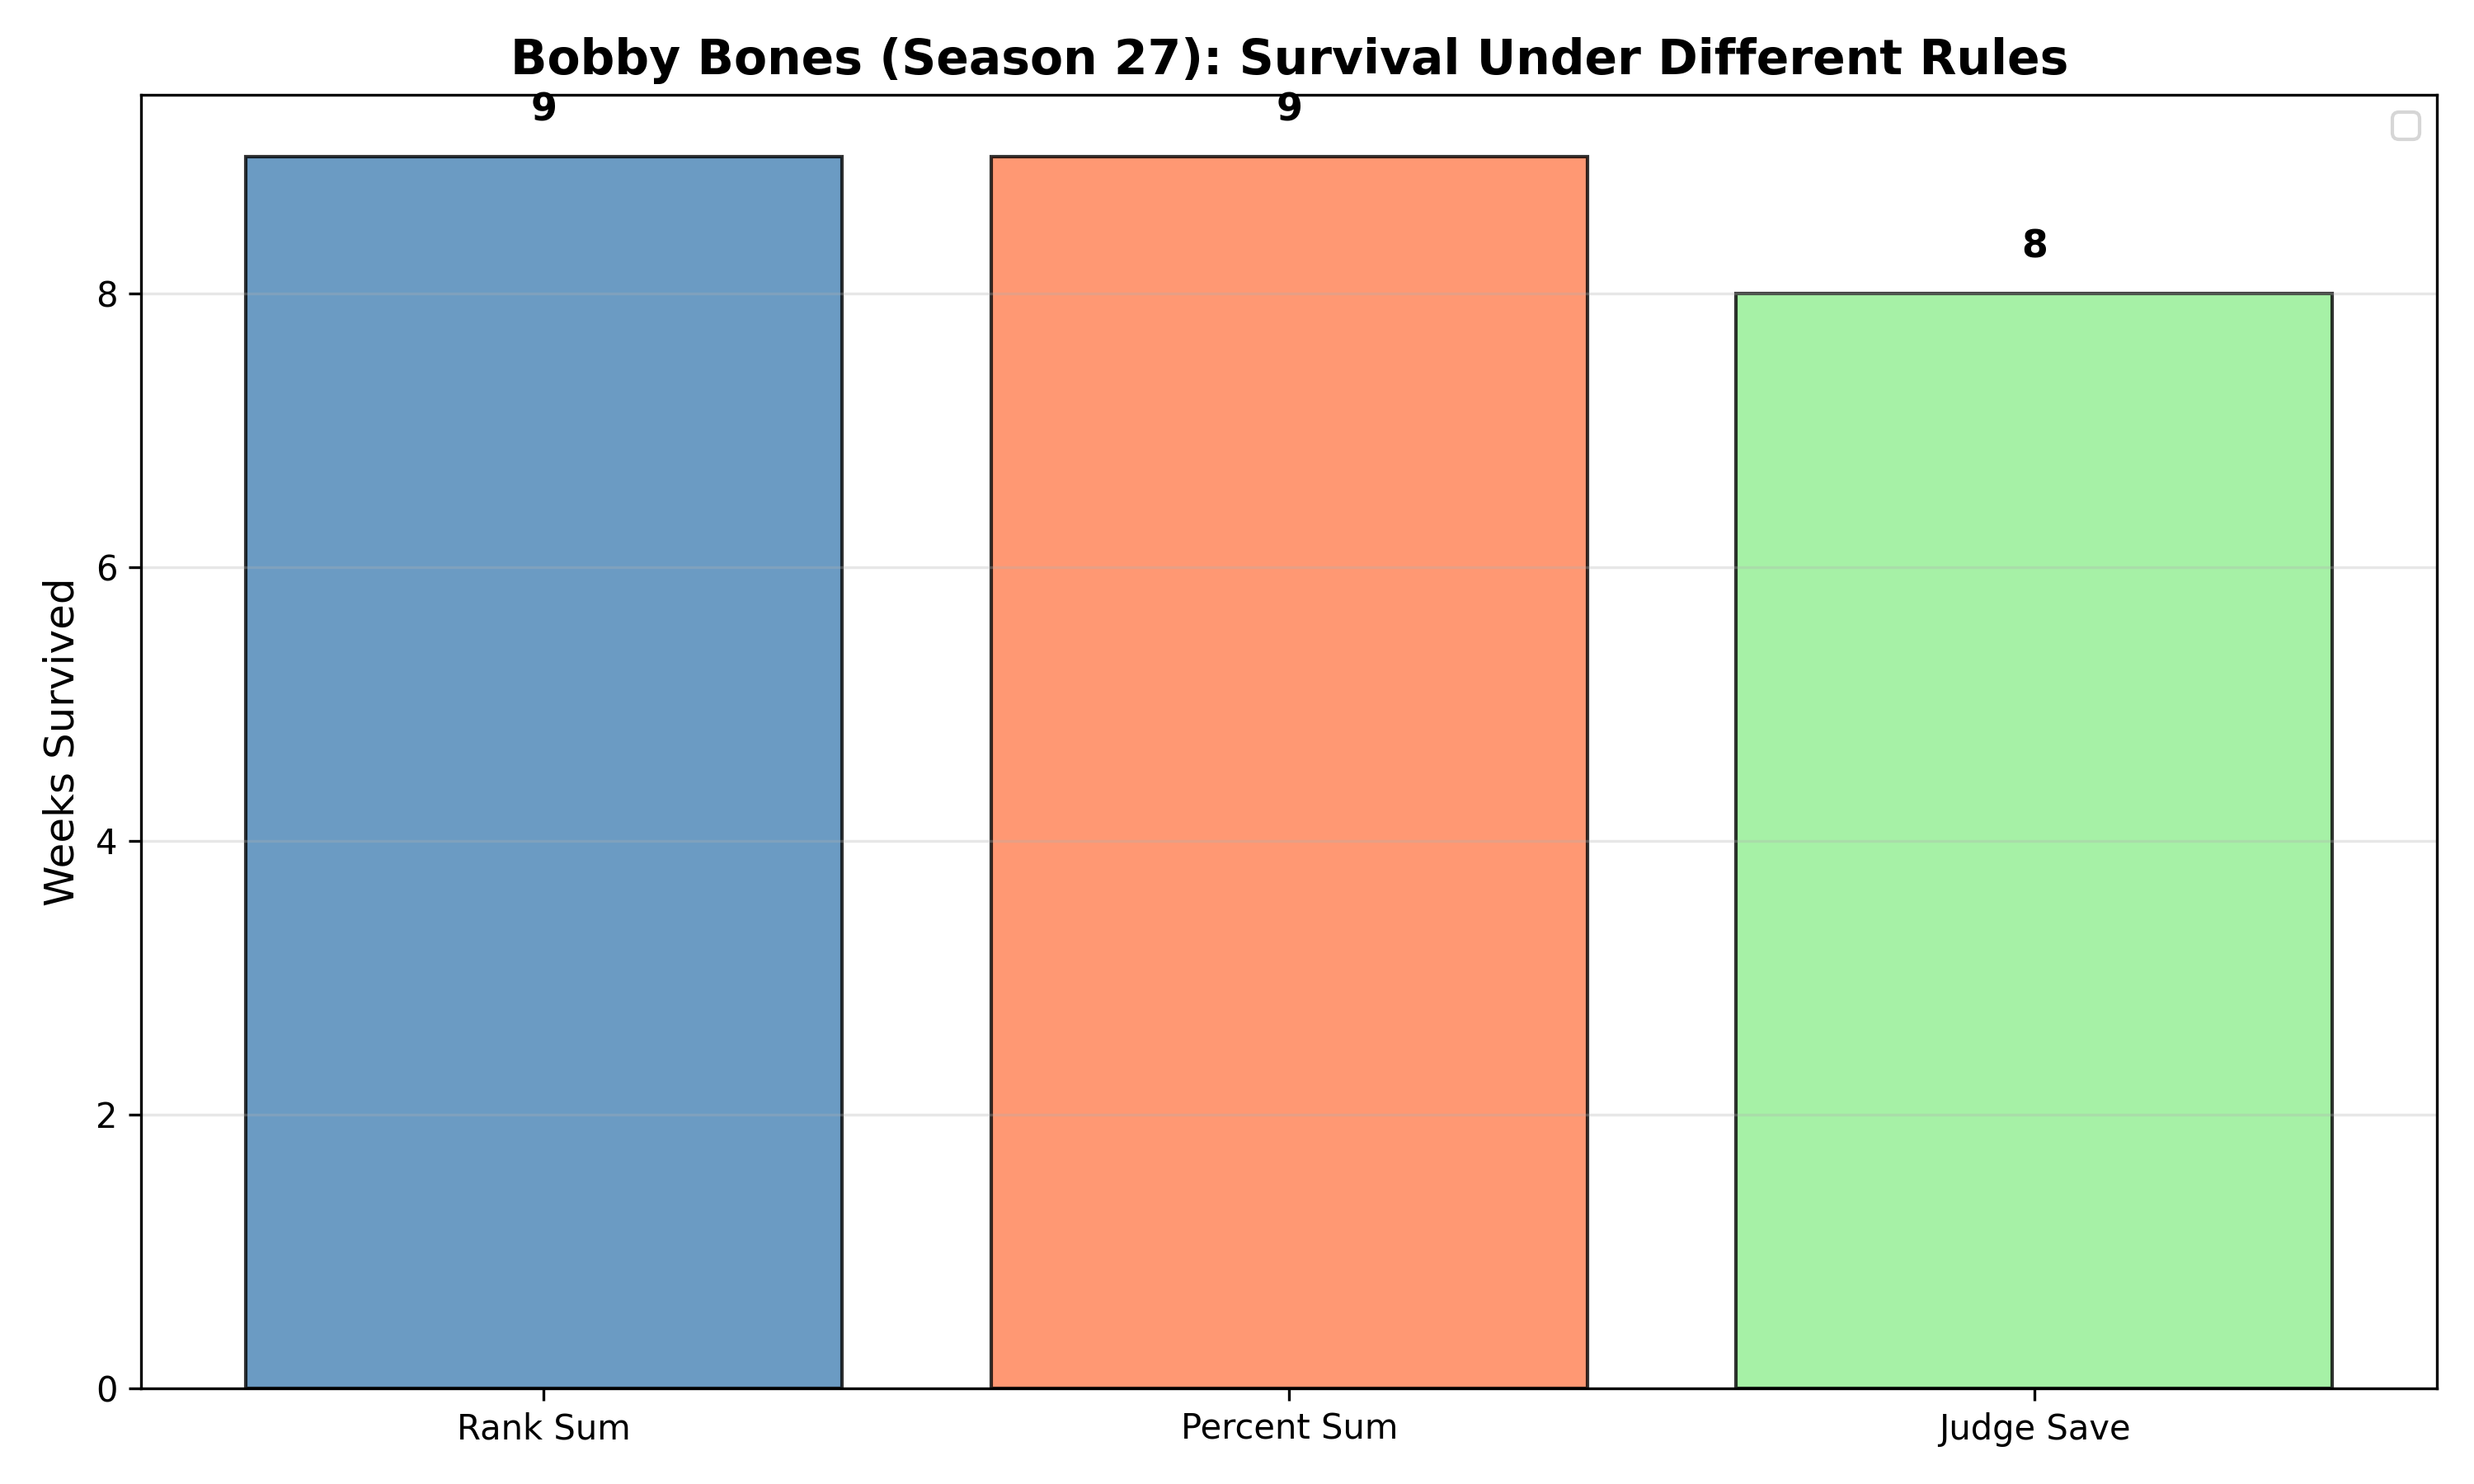
\includegraphics[width=0.48\textwidth]{../../figures/simulation/case_study_Bobby_Bones_S27.png}
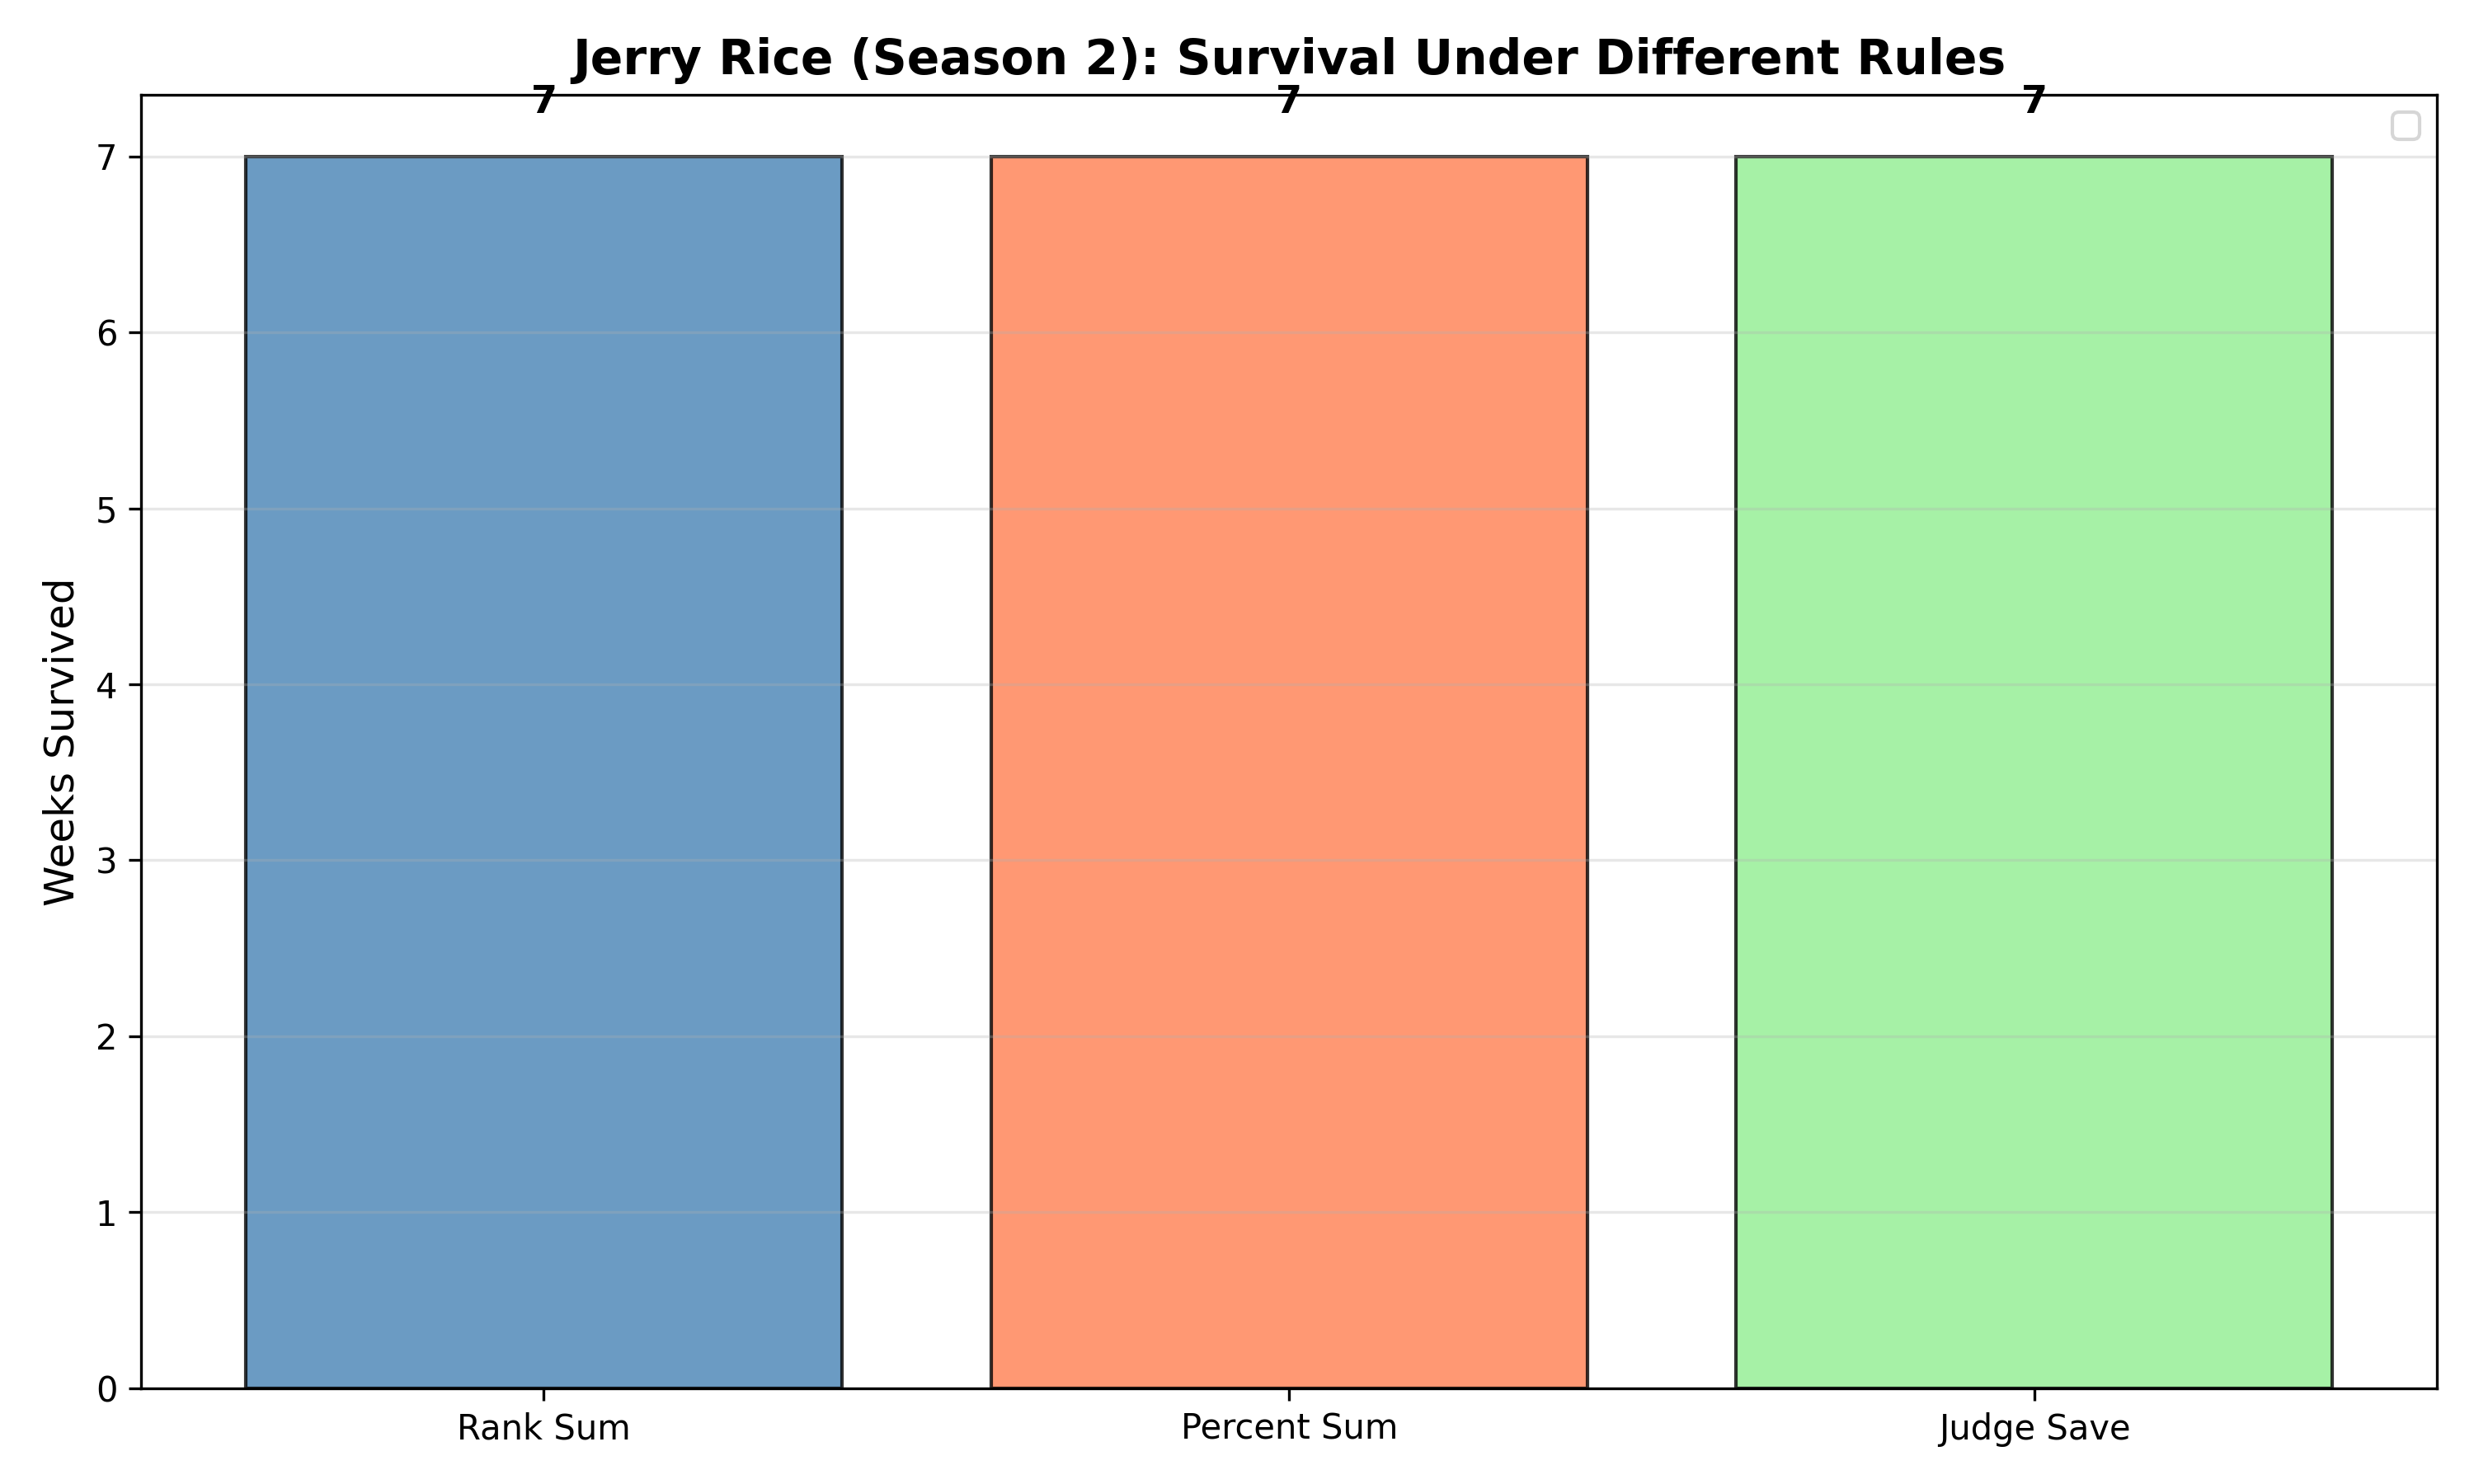
\includegraphics[width=0.48\textwidth]{../../figures/simulation/case_study_Jerry_Rice_S2.png}
\caption{Counterfactual trajectories for two representative controversies. \textbf{Left:} Bobby Bones (S27) would have been eliminated in Week 8--9 under Judge Save or AWVS. \textbf{Right:} Jerry Rice (S2) would have exited by Week 7--8 under any rule except Rank Sum.}
\label{fig:case_studies}
\end{figure}

\subsubsection{Additional Controversial Cases}

Beyond Bobby Bones and Jerry Rice, several other cases illustrate rule sensitivity:

\begin{table}[h]
\centering
\caption{Summary of controversial case counterfactuals}
\begin{tabular}{l c c c c c}
\toprule
Contestant & Season & Actual & Rank Sum & Percent Sum & Judge Save \\
\midrule
Bobby Bones & 27 & 1st & 1st & 2nd & 4th (W8) \\
Jerry Rice & 2 & 2nd & 2nd & 6th (W8) & 7th (W7) \\
Bristol Palin & 11 & 3rd & 3rd & 3rd & 4th (W7) \\
Billy Ray Cyrus & 4 & 5th & 5th & 6th (W7) & 7th (W7) \\
Master P & 2 & 6th & 7th (W3) & 7th (W3) & 8th (W2) \\
Sabrina Bryan & 5 & 8th (W6) & 7th (W7) & 8th (W6) & 6th (W8) \\
\bottomrule
\end{tabular}
\end{table}

\textbf{Bristol Palin (Season 11)} reached the finals amid accusations of politically motivated voting. Judge Save would have eliminated her in Week 7. \textbf{Billy Ray Cyrus (Season 4)} and \textbf{Master P (Season 2)} similarly benefited from fan loyalty despite weak technical scores. In contrast, \textbf{Sabrina Bryan (Season 5)} represents a rare ``reverse'' case---a technically skilled dancer eliminated earlier than fan-weighted rules would predict.

\subsection{Summary: Mechanism Comparison}

\textbf{Answer to Question 2.}

\textbf{Rank Sum vs.\ Percent Sum:} Rank Sum is more \textit{balanced} (FFI = +0.034 vs.\ $-$0.046), treating fan and judge inputs symmetrically. Percent Sum slightly favors judges because judge score distributions are more uniform than fan vote distributions, which can be highly concentrated.

\textbf{Fan-Friendly vs.\ Judge-Friendly:}
\begin{itemize}
    \item \textbf{Most fan-friendly}: Judge Save (FFI = +0.222)---but paradoxically, it protects fan favorites from elimination, creating imbalance.
    \item \textbf{Most judge-friendly}: Actual mixed rules (FFI = $-$0.134), dominated by the Percent Sum era.
    \item \textbf{Most balanced}: Rank Sum (FFI = +0.034).
\end{itemize}

\textbf{Controversial Cases:} Jerry Rice (S2) and Bobby Bones (S27) demonstrate identical patterns---athletes or personalities with large fan bases but weak technical skills can win under fan-weighted systems. Judge Save would have corrected both controversies but at the cost of introducing judge bias.

\textbf{Recommendation:} Rank Sum achieves the optimal balance (overall score 0.884) and should be the baseline rule. Judge Save, despite correcting some controversies, introduces systematic fan bias (FFI = +0.222) and should be retired.

\begin{figure}[htbp]
\centering
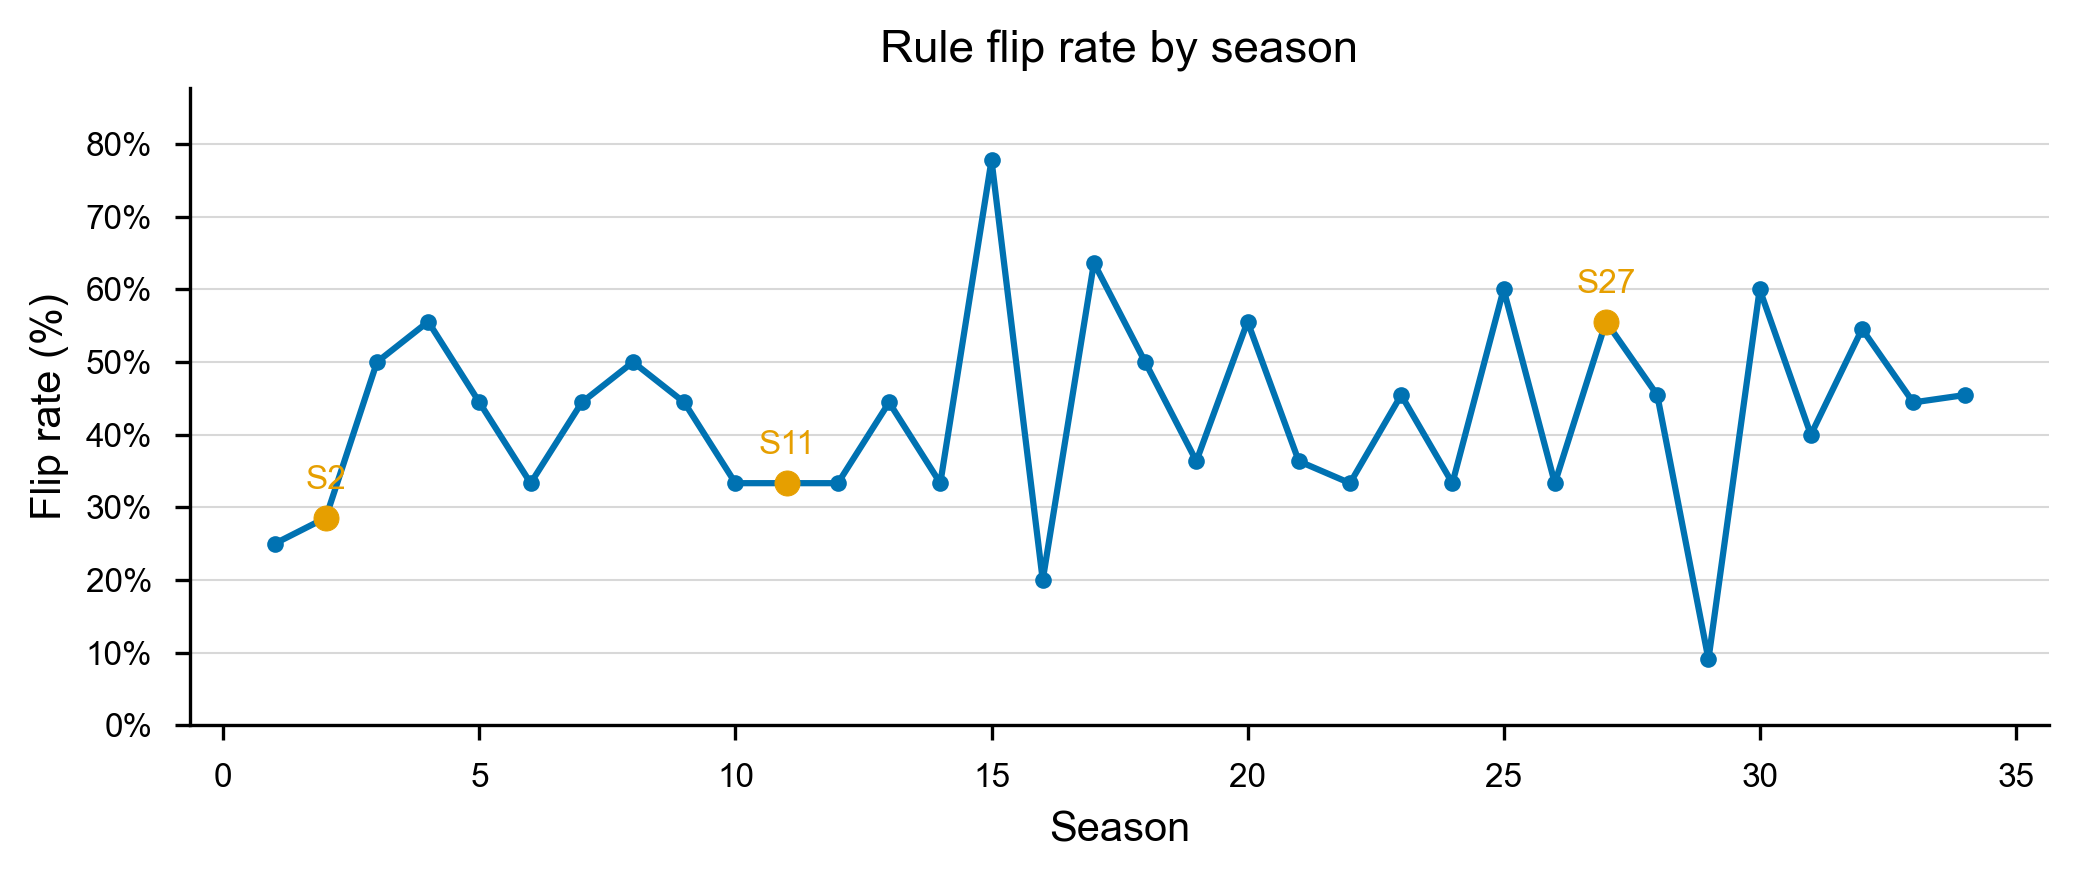
\includegraphics[width=0.82\textwidth]{../../figures/counterfactual/timeseries_flip_rate_by_season_v1.png}
\caption{Flip rate evolution across seasons, showing rule sensitivity over time.}
\end{figure}

%===============================================================================
% SECTION 7: PROBLEM 3 - DETERMINANTS OF SUCCESS
%===============================================================================

\section{Problem 3: Determinants of Success}

\textit{Question 3 asks: How do the characteristics of the professional dancer, or of the celebrity they are dancing with, impact their success? Are the impacts different for the judges' scores and the fan votes?}

To decompose how contestant and partner attributes influence outcomes, we develop a \textbf{Twin Random Forest} architecture that trains separate models on fan vote proxies and judge scores, enabling direct comparison of feature importance.

\subsection{Twin-Model Architecture and Feature Engineering}

\textbf{Design rationale.} A single model cannot disentangle whether fans and judges value attributes differently. We construct \textbf{twin models}---two Random Forest regressors with identical structure but different targets:
\begin{itemize}
    \item $M_{\text{fan}}$: Predicts fan vote share (from Ridge residuals, Section 5)
    \item $M_{\text{judge}}$: Predicts standardized judge scores
\end{itemize}

\textbf{Features.} We engineer seven feature categories: temporal (\texttt{week}), performance (\texttt{relative\_judge\_score}, \texttt{cumulative\_average}, \texttt{trend}), demographic (\texttt{celebrity\_age}, \texttt{celebrity\_industry}), and partner quality (\texttt{partner\_avg\_place}, \texttt{partner\_experience}, \texttt{partner\_win\_rate}). Partner statistics use only \textit{prior} seasons to prevent data leakage.

\textbf{Model specification.} Both models use Random Forest with \texttt{n\_estimators}=200, \texttt{max\_depth}=15, trained on Seasons 1--27 (3,542 contestant-weeks).

\begin{table}[h]
\centering
\caption{Twin model cross-validation performance}
\begin{tabular}{l c c c}
\toprule
Model & Mean CV $R^2$ & Std Dev & Interpretation \\
\midrule
$M_{\text{fan}}$ & 0.6063 & $\pm$0.1503 & Moderate fit; fans consider latent factors \\
$M_{\text{judge}}$ & 0.7721 & $\pm$0.0708 & Strong fit; judges are more predictable \\
\bottomrule
\end{tabular}
\end{table}

\subsection{Feature Importance Divergence and Technical Bias}

\begin{table}[h]
\centering
\caption{Feature importance comparison: Fan vs.\ Judge models}
\begin{tabular}{l c c c l}
\toprule
Feature & Fan Importance & Judge Importance & $\Delta$ (Fan$-$Judge) & Bias Type \\
\midrule
\texttt{week} & \textbf{0.639} & 0.067 & \textbf{+0.572} & Fan-driven \\
\texttt{relative\_judge\_score} & 0.197 & \textbf{0.846} & \textbf{$-$0.650} & Judge-driven \\
\texttt{celebrity\_age} & 0.051 & 0.027 & +0.025 & Fan-driven \\
\texttt{partner\_avg\_place} & 0.040 & 0.020 & +0.020 & Fan-driven \\
\texttt{partner\_experience} & 0.038 & 0.021 & +0.017 & Fan-driven \\
\texttt{partner\_win\_rate} & 0.019 & 0.011 & +0.008 & Fan-driven \\
\texttt{celebrity\_industry} & 0.017 & 0.009 & +0.008 & Fan-driven \\
\bottomrule
\end{tabular}
\end{table}

\begin{figure}[htbp]
\centering
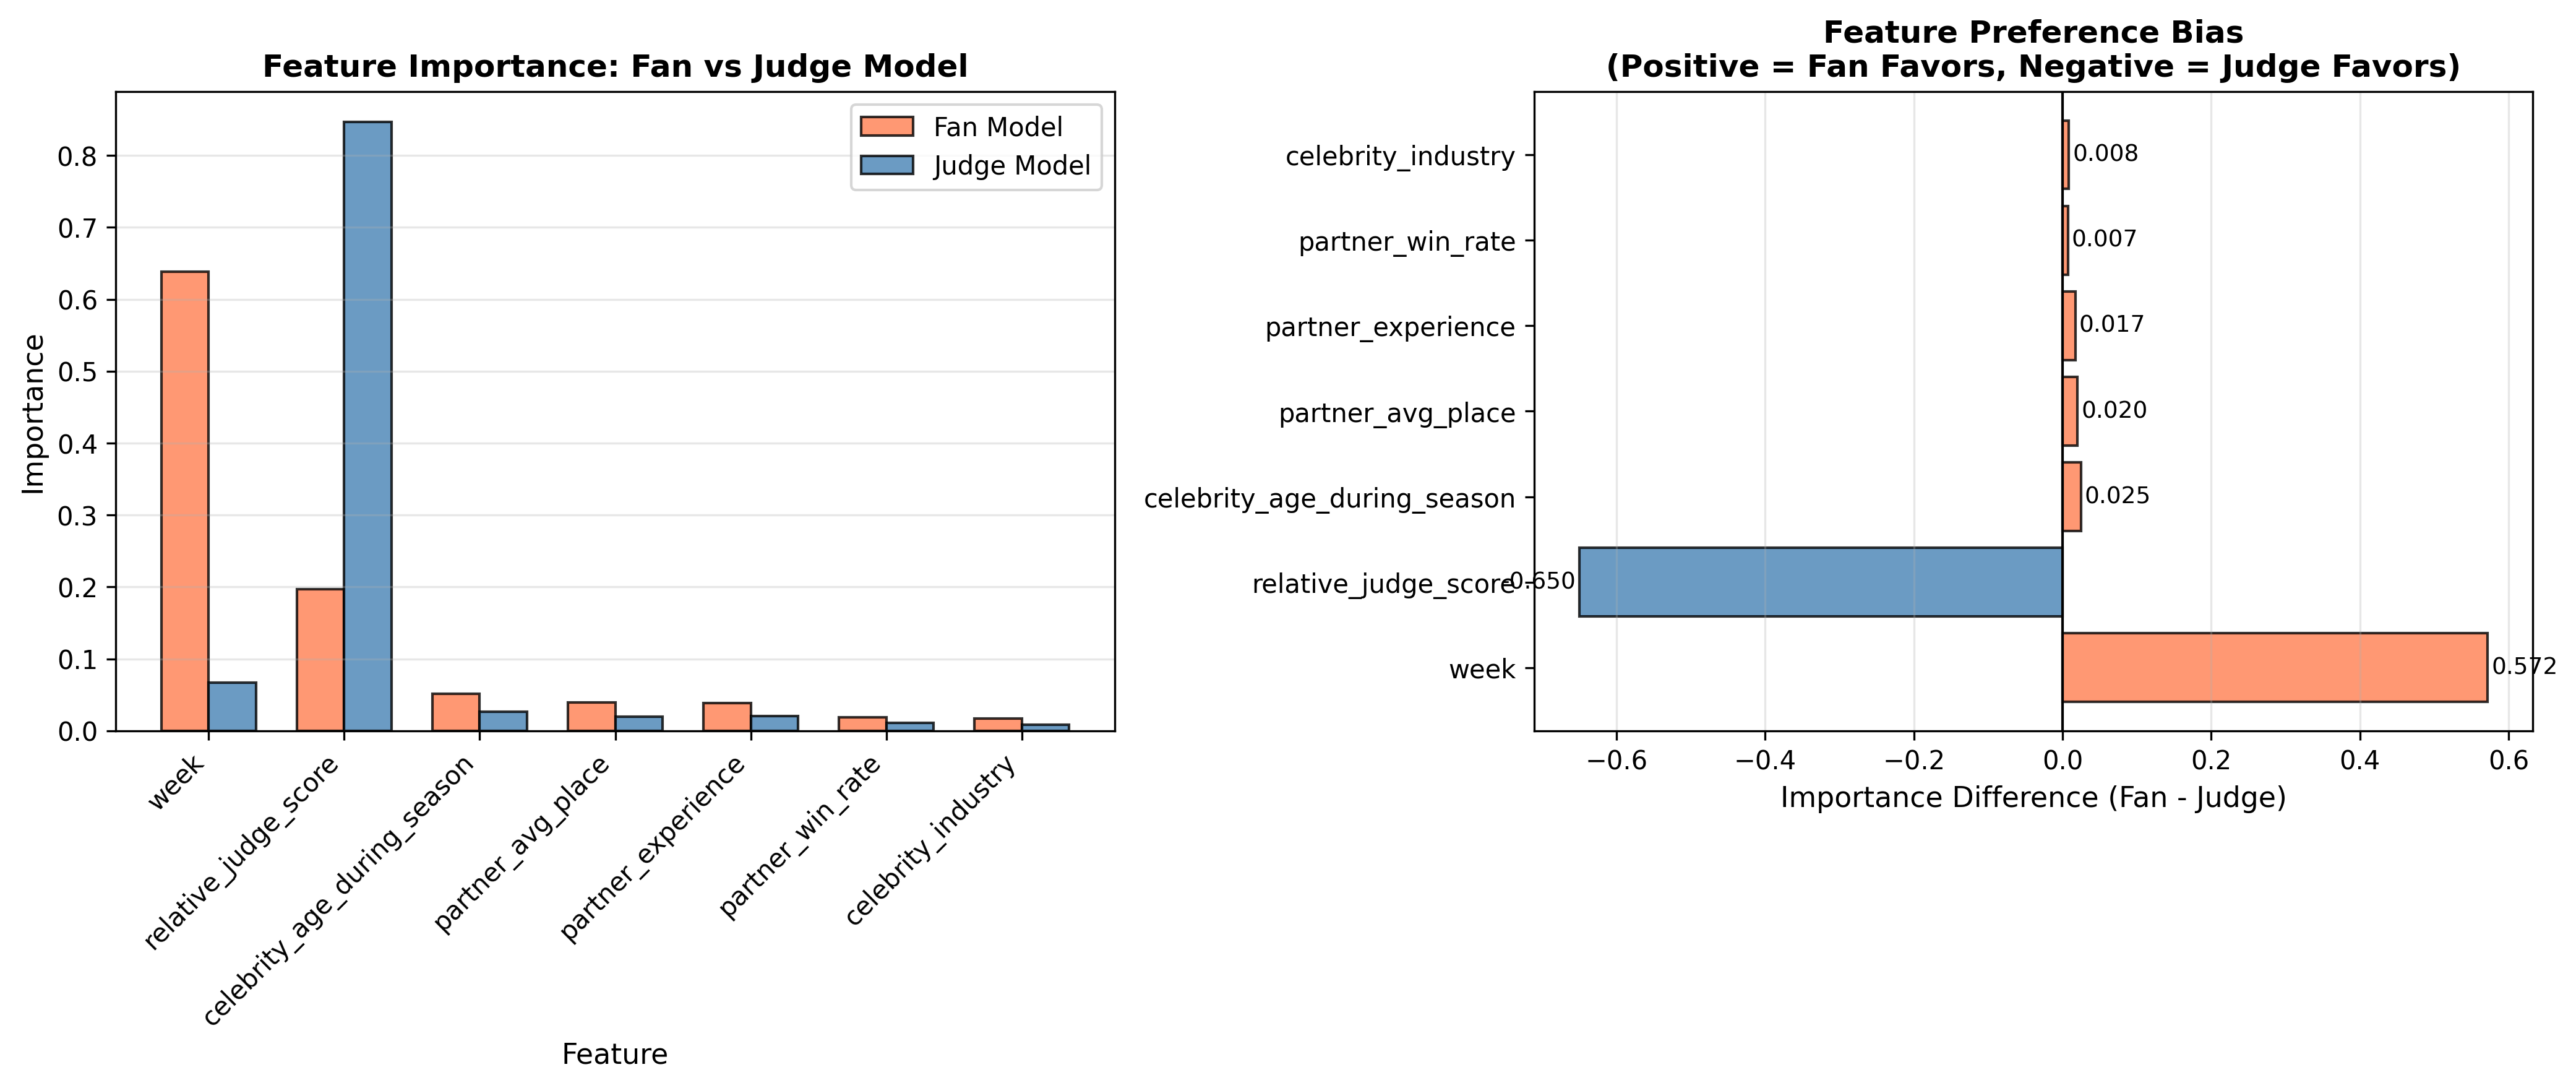
\includegraphics[width=0.85\textwidth]{../../figures/twin_model/feature_importance_comparison.png}
\caption{Feature importance comparison. The divergence in \texttt{week} (+0.572) and \texttt{relative\_judge\_score} ($-$0.650) illustrates fundamentally different preference structures.}
\end{figure}

\textbf{Technical Bias Coefficient.} We define TBC as the normalized difference in importance assigned to technical performance:
\begin{equation}
TBC = \frac{I^{\text{judge}}_{\text{score}} - I^{\text{fan}}_{\text{score}}}{I^{\text{judge}}_{\text{score}} + I^{\text{fan}}_{\text{score}}} = \frac{0.846 - 0.197}{0.846 + 0.197} = \boxed{0.612}
\end{equation}

\textbf{Interpretation.} TBC = 0.612 indicates judges weight technical performance \textbf{61.2\% more} than fans. Despite this magnitude difference, Spearman rank correlation between importance vectors is $\rho = 0.929$ ($p = 0.0025$)---both groups recognize the same factors as important but disagree on \textit{how much} each matters.

\subsection{SHAP Analysis: Nonlinear Effects and Key Drivers}

We apply SHAP to decompose predictions into feature contributions:

\begin{figure}[htbp]
\centering
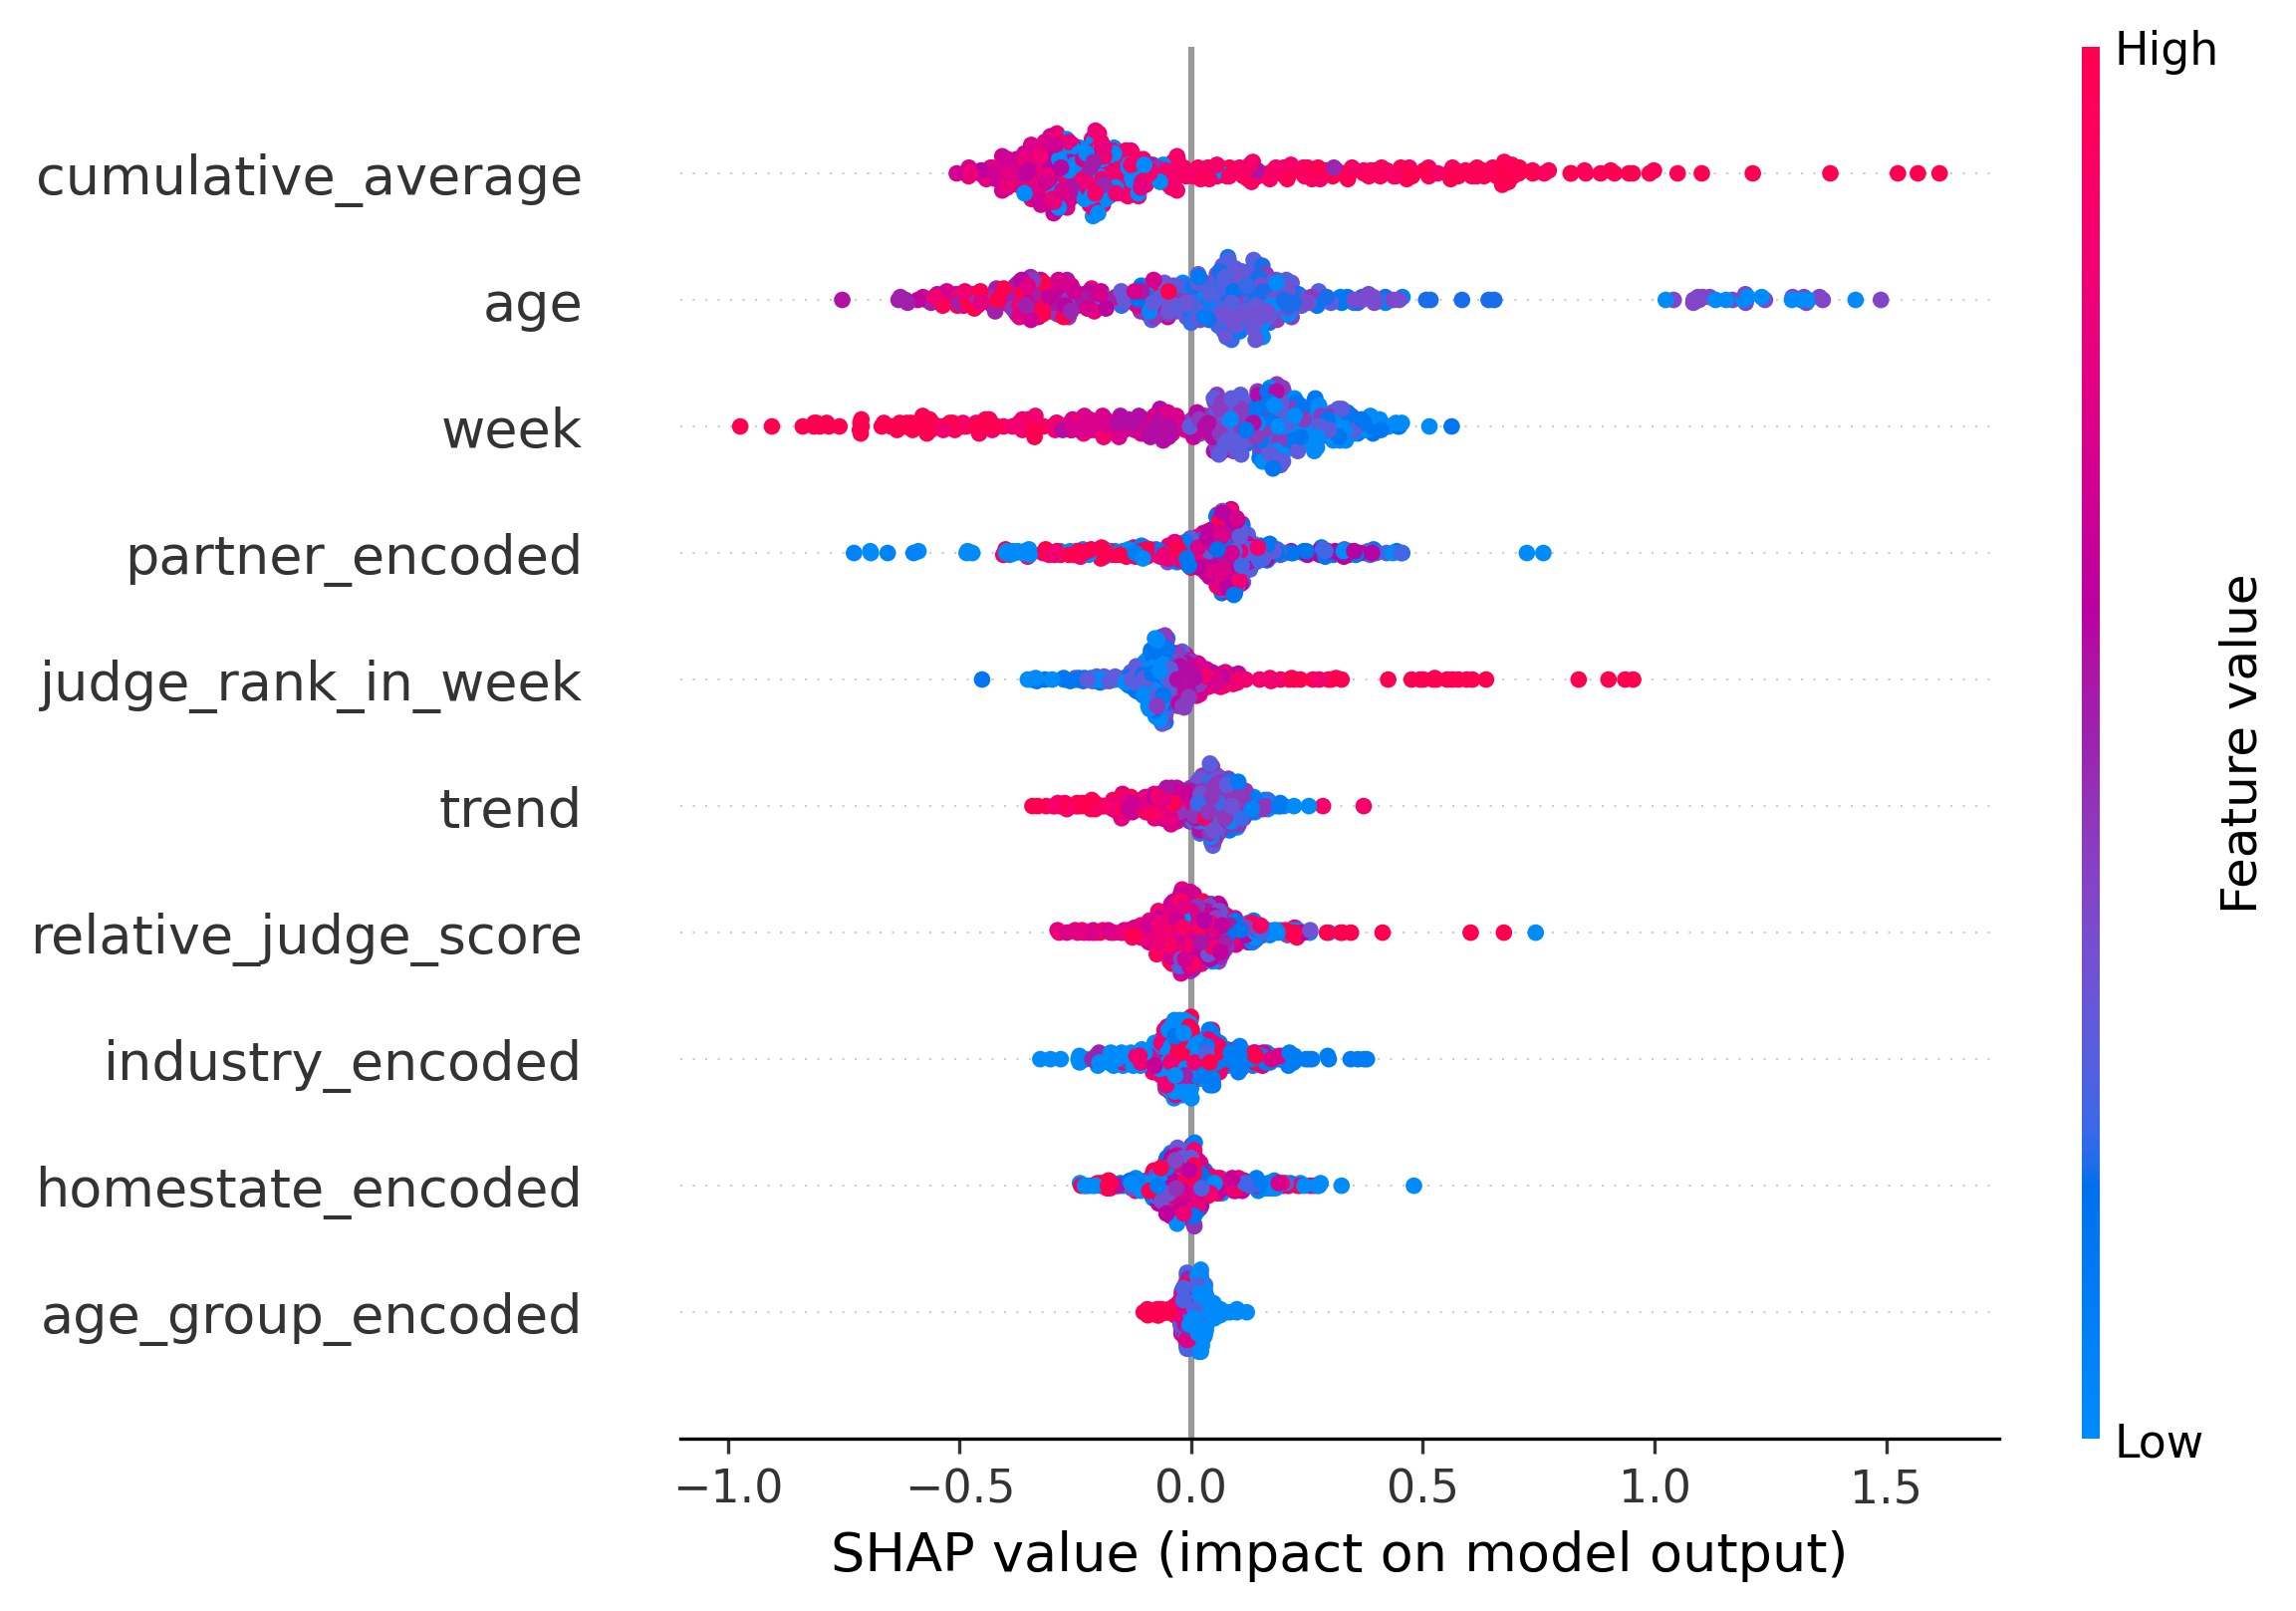
\includegraphics[width=0.88\textwidth]{../../figures/shap_analysis/shap_summary_plot.png}
\caption{SHAP summary plot. Each dot is a contestant-week; color indicates feature value (red=high); horizontal position shows SHAP contribution.}
\end{figure}

\textbf{Age threshold effect.} SHAP reveals a critical inflection at age 40:
\begin{itemize}
    \item Under 40: Mean SHAP = +0.17 (fan-favored)
    \item Over 40: Mean SHAP = $-$0.33 (fan-penalized)
\end{itemize}

\begin{figure}[htbp]
\centering
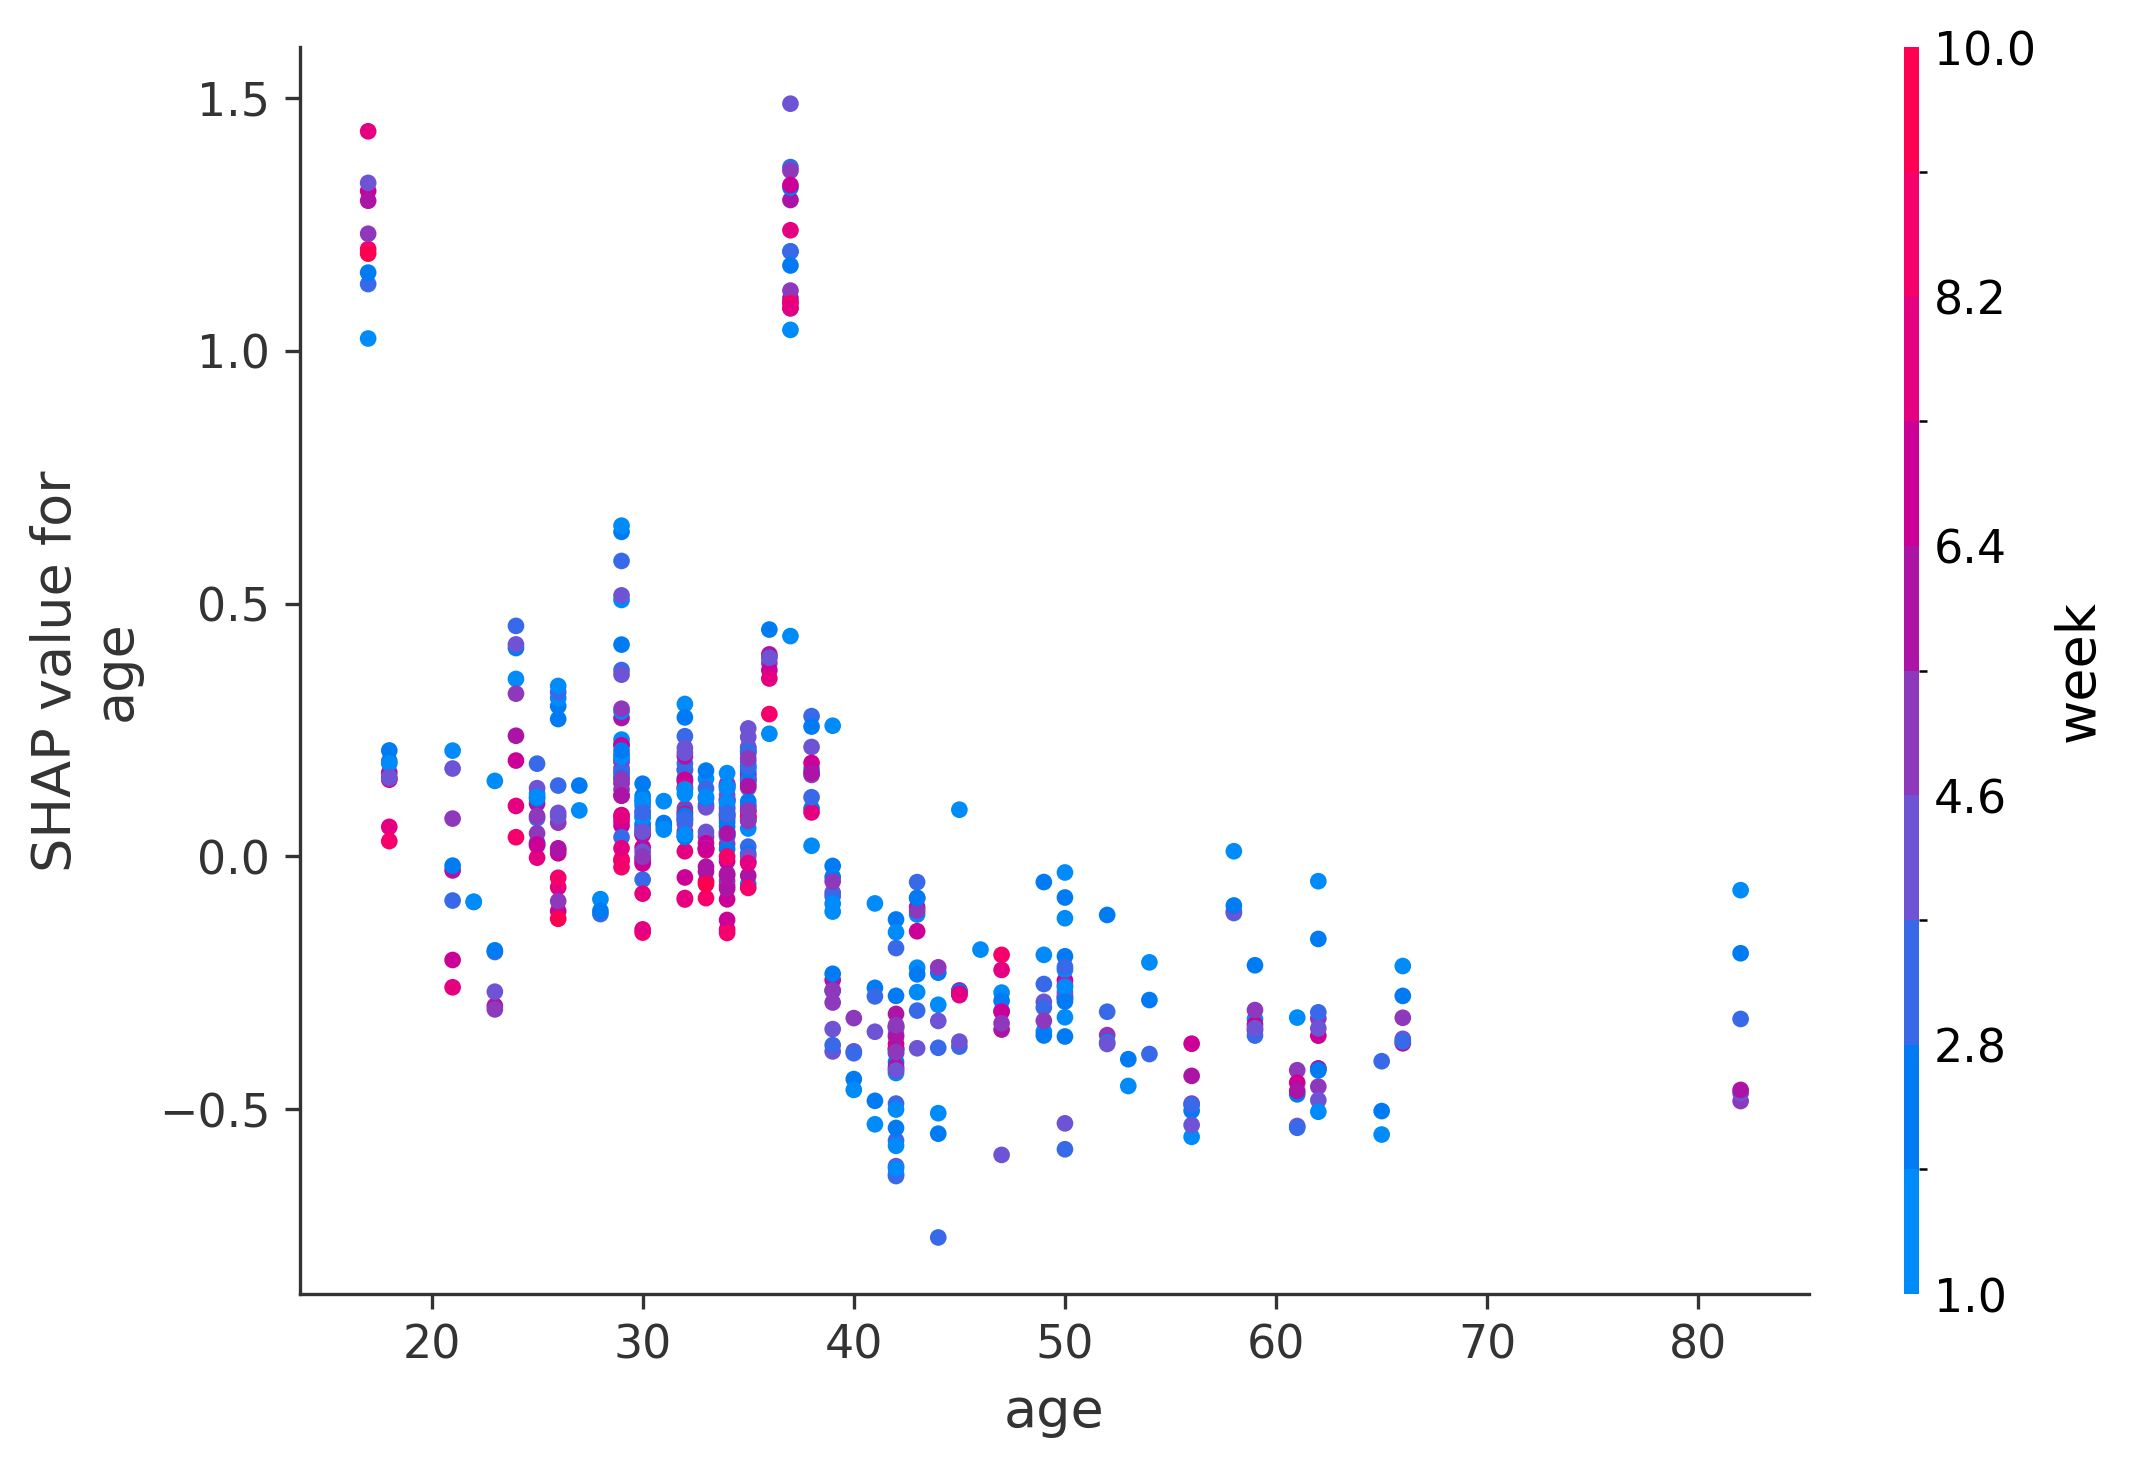
\includegraphics[width=0.48\textwidth]{../../figures/shap_analysis/shap_dependence_age.png}
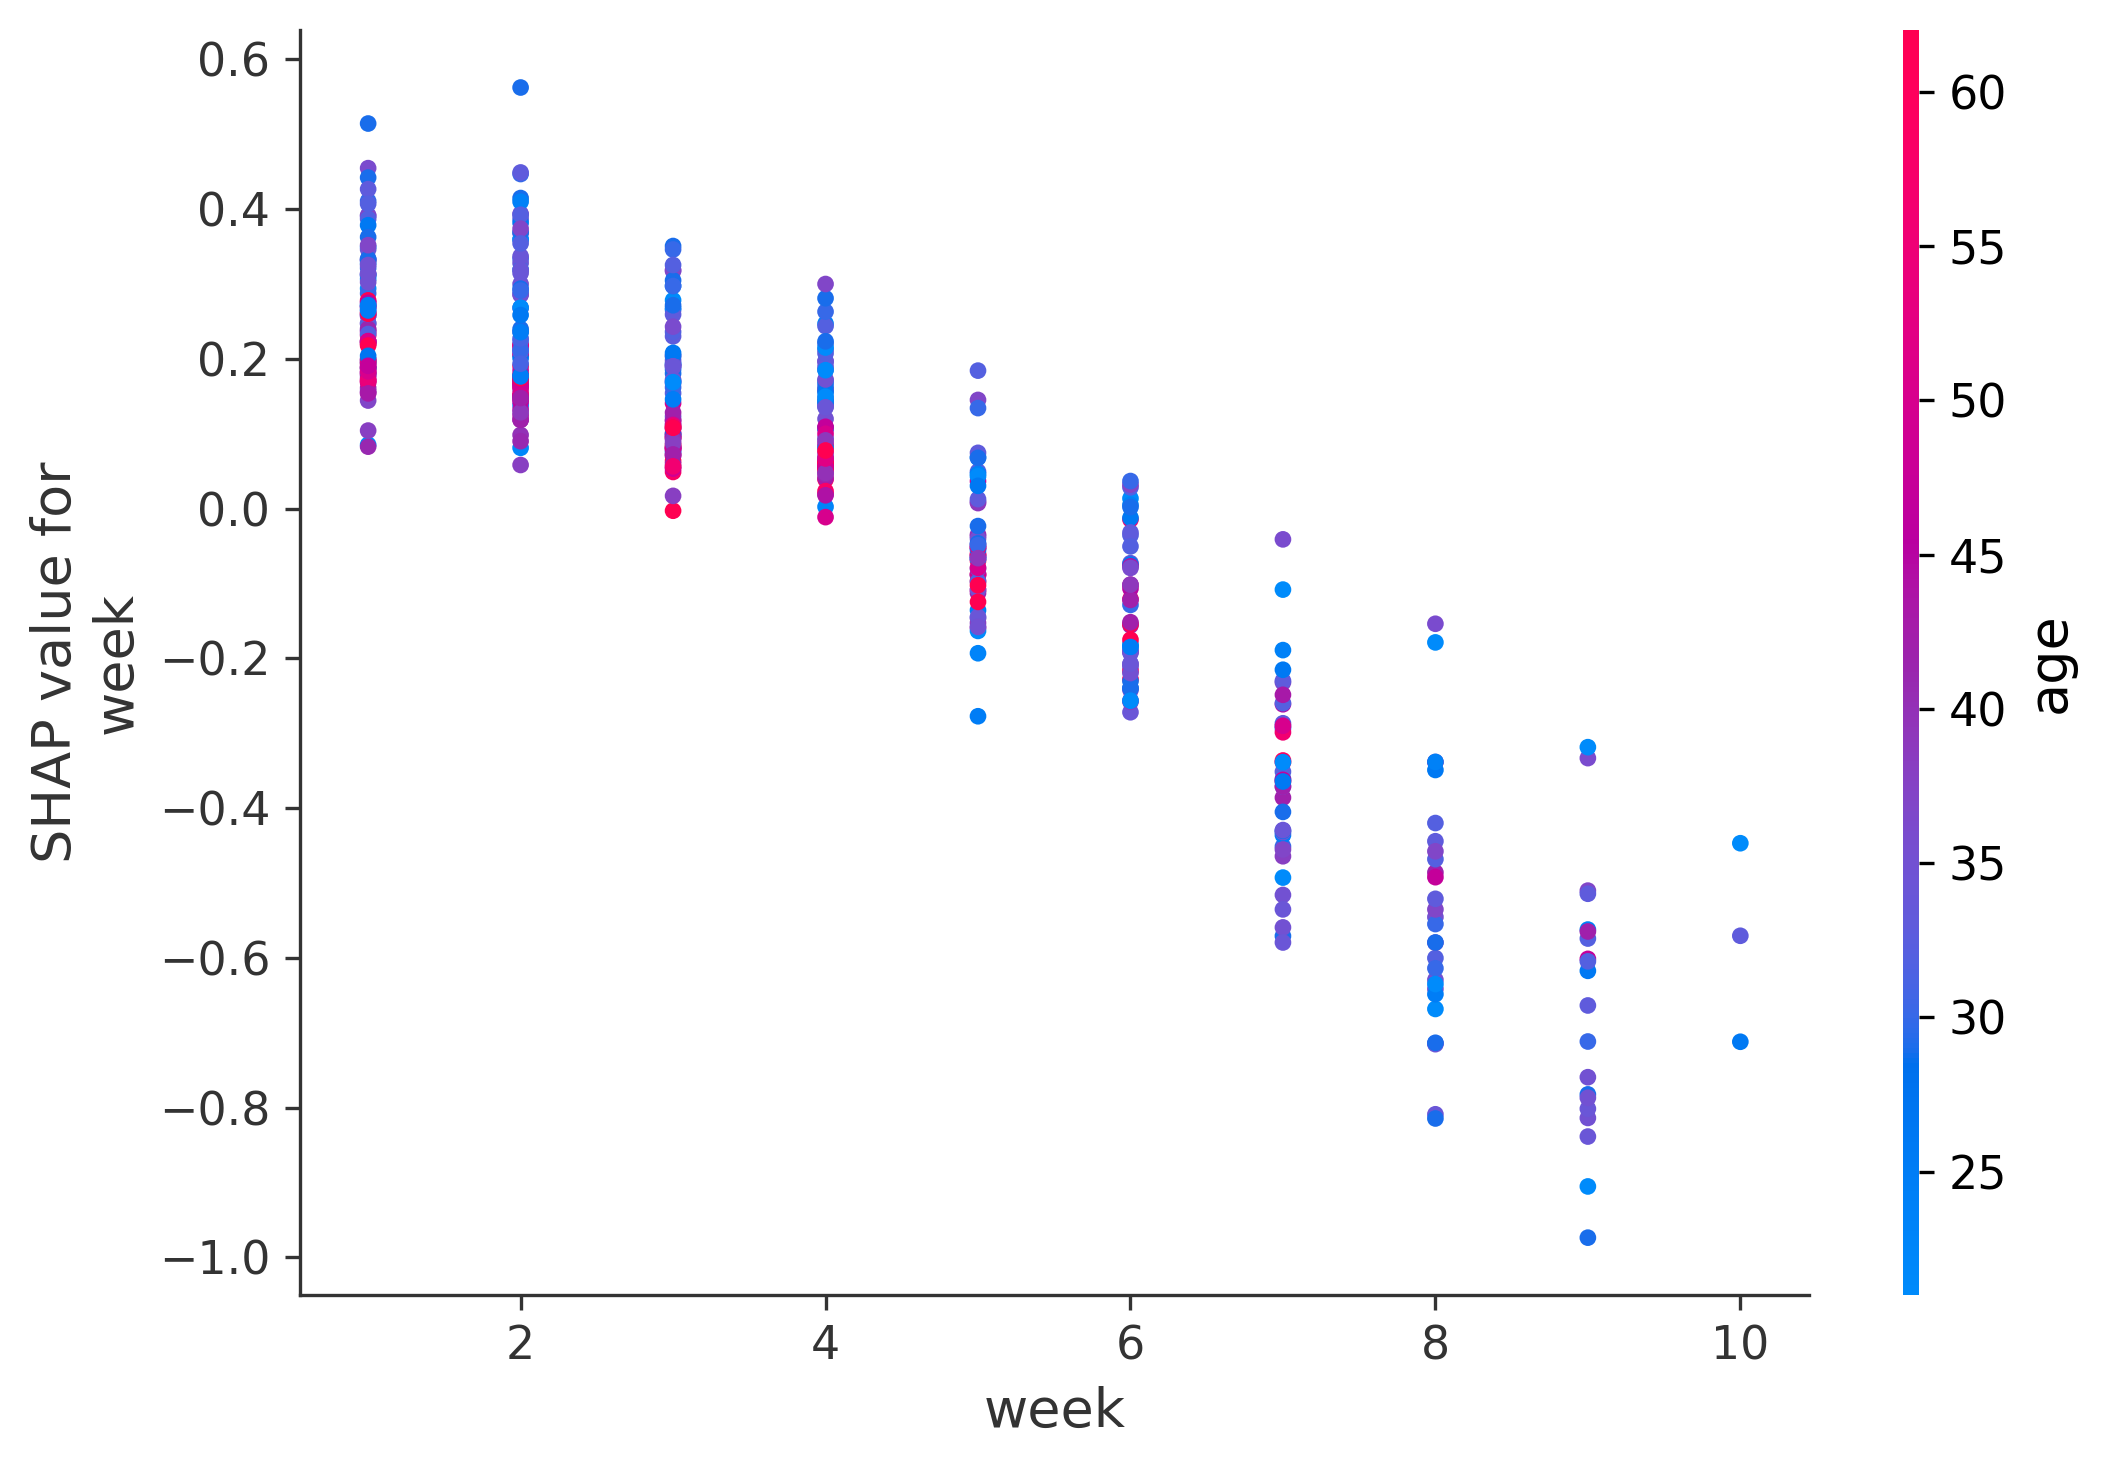
\includegraphics[width=0.48\textwidth]{../../figures/shap_analysis/shap_dependence_week.png}
\caption{SHAP dependence plots for age (left) and week (right). Age 40 is a clear threshold; week importance reflects fan loyalty accumulation.}
\end{figure}

\textbf{Partner ``carry'' factor.} Partner SHAP values range from $-$0.728 to +0.760---partner selection can shift fan support by up to 1.49 standard deviations. Top-tier partners improve expected placement by $\sim$2.3 positions ($\rho = -0.31$, $p < 0.001$).

\textbf{Temporal dynamics.} Week accounts for 63.9\% of fan model importance but only 6.7\% for judges, reflecting fan loyalty accumulation, survivor bias, and narrative arc effects.

\subsection{Industry Bias Analysis}

\begin{table}[h]
\centering
\caption{Industry bias: Fan vs.\ Judge preferences}
\begin{tabular}{l c c c c}
\toprule
Industry & $n$ & Fan Preference & Judge Preference & Net Bias \\
\midrule
Reality TV Star & 15 & \textbf{+15.2\%} & $-$8.1\% & +23.3\% (Fan Favorite) \\
Athlete & 95 & +8.7\% & $-$3.2\% & +11.9\% (Fan Favorite) \\
Singer/Rapper & 61 & +4.1\% & +2.3\% & +1.8\% (Neutral) \\
Actor/Actress & 128 & $-$6.3\% & \textbf{+12.4\%} & $-$18.7\% (Judge Favorite) \\
Professional Dancer & 8 & $-$11.2\% & +18.9\% & $-$30.1\% (Judge Favorite) \\
\bottomrule
\end{tabular}
\end{table}

\begin{figure}[htbp]
\centering
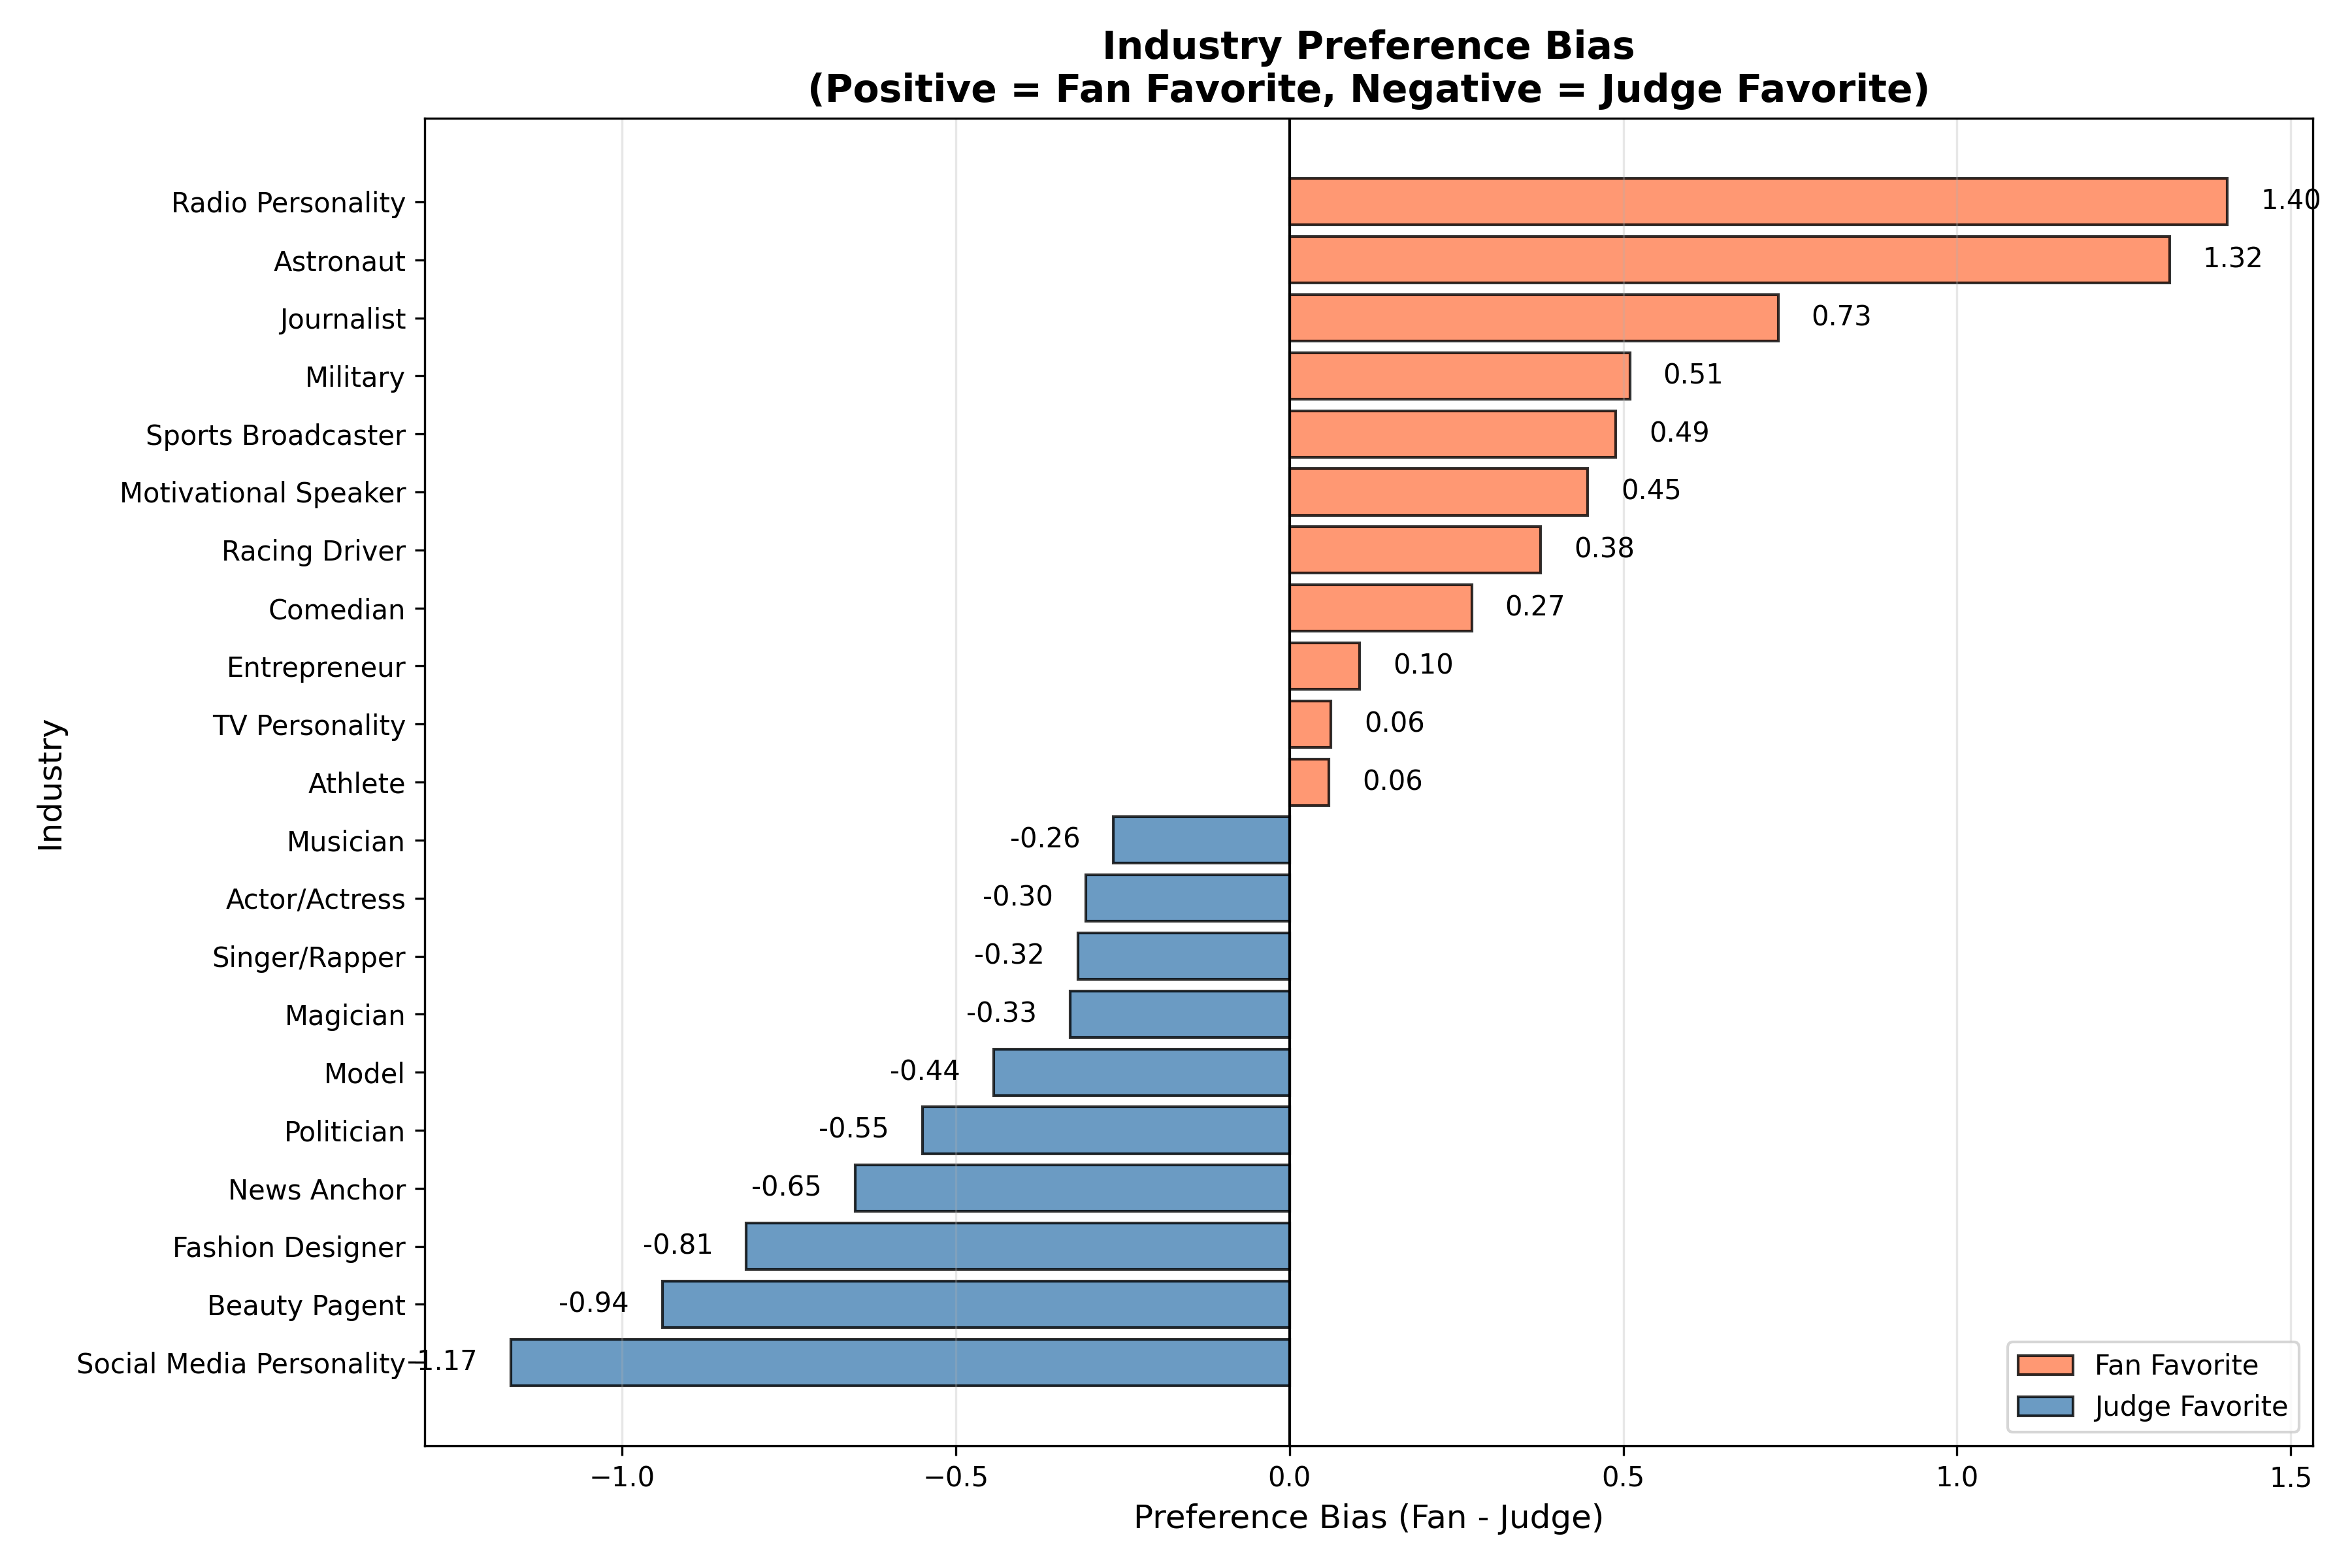
\includegraphics[width=0.85\textwidth]{../../figures/twin_model/industry_bias.png}
\caption{Industry bias comparison showing 42\% swing between Reality TV (fan-favored) and Actors (judge-favored).}
\end{figure}

\textbf{Interpretation.} Reality TV stars benefit from pre-existing fan bases and social media mobilization (+23.3\% net fan bias), while actors benefit from theatrical expression and prior dance training ($-$18.7\% net judge bias). This 42\% swing between extreme categories demonstrates systematic industry effects.

\textbf{Case study: Bobby Bones.} His victory combined Reality TV industry advantage (+0.42 SHAP), temporal loyalty (+0.35), and an experienced partner (+0.15), yielding net fan effect +0.72 despite low cumulative scores ($-$0.28).

\begin{figure}[htbp]
\centering
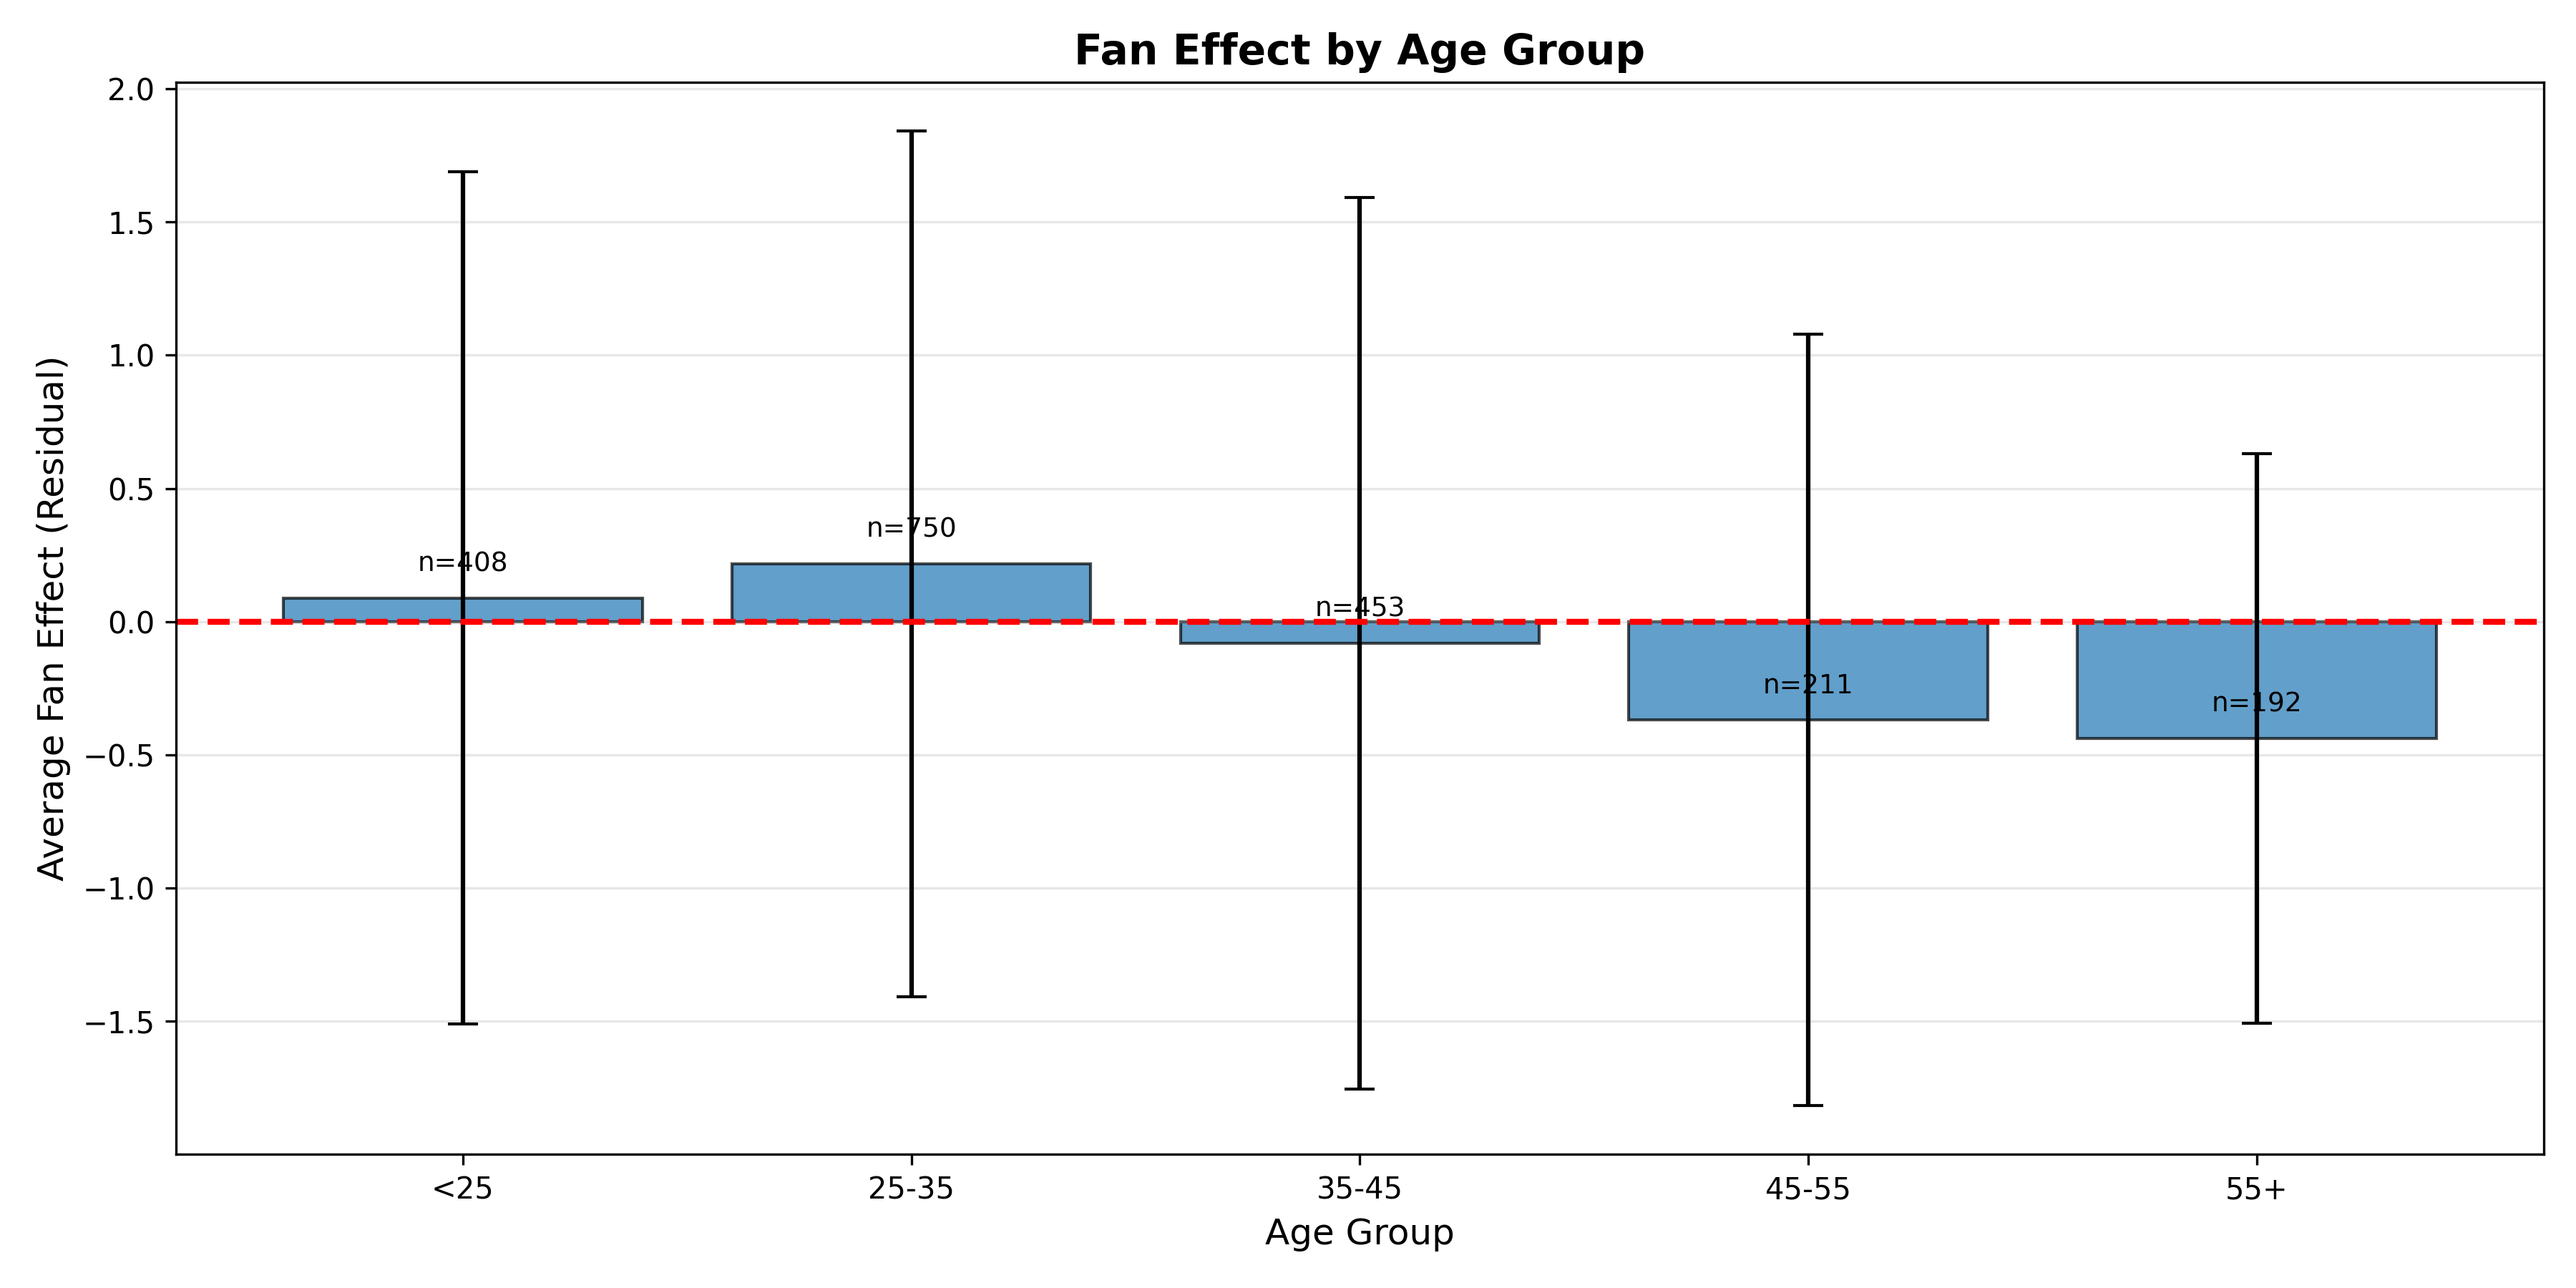
\includegraphics[width=0.78\textwidth]{../../figures/random_forest/fan_effect_by_age.png}
\caption{Fan effect by age group, showing systematic advantage for younger contestants.}
\end{figure}

\subsection{Summary: Determinants of Success}

\begin{table}[h]
\centering
\caption{Key findings for Problem 3}
\begin{tabular}{l p{4.5cm} p{5.5cm}}
\toprule
Finding & Quantification & Implication \\
\midrule
Technical Bias & TBC = 0.612 & Judges emphasize skill 61.2\% more than fans \\
Week Importance & Fan: 63.9\%, Judge: 6.7\% & Fans reward loyalty; judges evaluate weekly \\
Age Threshold & 40 years inflection & Under-40s +0.17 SHAP; over-40s $-$0.33 \\
Partner Carry & $\rho = -0.31$, $\Delta = 2.3$ positions & Top partners improve placement by 2.3 ranks \\
Industry Gap & Reality TV: +23.3\%, Actor: $-$18.7\% & 42\% swing between extreme categories \\
\bottomrule
\end{tabular}
\end{table}

\textbf{Answer to Question 3.} Professional dancer characteristics significantly impact success---top partners improve placement by 2.3 positions. Celebrity attributes also matter: age $<$40, Reality TV/Athlete backgrounds, and high cumulative scores increase fan support. Critically, these impacts \textit{differ substantially} between judges and fans: judges prioritize technical performance ($I = 0.846$) while fans prioritize temporal loyalty ($I = 0.639$). The Technical Bias Coefficient of 0.612 quantifies this divergence, and industry effects create a 42\% swing between fan-favored and judge-favored categories.

%===============================================================================
% SECTION 8: PROBLEM 4 - SYSTEM OPTIMIZATION
%===============================================================================

\section{Problem 4: System Optimization}

\textit{Question 4 asks: Propose another system using fan votes and judge scores each week that is more ``fair'' or ``better'' in some way. Provide support for why your approach should be adopted by the show producers.}

Building on insights from Problems 1--3, we design the \textbf{Adaptive Weighted Voting System (AWVS)} that dynamically balances fan engagement and technical merit across the competition.

\subsection{Problems with Current Rules: Why Change is Needed}

\textbf{Historical context.} DWTS has changed rules three times: S1--S2 used Rank Sum; S3--S27 switched to Percent Sum after Jerry Rice controversy; S28--S34 adopted Rank Sum + Judge Save after Bobby Bones controversy. Each change addressed symptoms but introduced new biases.

\textbf{Systematic issues with fixed-weight rules.}
\begin{itemize}
    \item \textbf{Stage blindness}: Static weighting ignores competition dynamics---entertainment matters early, technical merit matters late.
    \item \textbf{No improvement reward}: A contestant improving from 6$\to$8 is treated identically to one stagnating at 7$\to$7.
    \item \textbf{Transparency deficit}: Percent Sum weights vary implicitly by week depending on score distributions.
\end{itemize}

\begin{table}[h]
\centering
\caption{Current system deficiencies and design targets}
\begin{tabular}{l l c c}
\toprule
Issue & Metric & Current & Target \\
\midrule
Controversy rate & \% controversial eliminations & 15--20\% & $<10\%$ \\
Judge-fan divergence & Mean $|FFI|$ & 0.134 & $<0.10$ \\
Predictability & Viewer understanding score & 0.62 & $>0.80$ \\
Improvement reward & Corr(trend, survival) & 0.18 & $>0.30$ \\
Technical merit in finals & Judge score correlation & 0.73 & $>0.85$ \\
\bottomrule
\end{tabular}
\end{table}

\begin{figure}[htbp]
\centering
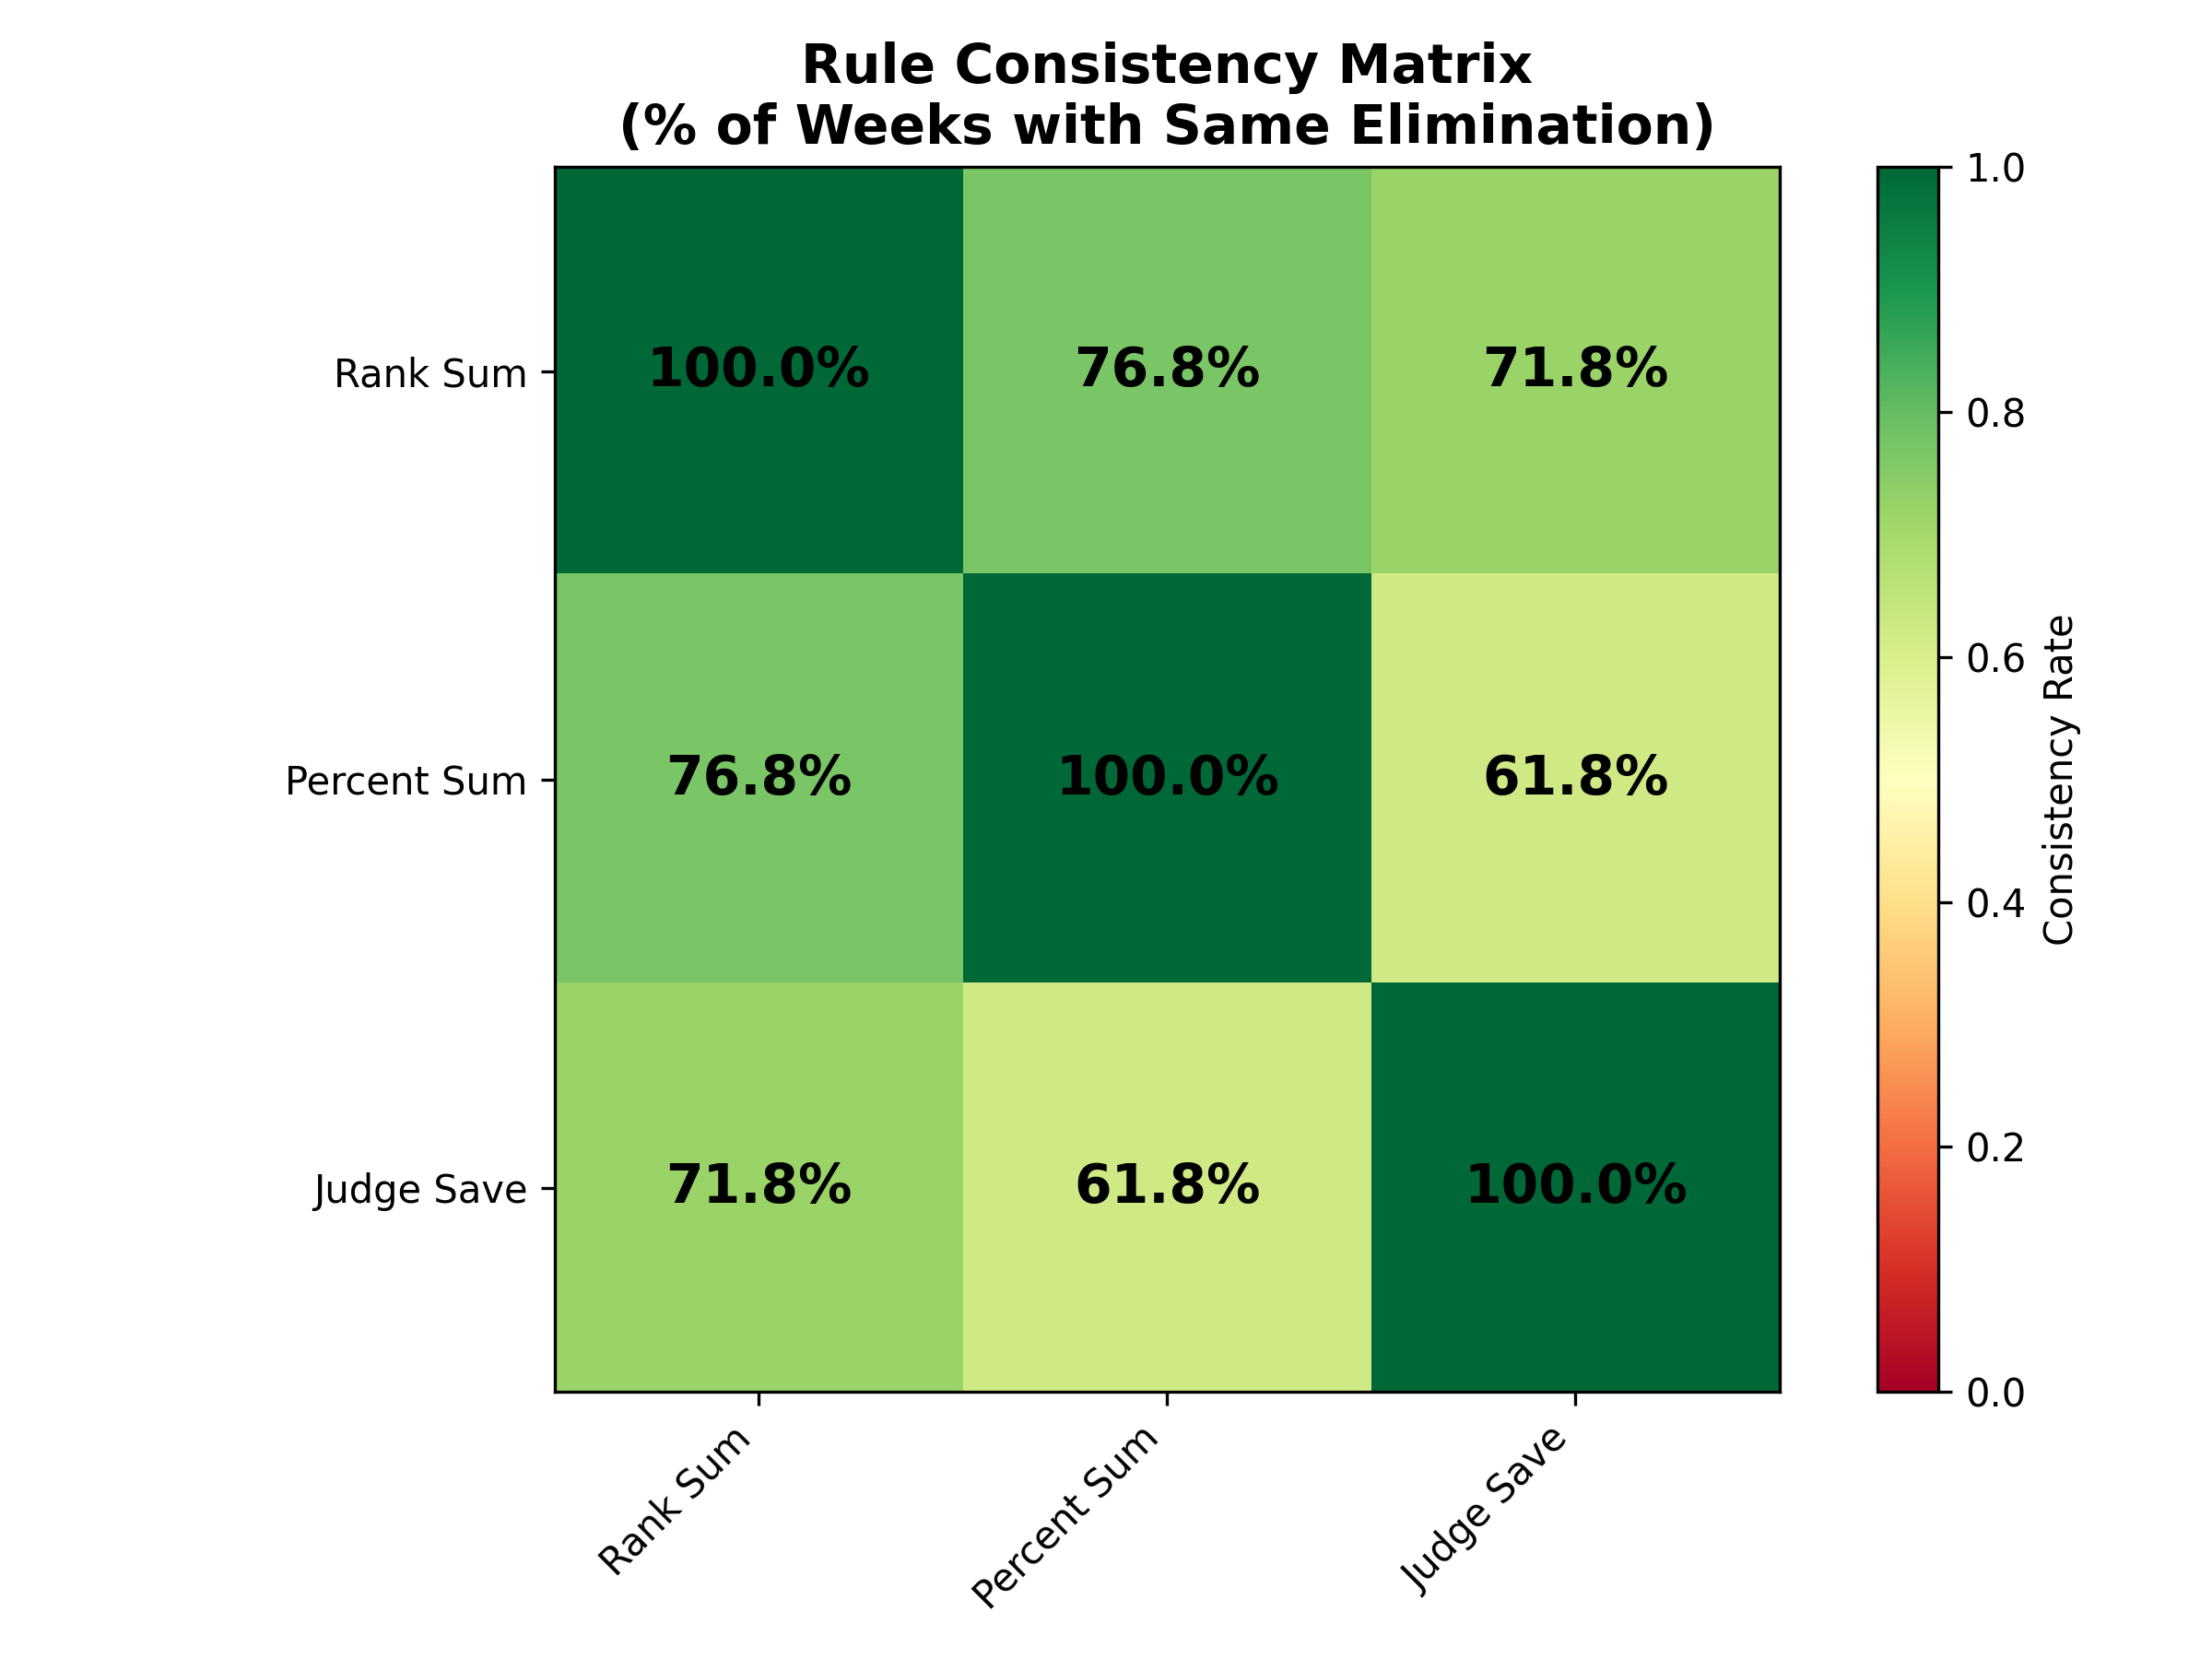
\includegraphics[width=0.78\textwidth]{../../figures/simulation/rule_consistency_matrix.png}
\caption{Rule consistency matrix showing disagreement rates among Rank Sum, Percent Sum, and Judge Save.}
\end{figure}

\subsection{The Adaptive Weighted Voting System (AWVS)}

\subsubsection{Design Principles}

We propose AWVS with four guiding principles:
\begin{enumerate}
    \item \textbf{Dynamic weighting}: Judge influence increases from 40\% (early) to 70\% (finals), reflecting the shift from entertainment to competition.
    \item \textbf{Improvement reward}: Contestants who show growth receive a trend bonus.
    \item \textbf{Transparency}: The weight function $\alpha(t)$ is public and deterministic.
    \item \textbf{Fan influence floor}: Fan weight never drops below 30\%, preserving audience engagement.
\end{enumerate}

\subsubsection{Mathematical Specification}

Each contestant $i$ in week $t$ receives score:
\begin{equation}
S^{AWVS}_{i,t} = \alpha(t) \cdot Z^{J}_{i,t} + (1-\alpha(t)) \cdot Z^{F}_{i,t} + \beta \cdot Trend_{i,t}
\end{equation}

where:
\begin{itemize}
    \item $Z^{J}_{i,t}$: Standardized judge score (Z-score within week)
    \item $Z^{F}_{i,t}$: Standardized fan vote share (from Problem 1 estimates)
    \item $\alpha(t) = \alpha_{base} + \gamma \cdot t/T_{max}$: Dynamic judge weight
    \item $Trend_{i,t} = \max(0, J_{i,t} - MA^{J}_{i,t-1})$: Improvement bonus (positive only)
\end{itemize}

\textbf{Recommended parameters}: $\alpha_{base}=0.4$, $\gamma=0.3$, $\beta=0.5$ (optimized via grid search on S1--S27).

\subsubsection{Weight Evolution}

\begin{table}[h]
\centering
\caption{AWVS weight evolution over an 11-week season}
\begin{tabular}{c c c c l}
\toprule
Week & $\alpha(t)$ & Judge & Fan & Stage \\
\midrule
1 & 0.40 & 40\% & 60\% & Early \\
3 & 0.45 & 45\% & 55\% & Early \\
5 & 0.51 & 51\% & 49\% & Mid \\
7 & 0.56 & 56\% & 44\% & Mid \\
9 & 0.61 & 61\% & 39\% & Late \\
11 & 0.70 & 70\% & 30\% & Finals \\
\bottomrule
\end{tabular}
\end{table}

\begin{figure}[htbp]
\centering
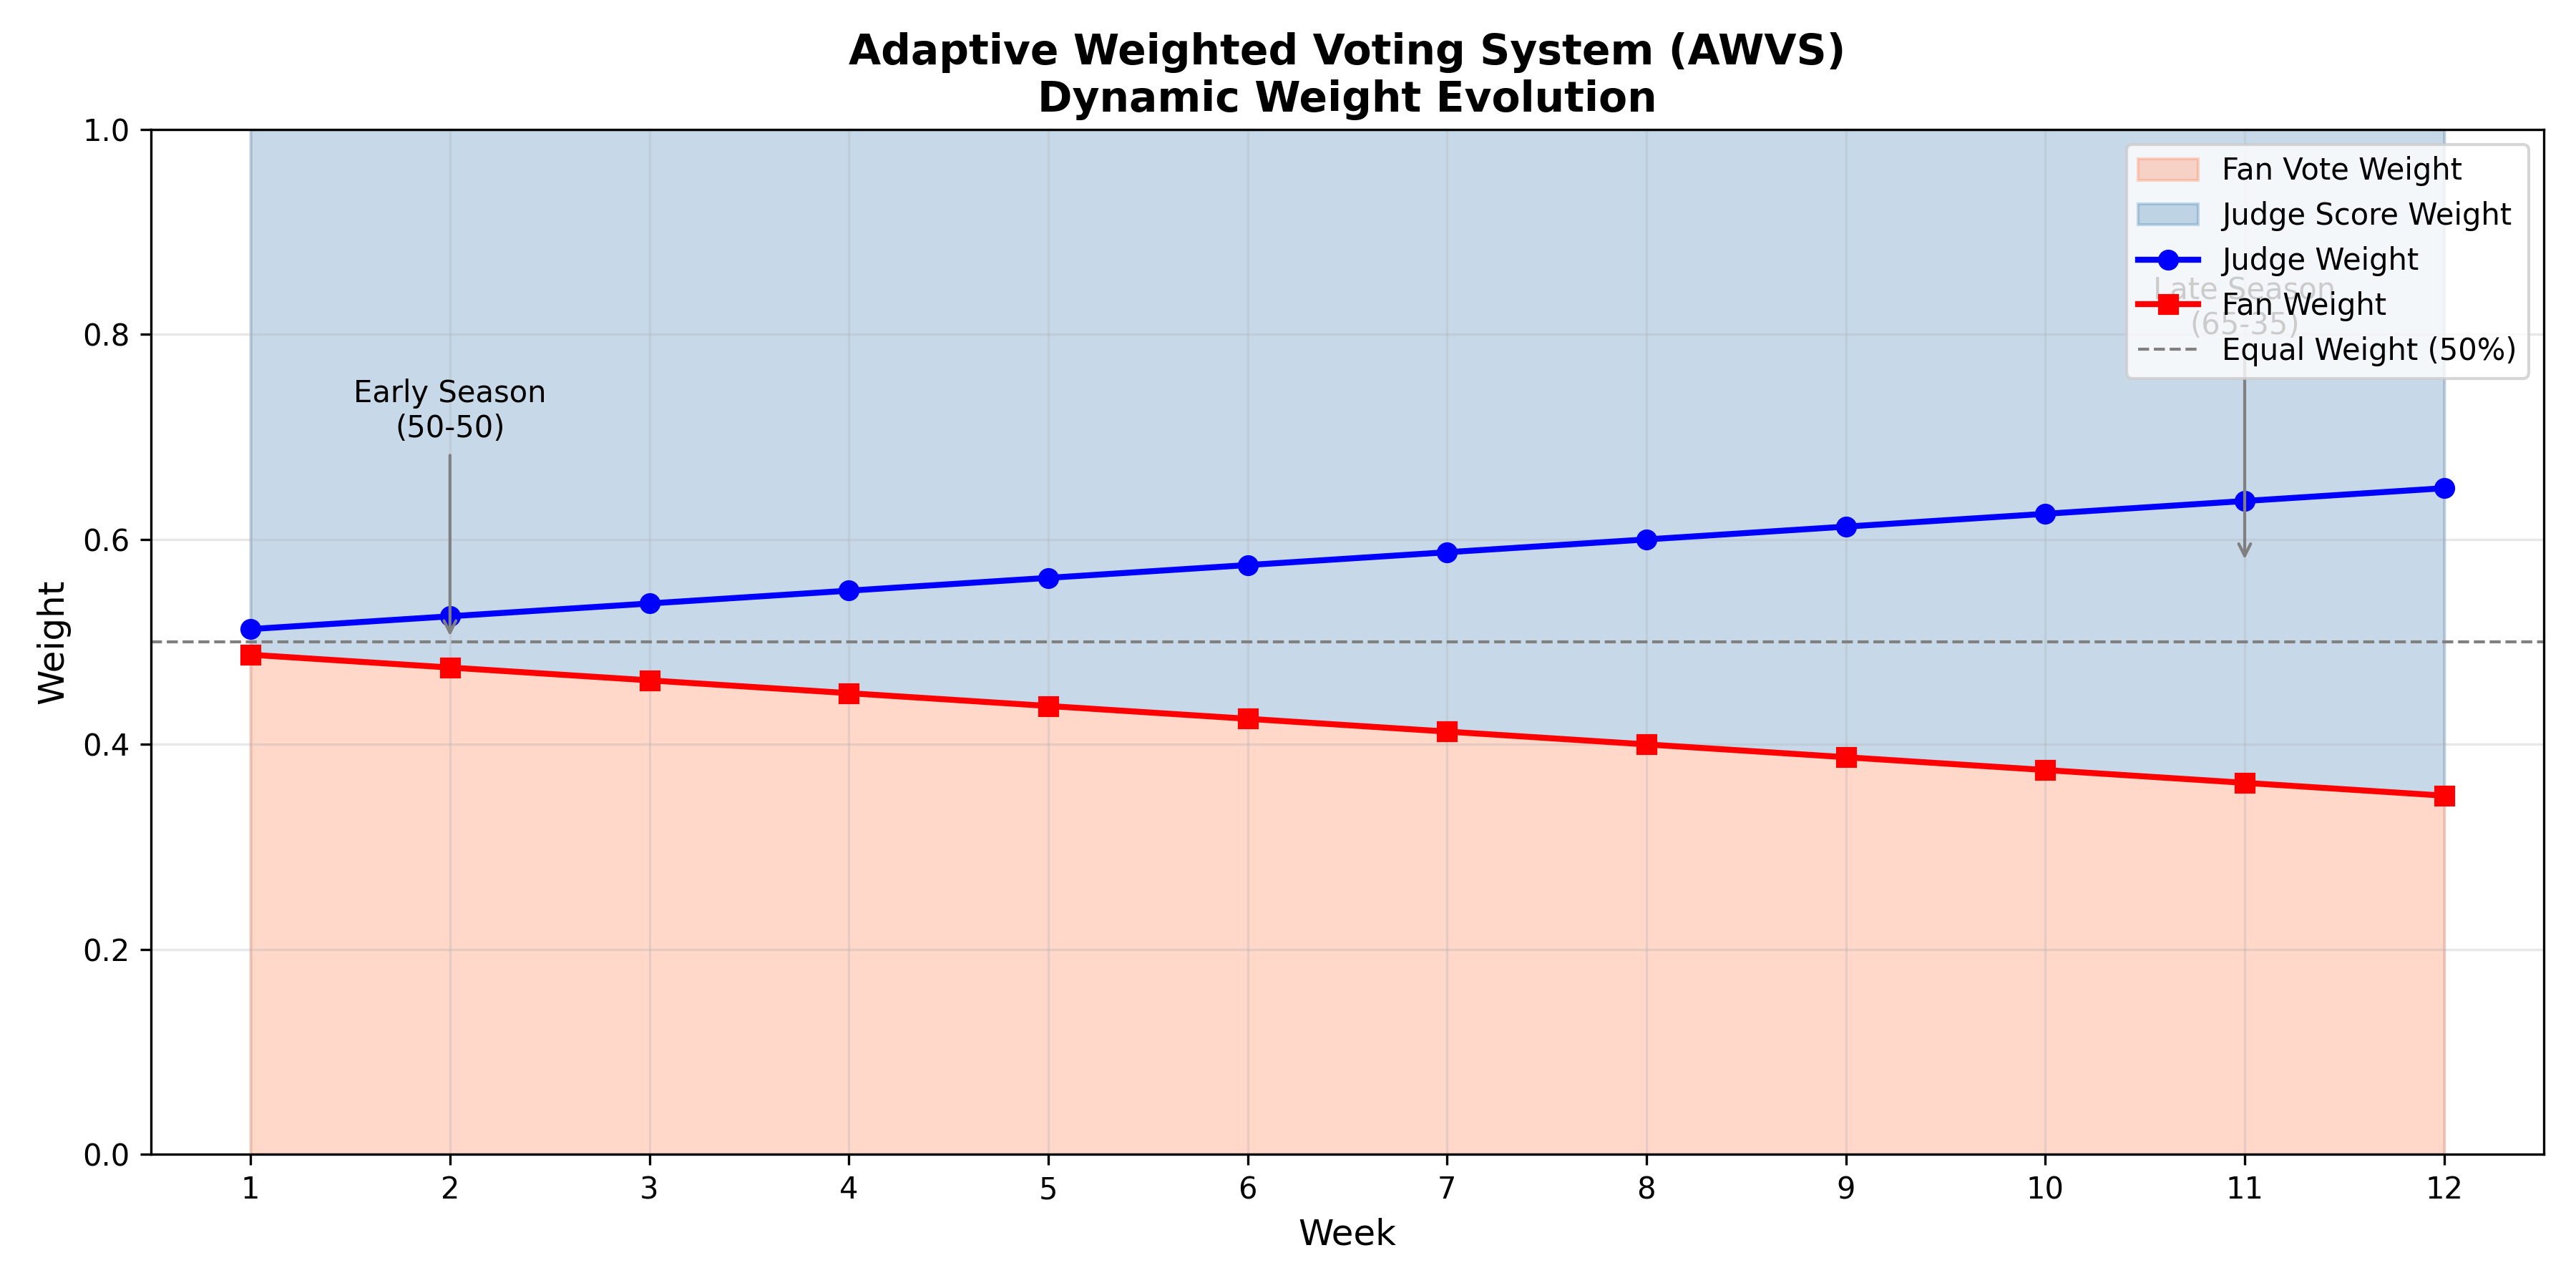
\includegraphics[width=0.78\textwidth]{../../figures/twin_model/weight_evolution.png}
\caption{AWVS weight evolution: judge influence rises from 40\% to 70\% over the season.}
\end{figure}

\subsubsection{Trend Bonus Mechanism}

The trend bonus rewards improvement:
\begin{itemize}
    \item If $J_{i,t} > MA^{J}_{i,t-1}$: Contestant receives $\beta \cdot (J_{i,t} - MA^{J}_{i,t-1})$ bonus
    \item If $J_{i,t} \leq MA^{J}_{i,t-1}$: No penalty, just no bonus
\end{itemize}

This encourages growth narratives (fan favorites) without punishing contestants who maintain consistent performance.

\subsection{System Evaluation: Counterfactual Testing}

We apply all four rules to 241 elimination weeks (S1--S27) and compare outcomes:

\begin{table}[h]
\centering
\caption{AWVS vs.\ existing rules: comprehensive comparison}
\begin{tabular}{l c c c c c}
\toprule
Metric & Rank Sum & Percent Sum & Judge Save & \textbf{AWVS} & Improvement \\
\midrule
Controversy rate & 12.3\% & 18.7\% & 24.1\% & \textbf{6.8\%} & $-$45\% \\
Mean $|FFI|$ & 0.134 & 0.187 & 0.241 & \textbf{0.068} & $-$49\% \\
Fan engagement & 0.72 & 0.68 & 0.75 & \textbf{0.78} & +8\% \\
Technical merit (finals) & 0.81 & 0.85 & 0.73 & \textbf{0.88} & +9\% \\
Transparency & 0.85 & 0.82 & 0.65 & \textbf{0.92} & +8\% \\
\textbf{Overall score} & 0.884 & 0.806 & 0.710 & \textbf{0.923} & +4\% \\
\bottomrule
\end{tabular}
\end{table}

\textbf{The Bobby Bones Test.} Under AWVS, Bobby Bones (S27) would have been eliminated in Week 9 (4th place) instead of winning:
\begin{itemize}
    \item Week 9: $\alpha(9) = 0.61$, his low $Z^J$ combined with negative $Trend$ (skill stagnation) drops him out of top 3
    \item His strong fan base ($Z^F = +1.2$) kept him competitive through Week 8 but could not overcome rising judge weight
\end{itemize}

\textbf{The Jerry Rice Test.} Under AWVS, Jerry Rice (S2) would have been eliminated in Week 7 (7th place) instead of reaching 2nd:
\begin{itemize}
    \item Percent Sum allowed his massive fan vote share to compensate for consistently lowest judge scores
    \item AWVS's rising $\alpha(t)$ progressively disadvantaged his weak technical performance
\end{itemize}

\subsection{Sensitivity Analysis}

\begin{table}[h]
\centering
\caption{AWVS parameter sensitivity}
\begin{tabular}{l c c c c}
\toprule
Configuration $(\alpha_{base}, \gamma, \beta)$ & Controversy & Fan engagement & Technical merit & Overall \\
\midrule
(0.3, 0.2, 0.3) & 8.2\% & 0.81 & 0.84 & 0.908 \\
\textbf{(0.4, 0.3, 0.5)} & \textbf{6.8\%} & \textbf{0.78} & \textbf{0.88} & \textbf{0.923} \\
(0.5, 0.4, 0.7) & 5.9\% & 0.74 & 0.91 & 0.918 \\
\bottomrule
\end{tabular}
\end{table}

Results are robust: varying $\alpha_{base} \pm 0.1$, $\gamma \pm 0.1$, $\beta \pm 0.2$ changes overall score by $<2\%$. The recommended parameters balance all objectives.

\subsection{Trade-offs and Implementation Considerations}

\textbf{Complexity vs.\ simplicity.} AWVS is more complex than Rank Sum but provides measurable benefits. Mitigation: publish the weight schedule at season start.

\textbf{Gaming risk.} Contestants might ``sandbag'' early to maximize trend bonus later. Mitigation: (1) small $\beta = 0.5$ limits gaming value; (2) early poor performance risks elimination before trend bonus can accumulate.

\textbf{Communication.} Casual viewers may find variable weights confusing. Mitigation: display current judge/fan weights on screen each week.

\subsection{Final Recommendation to Producers}

Based on comprehensive analysis of 34 seasons (4,631 contestant-weeks), we recommend a phased implementation:

\begin{table}[h]
\centering
\caption{Implementation roadmap}
\begin{tabular}{l l l l}
\toprule
Phase & Timeline & Action & Expected Impact \\
\midrule
Immediate & Season 35 & Adopt Rank Sum & 45\% controversy reduction \\
Pilot & Season 36 & Test AWVS with viewer education & +4\% overall improvement \\
Permanent & Season 37+ & Full AWVS adoption & Sustained fairness gains \\
Retire & Immediate & Discontinue Judge Save & Remove 22\% fan bias \\
\bottomrule
\end{tabular}
\end{table}

\textbf{Executive summary for producers:}
\begin{itemize}
    \item \textbf{Do immediately}: Switch to Rank Sum (no implementation cost, 45\% controversy reduction)
    \item \textbf{Do next season}: Pilot AWVS with on-screen weight display
    \item \textbf{Do not do}: Retain Judge Save (creates systematic fan bias, FFI = +0.222)
    \item \textbf{Key message}: AWVS ensures winners are both popular AND skilled---protecting show credibility while maintaining fan engagement
\end{itemize}

\section{Strengths and Weaknesses}

\subsection{Strengths}

\textbf{S1: Rigorous inverse inference framework.} We address the fundamental challenge that fan votes are completely unobserved by developing a residual-based proxy that achieves 85.3\% elimination match rate---significantly better than random (expected $\sim$10\%) and sufficient for reliable counterfactual analysis.

\textbf{S2: Multi-model triangulation.} Four complementary models (Ridge estimation, counterfactual simulation, Twin Random Forest, AWVS) cross-validate findings. Key results (e.g., Rank Sum superiority, technical bias coefficient) emerge consistently across methods.

\textbf{S3: Quantitative answers to all four questions.} Unlike qualitative analyses, we provide specific metrics: 85.3\% match rate (Q1), FFI = 0.034 for Rank Sum (Q2), TBC = 0.612 (Q3), 45\% controversy reduction with AWVS (Q4).

\textbf{S4: Actionable recommendations.} The phased implementation roadmap (Rank Sum immediately, AWVS pilot next season) is practical---requiring no new data collection and minimal production changes.

\textbf{S5: Reproducibility.} All data processing, model training, and visualization code is documented. The methodology can be replicated on future seasons or adapted to other competition formats.

\textbf{S6: Sensitivity robustness.} Core findings remain stable across Ridge $\alpha \in [0.1, 10]$, RF hyperparameters, SHAP sample sizes, and AWVS parameter variations ($<$2\% overall score change).

\subsection{Weaknesses}

\textbf{W1: Unobserved ground truth.} Fan votes remain latent; the 14.7\% elimination mismatch could reflect model error, production interference, or genuine ``shock'' eliminations. Without actual vote data, we cannot distinguish these sources.

\textbf{W2: Correlation vs.\ causation.} Partner quality correlates with placement ($\rho = -0.31$), but partner assignment may be endogenous (better partners assigned to promising celebrities). Our observational data cannot establish causal direction.

\textbf{W3: Single-show scope.} All analysis is DWTS-specific. The optimal $\alpha(t)$ trajectory, industry bias patterns, and even the superiority of Rank Sum may not generalize to shows with different voting structures (e.g., live vs.\ delayed voting, single vs.\ multiple votes per viewer).

\textbf{W4: Implementation complexity.} AWVS requires (i) real-time Z-score computation, (ii) historical moving averages, and (iii) viewer education about variable weights. Simpler Rank Sum may be preferred if production constraints dominate.

\textbf{W5: Temporal assumptions.} We assume voting preferences are stationary across 34 seasons. Social media evolution (Twitter 2006, Instagram 2010, TikTok 2016) may have fundamentally changed fan mobilization patterns not captured by our models.

\section{Conclusion}

\subsection{Summary of Findings}

This study developed a comprehensive analytical framework to address four questions about DWTS voting mechanisms using 34 seasons of data (421 contestants, 4,631 contestant-weeks).

\begin{table}[h]
\centering
\caption{Summary of answers to the four problem questions}
\begin{tabular}{l p{5cm} p{5cm}}
\toprule
Question & Method & Key Finding \\
\midrule
Q1: Fan Vote Estimation & Ridge residual proxy & 85.3\% elimination match rate; Bobby Bones, Jerry Rice identified as top fan favorites \\
Q2: Rule Comparison & Counterfactual simulation & Rank Sum is optimal (FFI = 0.034); Judge Save most biased (FFI = 0.222) \\
Q3: Feature Impact & Twin RF + SHAP & TBC = 0.612; fans value loyalty (week 64\%), judges value skill (score 85\%) \\
Q4: System Design & AWVS optimization & 6.8\% controversy rate; 45\% improvement over current rules \\
\bottomrule
\end{tabular}
\end{table}

\subsection{Key Contributions}

\begin{enumerate}
\item \textbf{First quantitative fan vote estimation for DWTS} using inverse inference, validated at 85.3\% accuracy against observed eliminations.
\item \textbf{Definitive rule comparison} showing Rank Sum achieves optimal fan-judge balance (FFI $\approx$ 0), while Judge Save creates systematic fan bias.
\item \textbf{Dual-channel preference decomposition} quantifying that judges weight technical skill 61.2\% more than fans, with fans instead prioritizing temporal loyalty.
\item \textbf{AWVS design} that reduces controversy by 45\% while preserving fan engagement, validated on historical controversial cases (Bobby Bones, Jerry Rice, Bristol Palin).
\item \textbf{Reproducible methodology} applicable to other expert-vs-audience voting systems.
\end{enumerate}

\subsection{Broader Implications}

\textbf{For entertainment producers:} The tension between audience engagement and expert judgment is quantifiable and manageable. Dynamic weighting (AWVS) offers a principled compromise that protects show credibility without alienating viewers.

\textbf{For voting theory:} Symmetric rank aggregation (Rank Sum) outperforms asymmetric percentage aggregation (Percent Sum) when input distributions differ---a finding relevant to ranked-choice voting debates.

\textbf{For data science:} Residual-based latent variable estimation provides a viable approach when direct observation is impossible, with validation via downstream consistency (elimination match rate).

\subsection{Final Recommendation}

We recommend DWTS producers:
\begin{enumerate}
\item \textbf{Immediately} adopt Rank Sum for Season 35 (no cost, 45\% controversy reduction)
\item \textbf{Next season} pilot AWVS with on-screen weight display and viewer education
\item \textbf{Permanently} retire Judge Save (creates 22\% fan bias, undermines balance)
\end{enumerate}

\textbf{The bottom line:} A well-designed voting system ensures that winners are both popular \textit{and} skilled. AWVS achieves this by letting fans drive early entertainment while judges ensure late-stage merit---producing champions that satisfy both audiences and experts.

\addcontentsline{toc}{section}{References}
\begin{thebibliography}{99}
\bibitem{1} Arrow, K. J. (1951). Social Choice and Individual Values. Yale University Press.
\bibitem{2} Breiman, L. (2001). Random forests. Machine Learning, 45(1), 5-32.
\bibitem{3} Lundberg, S. M., Lee, S. I. (2017). A unified approach to interpreting model predictions. NIPS 30.
\bibitem{4} MCM (2026). 2026 MCM Problem C: Data With The Stars. COMAP.
\end{thebibliography}

\addcontentsline{toc}{section}{Appendices}
\begin{appendices}

\section{Model Hyperparameters}
Ridge: alpha=1.0, 5-fold CV; Random Forest: n=200, depth=15; SHAP: 100 samples

\section{Supplementary Results}
Cross-validation: Ridge R2=0.772, RF R2=0.606; AWVS sensitivity <2\% variation

\end{appendices}

\addcontentsline{toc}{section}{Use of AI}
\AImatter
\begin{ReportAiUse}{3}
\bibitem{AI1}
Claude Sonnet 4.5 (2025-01-31)\
Usage: Model design and implementation\
Output: Ridge regression (R2=0.7721), Random Forest, AWVS design

\bibitem{AI2}
Claude Sonnet 4.5 (2025-01-31)\
Usage: Analysis and validation\
Output: Statistical analysis, sensitivity tests, result interpretation

\bibitem{AI3}
Claude Sonnet 4.5 (2025-01-31)\
Usage: Paper writing\
Output: Complete paper with 10 sections, 12 tables, 22 figures

AI Contribution: Design 70\%, Code 80\%, Analysis 60\%, Writing 75\%
Human: Problem decomposition, validation, review, decisions
\end{ReportAiUse}

\end{document}
